\documentclass{apuntes}

\usepackage{tikz}
\usepackage{tikztools}
\usepackage{tikz-3dplot}
\usepackage{pgfplots}
\usepackage{enumitem}

\title{Variable Compleja}
\author{Pedro Valero Mejía}
\date{14/15 C2}

\usetikzlibrary{arrows,calc,shapes}
\usetikzlibrary{calc,fadings,decorations.pathreplacing}

\newcommand\pgfmathsinandcos[3]{%
  \pgfmathsetmacro#1{sin(#3)}%
  \pgfmathsetmacro#2{cos(#3)}%
}
\newcommand\LongitudePlane[3][current plane]{%
  \pgfmathsinandcos\sinEl\cosEl{#2} % elevation
  \pgfmathsinandcos\sint\cost{#3} % azimuth
  \tikzset{#1/.estyle={cm={\cost,\sint*\sinEl,0,\cosEl,(0,0)}}}
}
\newcommand\LatitudePlane[3][current plane]{%
  \pgfmathsinandcos\sinEl\cosEl{#2} % elevation
  \pgfmathsinandcos\sint\cost{#3} % latitude
  \pgfmathsetmacro\yshift{\cosEl*\sint}
  \tikzset{#1/.estyle={cm={\cost,0,0,\cost*\sinEl,(0,\yshift)}}} %
}
\newcommand\DrawLongitudeCircle[2][1]{
  \LongitudePlane{\angEl}{#2}
  \tikzset{current plane/.prefix style={scale=#1}}
   % angle of "visibility"
  \pgfmathsetmacro\angVis{atan(sin(#2)*cos(\angEl)/sin(\angEl))} %
  \draw[current plane] (\angVis:1) arc (\angVis:\angVis+180:1);
  \draw[current plane,dashed] (\angVis-180:1) arc (\angVis-180:\angVis:1);
}
\newcommand\DrawLatitudeCircle[2][1]{
  \LatitudePlane{\angEl}{#2}
  \tikzset{current plane/.prefix style={scale=#1}}
  \pgfmathsetmacro\sinVis{sin(#2)/cos(#2)*sin(\angEl)/cos(\angEl)}
  % angle of "visibility"
  \pgfmathsetmacro\angVis{asin(min(1,max(\sinVis,-1)))}
  \draw[current plane] (\angVis:1) arc (\angVis:-\angVis-180:1);
  \draw[current plane,dashed] (180-\angVis:1) arc (180-\angVis:\angVis:1);
}

%% document-wide tikz options and styles

\tikzset{%
  >=latex, % option for nice arrows
  inner sep=0pt,%
  outer sep=2pt,%
  mark coordinate/.style={inner sep=0pt,outer sep=0pt,minimum size=3pt,
    fill=black,circle}%
}

%Libro con problemas resueltos:
%  Pestana, D., Rodriguez, J.M. Marcellan, F., curso práctico de variable compljea y teoría de transformadas. Editorial Síntesis 1999

% Paquetes adicionales

% --------------------

\begin{document}
\pagestyle{plain}
\maketitle

\tableofcontents
\newpage
% Contenido.
\chapter{Introducción}
Se trata de una de las ramas más bonitas del análisis. Puesto que nos reduciremos a trabajar con un conjunto de funciones selecto al que le exigimos más propiedades, obtendremos resultados más rígidos que en el análisis habitual en $\real$. Se estudiarán las funciones analíticas que son generalización de los polinomios en $ℤ$.

\begin{defn}[Función\IS analítica]
Una función $\appl{f}{\Omega \subset \cplex}{\cplex}$ es analítica en $z_0\in\Omega$ si y sólo si:
\[\exists B(z_0,R)\subset \Omega \tq f(x)=\sum_{n=0}^{\infty}a_n(z-z_0) \ \forall z \in B(z_0, R)\]
\end{defn}

Hasta ahora siempre hemos estudiado el concepto de derivadas en un punto siendo ese punto un punto de los reales pero, ¿qué ocurre si ese punto está en los complejos? Bien, para eso tenemos una nueva definición

\begin{defn}[Función\IS holomorfa]
Una función es holomorfa en $z_0$ si:
\[\exists f'(z_0)=\lim_{h \to 0}\frac{f(z_0+h)-f(z_0)}{h}, \ h \in \cplex\]
\end{defn}

Estas dos definiciones son equivalentes, como veremos más adelante.

Trabajando con este tipo de funciones, tenemos que si una función tiene una derivada, entonces tiene todas las derivadas. Estas funciones, en general, tienen muchas propiedades similares a las de los polinomios.

Algunas \textbf{propiedades} son:
\begin{itemize}
\item Los ceros de una función holomorfa (no constante) son aislados.

De esta propiedad podemos deducir que si dos funciones holomorfas coinciden en una curva, su diferencia a lo largo de esa curva coincidirá con la función 0 y, puesto que los ceros son aislados, tendremos que la diferencia ha de ser la función constante 0.

Por tanto, dos funciones holomorfas que coinciden en una curva son iguales en todos punto.

\item Si $f$ es holomorfa (entera) en $\cplex$ y acotada entonces $f$ es constante. Esta propiedad es el resultado del \textbf{Teorema de Liouville}

De esta propiedad podemos deducir el Teorema Fundamental de Álgebra.

Supongamos que $P(z)$ es un polinomio no constante, sin ninguna raíz. En ese caso tendríamos que $f(z)=\frac{1}{p(z)}$ estaría bien definido, estaría acotada y pertenecería a los complejos.

Aplicando la propiedad tendríamos que $f(z)$ es una constante lo que indicaría que $P(z)$ es una constante y llegamos a contradicción.

Otra consecuencia sería que $P(\cplex)=\cplex$

\item Si $f$ es holomorfa en $\cplex$  (entera) y no constante, entonces $f(\cplex)$ omite, como mucho, un punto. Esta propiedad es el resultado del \textbf{Teorema pequeño de Picard}

Un ejemplo sería la función $f(z)=e^z$.

\item Si $f$ es holomorfa en $\Omega\setminus \{z_0\}$ con $z_0$ una singularidad esencial entonces $f(\Omega\setminus \{z_0\})$ es $\cplex$ sin, como mucho, dos puntos. Esta propiedad es el resultado del \textbf{Teorema grande de Picard}.

Los dos teoremas que originan estas propiedades se estudiarán con detenimiento en el curso de Variable Compleja 2.
\end{itemize}

\chapter{Números complejos y funciones}
\section{Operaciones aritméticas en el cuerpo de los números complejos}
En primer lugar, vamos a ver cómo y por qué se construye el cuerpo de los complejos.
Partimos de las siguientes propiedades de los reales:

\begin{itemize}
\item $(\mathbb{R}, +, \cdot)$ es un cuerpo.
\item $\mathbb{R}$ tiene una ordenación.
\item Todo conjunto en $\mathbb{R}$ acotado superiormente tiene un supremo (axioma del supremo).
\item En $\mathbb{R}$, la ecuación

\begin{equation} \label{eq:basic}
x^2+1=0
\end{equation}

no tiene solución pues $\alpha^2+1>0 \ \forall \alpha \in \mathbb{R}$
\end{itemize}
Buscamos el menor cuerpo que contenga a $(\mathbb{R}, +, \cdot)$ como subcuerpo y donde \eqref{eq:basic} tenga solución.

\begin{defn}[Número\IS complejo]
Un número complejo es un par ordenado $(a,b)$ con $a,b\in\mathbb{R}$ que satisface
\[(a,b)=(c,d) \iff a=c\ \text{y} \ b=d\]

Al conjunto de los números complejos lo denotamos por $\mathbb{C}$ y lo dotamos de las siguientes operaciones.
\[(a,b)+(c,d) = (a+c, b+d)\]
\[(a,b)\cdot(c,d) = (ac-bd, bc+ad)\]
\end{defn}

\subsection{Inverso multiplicativo}

Dado que $(\mathbb{C}, +, \cdot)$ es un cuerpo, ha de tener inverso multiplicativo. El inverso multiplicativo de $(a,b)$ se tiene a partir de
\begin{align*}
    (a,b)\cdot(c,d) & = (1,0)\\
    (ac-bd, bc+ad) & = (1,0)
\end{align*}, de donde se obtiene el sistema
\[
\left\{
\begin{array}{cc}
    ac-bd & = 1\\
    bc+ad & = 0\\
\end{array}
\right.
\]

Vamos a contemplar dos casos.

\begin{itemize}
\item \textbf{$a \neq 0$}\\

Tenemos
\[c = \frac{1+bd}{a} \]
\[b\left(\frac{1+bd}{a}\right)+ad = 0 \iff (a^2+b^2)d = -b\]

De donde obtenemos
\begin{align*}
d & = \frac{-b}{a^2+b^2}\\
c & = \frac{a}{a^2+b^2}\\
\end{align*}

\item \textbf{$a=0$}

$b \neq 0$ porque el elemento $(0,0)$ no tiene inverso.

Tenemos por tanto:
\begin{align*}
d & = \frac{-1}{b}\\
c & = 0\\
\end{align*}
\end{itemize}

Una vez definidas todas las operaciones del cuerpo $\cplex$, podemos considerar el cuerpo $\cplex_0=\{(a,0): a \in \real\} \subset \cplex$ y la aplicación

\begin{equation} \label{eq:isom}
\appl{f}{\real}{\cplex_0}
\end{equation}

tal que $f(a)=(a,0)$ es un isomorfismo de cuerpos por lo que podemos identificar $\real$ con $\cplex_0$.

El número complejo $(0,1)$ es solución de $x^2+1=0$ pues
\[(0,1)\cdot(1,0)+(1,0)=(-1,)+(1,0)=(0,0)\]

Ahora definimos la \textbf{notación} $(0,1)=i$ tal que $i^2=-1$ y, basándonos en el isomorfismo \eqref{eq:isom}, identificamos $(a,0)=a$ obteniendo así la notación conocida para números complejos:
\[(a,b)=a+bi\]

Con esta \textbf{notación} los complejos obedecen las mismas reglas aritméticas que cumplían los reales.

Para calcular el inverso multiplicativo de un número complejo procedemos multiplicando y dividiendo por su conjugado:
\[\frac{1}{a+bi}=\frac{a-bi}{(a+bi)(a-bi)} = \frac{a-bi}{a^2+b^2} = \frac{a}{a^2+b^2}-\frac{bi}{a^2+b^2}\]

Gauss demostró el Teorema Fundamental del Álgebra que nos garantiza que cualquier polinomio con coeficientes complejos de grado $n$ tiene $n$ soluciones complejas.

\section{Conjugación}
Vamos a ver algunas definiciones importantes y necesarias a la hora de trabajar con números complejos:

\begin{defn}[Parte\IS real ($\mop{Re}(z)$)]
Es la parte del número complejo que no aparece multiplicada por $i$ en la forma
\[z = a + bi\]
\end{defn}

\begin{defn}[Parte\IS imaginaria ($\mop{Im}(z)$)]
Es la parte del número complejo que aparece multiplicada por $i$ en la forma
\[z = a + bi\]
\end{defn}

\begin{defn}[Conjugado]
Dado un número complejo $z=a+bi$ su conjugado es el que se obtiene cambiando de signo la parte imaginaria:
\[\bar{z}=a-bi\]

Evidentemente, si tomamos un número complejo sin parte imaginaria (un número real) tendremos que el número y su conjugado coinciden.
\end{defn}

\begin{defn}[Módulo]
Sea $z=a+bi$ un número complejo, su módulo es la raíz cuadrada de la suma de los cuadrados de la parte real y la parte imaginaria.
\[|z|=\sqrt{a^2+b^2}\]

Podemos comprobar fácilmente que
\[|z|^2=z \cdot \overline{z}\]
y que si el número $z$ es distinto de 0, multiplicando por $z^{-1}$ a ambos lados de la igualdad anterior y despejando, tenemos que
\[z^{-1}=\frac{\overline{z}}{|z|^2}\]
\end{defn}

Una vez vistas estas definiciones, veamos una serie de propiedades que resultarán muy útiles a la hora de trabajar con complejos:
\begin{enumerate}
\item $\mop{Re}(z)=\dfrac{z+\bar{z}}{2}$
\item $\mop{Im}(z)=\dfrac{z-\bar{z}}{2i}$
\item $\overline{z+w}=\bar{z}+\bar{w}$
\item $\overline{zw}=\bar{z}\bar{w}$
\item $\overline{\left(\dfrac{z}{w}\right)}=\dfrac{\bar{z}}{\bar{w}}$
\item $|z|=|\bar{z}|$
\end{enumerate}

Prácticamente cualquier otra relación entre las partes de los números complejos puede deducirse a partir de estas propiedades.

\section{Representación polar}
Podemos considerar los números complejos como vectores en $\real^{2}$ siendo el eje $0X$ la parte real y el eje $0Y$ la parte imaginaria.

Una vez aquí, podemos definir una nueva notación para los números complejos: la \textbf{representación polar}

\begin{defn}[Representación\IS polar]
Consiste en definir los números complejos como vectores en el plano. Para ello sólo es necesario dar su módulo y el ángulo (\textbf{argumento}) que forman respecto a la horizontal.
\end{defn}

Una vez definida esta notación, tenemos otra serie de propiedades de gran utilidad:
\begin{enumerate}
\item $\arg{z\cdot w} = \arg{z} + \arg{w}$
\item $\arg{\frac{z}{w}} = \arg{z}-\arg{w}$
\end{enumerate}

Un mismo único número complejo tiene infinitos argumentos válidos con la siguiente relación: Si $α_0 \in \arg{z}$, entonces $\arg{z}=\{α_0+2πk \tq k \in \ent\}$. En un intervalo en $\real$ de tipo $(a,a+2π]$ sólo puede haber un argumento de $z$.

Para $z\in \cplex \setminus \{x\leq 0\}$ fijamos el intervalo $(-π,π)$ y llamamos argumento principal de $z$ al argumento de $z$ que esté en $(-π,π)$. Lo denotaremos $\arg(z)$.

\begin{example}
Para el entero $z=1-i$ tenemos que $|z|=\sqrt{2}$, $\arg(z)=-\frac{π}{4}$

Por tanto, podríamos escribir este número como:
\[z=\sqrt{2}\left(\cos\left(\frac{-π}{4}+2πk\right)+i\sen\left(\frac{-π}{4}+2πk\right)\right)\]
\end{example}

Esta nueva representación de los números complejos resulta muy útil pues se comporta bien respecto a la multiplicación. Es decir, con esta representación, podemos multiplicar dos complejos basándonos en las operaciones con las ecuaciones trigonométricas habituales.

\section{Desigualdad triangular}
El proceso de sumar el número complejo $z_1 = x_1 + iy_1$ al número complejo $z_2 = x_2 + iy_2$ tiene una interpretación simple en términos vectoriales.

El vector que representa la suma de los números complejos $z_1$ y $z_2$ se obtiene sumando vectorialmente los vectores de $z_1$ y $z_2$ ; es decir, empleando la regla del paralelogramo. La desigualdad triangular se puede obtener a partir de este esquema
geométrico. La longitud de un lado cualquiera de un triángulo es menor o igual que la suma de las longitudes de los otros lados. La longitud correspondiente a $z_1 + z_2$ es $|z_1 + z_2 |$, que debe ser menor o igual que la suma de las longitudes, $|z_1 | + |z_2 |$.

\begin{prop}[Desigualdad Triangular]
Si $z_1$ y $z_2$ son números complejos, entonces
\[|z_1+z_2|\leq |z_1|+|z_2|\]
\end{prop}
\begin{proof}
\begin{align*}
|z_1+z_2|^2 & = (z_1+z_2)\overline{(z_1+z_2)} \\
& = (z_1+z_2)(\bar{z_1}+\bar{z_2}) \\
& = z_1\bar{z_1}+z_1\bar{z_2}+z_2\bar{z_1}+z_2\bar{z_2} \\
& = |z_1|^2+z_1\bar{z_2}+z_2\bar{z_1}+|z_2|^2 \\
& = |z_1|^2+z_1\bar{z_2}+\overline{\bar{z_2}z_1}+|z_2|^2
\end{align*}

pero

\[z_1\bar{z_2}+\overline{\bar{z_2}z_1} = 2 \mop{Re}(z_1\bar{z_2}) \leq 2|z_1\bar{z_2}| = 2 |z_1||\bar{z_2}| = \textcolor{red}{2}|z_1||z_2|\]

luego

\[|z_1+z_2|^2 \leq |z_1|^2+2|z_1||z_2|+|z_2|^2 = (|z_1|+|z_2|)^2\]

de donde se deduce que
\[|z_1+z_2| \leq |z_1|+|z_2|\]
con lo cual queda establecida la desigualdad triangular
\end{proof}

\section{Raíces y potencias}
Para calcular las potencias de un número complejo resulta muy cómodo apoyarnos en la representación polar de los mismos.

\begin{example}
Dados una serie de números complejos $z_j=r_j(\cos(α_j)+i\sin(α_j))$ tenemos que
\[\prod_{i=0}^n z_i = \prod_{i=0}^nr_i\left(\cos\left(\sum_{i=0}^n α_j\right)+i\sin\left(\sum_{i=0}^n α_j\right)\right)\]

de donde podemos deducir que
\[z_0^n = r_0^n\left(\cos(nα_0)+i\sin(nα_0)\right)\]
\end{example}

Supongamos ahora que tenemos $z_0=r_0(\cos(α_0)+i\sin(α_0))$ y queremos resolver $z^n=z_0$.

Si $z=r(\cos(α)+i\sin(α))$, como $z^n=r^n(\cos(nα)+i\sin(nα))$ tenemos que, igualando a $z_0$:
\[r=r_0^{\frac{1}{n}} \ \ \ α=\frac{α_0+2πk}{n}\]

Por tanto las n raíces n-ésimas de $z_0$ son
\[\sqrt[n]{z_0}=r_0^{\frac{1}{n}}\left(\cos\left(\frac{α_0+2πk}{n}\right)+i\sin\left(\frac{α_0+2πk}{n}\right)\right)\]

Cuando definamos $e^z$ tendremos que $e^{iα}=\cos(α)+i\sin(α)$.

Así, tendríamos que :
\[z=|z|e^{iα} \text{ con } z^n=|z|^ne^{inα} \text{ y } \sqrt[n]{z}=\sqrt[n]{|z|}e^{\frac{(α+2kπ)i}{n}}\]
\section{Topología del plano complejo}
\textit{La profesora pareció ignorar esta parte para saltar directamente al plano complejo extendido. Así que estas líneas vienen por cortesía de Wikipedia}

En matemáticas, el plano complejo es una forma de visualizar y ordenar el conjunto de los números complejos. Puede entenderse como un plano cartesiano modificado, en el que la parte real está representada en el eje de abscisas y la parte imaginaria en el eje de ordenadas. El eje de abscisas también recibe el nombre de eje real y el eje de ordenadas el nombre de eje imaginario.

El plano complejo a veces recibe el nombre de plano de Argand a causa de su uso en diagramas de Argand. Su creación se atribuye a Jean-Robert Argand, aunque fue inicialmente descrito por el encuestador y matemático Noruego-danés Caspar Wessel.

El concepto de plano complejo permite interpretar geométricamente los números complejos. La suma de números complejos se puede relacionar con la suma con vectores, y la multiplicación de números complejos puede expresarse simplemente usando coordenadas polares, donde la magnitud del producto es el producto de las magnitudes de los términos, y el ángulo contado desde el eje real del producto es la suma de los ángulos de los términos.

Los diagramas de Argand se usan frecuentemente para mostrar las posiciones de los polos y los ceros de una función en el plano complejo.

El análisis complejo, la teoría de las funciones complejas, es una de las áreas más ricas de la matemática, que encuentra aplicación en muchas otras áreas de la matemática así como en física, electrónica y muchos otros campos

\section{Esfera de Riemann}
\begin{defn}[Plano\IS complejo extendido]
\[\widehat{\cplex}=\cplex \cup \{\infty\}\]
Añadir el infinito a los complejos nos resultará muy ventajoso, como veremos más adelante.
\end{defn}

Lo primero que debemos hacer para trabajar en este plano complejo es definir una distancia. Para ello vamos a basarnos en la proyección estereográfica.

La idea es sencilla. Consideramos el plano complejo y construimos una esfera a la que el plano corte por la mitad. Cada punto del plano lo unimos con el polo norte de la esfera y tomamos como imagen la intersección de ese segmento con la esfera, como se puede ver en la figura \ref{figProyeccionEstereografica}.

\begin{figure}[hbtp]
\centering
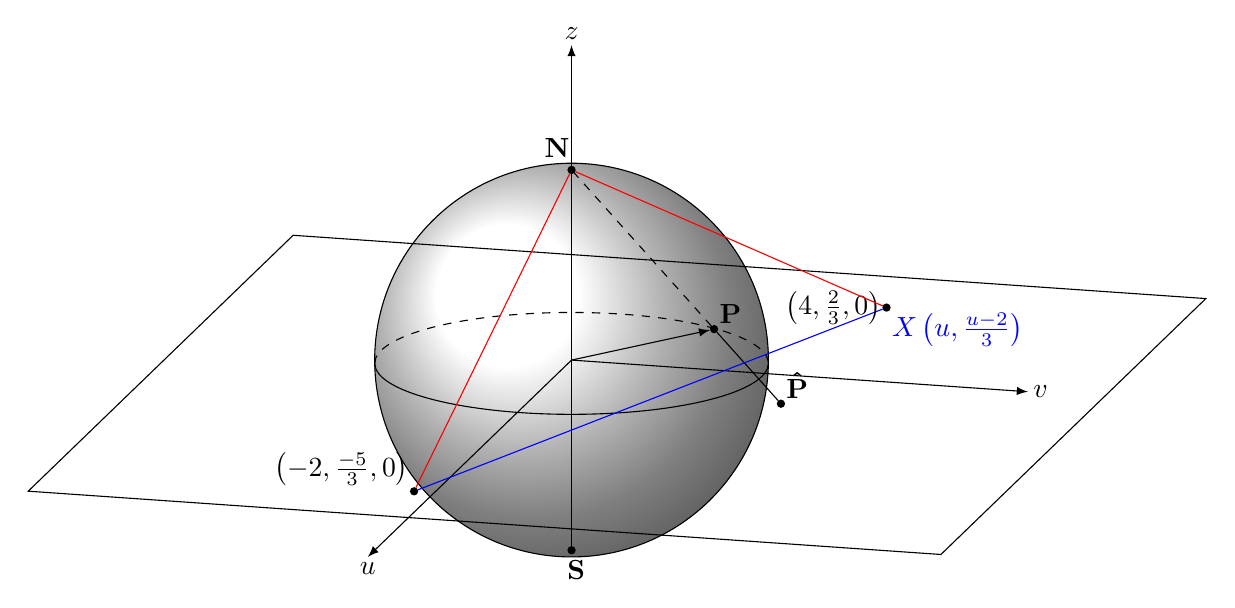
\begin{tikzpicture} % "THE GLOBE" showcase
%Definición de constantes:
\def\R{2.5} % sphere radius
\def\angEl{15} % elevation angle
\def\angAz{-105} % azimuth angle
\def\angPhi{-40} % longitude of point P
\def\angBeta{19} % latitude of point P


%Ecuador
\DrawLatitudeCircle[\R]{0}

\pgfmathsetmacro\H{\R*cos(\angEl)} % distance to north pole

\tikzset{xyplane/.estyle={cm={cos(\angAz),sin(\angAz)*sin(\angEl),-sin(\angAz),
                              cos(\angAz)*sin(\angEl),(0,0)}}}


\LongitudePlane[xzplane]{\angEl}{\angAz}
\LongitudePlane[pzplane]{\angEl}{\angPhi}
\LatitudePlane[equator]{\angEl}{0}

%% draw xyplane and sphere

\fill[ball color=white] (0,0) circle (\R); % 3D lighting effect
\draw(0,0) circle (\R);
\draw[xyplane] (-2*\R,-2*\R) rectangle (3.2*\R,2.8*\R);

\coordinate (O) at (0,0);

\coordinate[mark coordinate] (N) at (0,\H);
\coordinate[mark coordinate] (S) at (0,-\H);

\path[pzplane] (\angBeta:\R) coordinate[mark coordinate] (P);
\path[pzplane] (2.75*\R,\R) coordinate (PE);
\path[xzplane] (0,0) coordinate (XE);
\path (PE) ++ (0,0) coordinate (Paux); % to aid Phat calculation
\coordinate[mark coordinate] (Phat) at (intersection cs: first line={(N)--(P)},
                                        second line={(S)--(Paux)});

\coordinate[mark coordinate] (P1) at (-2,-5/3);

\coordinate[mark coordinate] (P2) at (4,2/3);

\DrawLatitudeCircle[\R]{-1} % equator
\draw[xyplane,<->] (4*\R,0) node[below] {$u$} -- (0,0) -- (0,2.4*\R)
    node[right] {$v$};
\draw[->] (0,-\H) -- (0,1.6*\R) node[above] {$z$};

\draw[dashed] (P) -- (N) +(0.3ex,0.6ex) node[above left] {$\mathbf{N}$};
\draw (P) -- (Phat) node[above right] {$\mathbf{\hat{P}}$};
\path (S) +(0.4ex,-0.4ex) node[below] {$\mathbf{S}$};
\draw[->] (O) -- (P) node[above right] {$\mathbf{P}$};
\draw[blue] (P1) -- (P2) node[below right] {$\mathbb{X}\left(u,\frac{u-2}{3}\right)$};

\path (P1) node [above left] {$\left(-2,\frac{-5}{3},0\right)$};
\path (P2) node [left] {$\left(4,\frac{2}{3},0\right)$};

\draw[red,name=lineP1N] (P1) -- (N);
\draw[red,name=lineP2N] (P2) -- (N);


\end{tikzpicture}



\caption{Proyección estereográfica}
\label{figProyeccionEstereografica}
\end{figure}

Así, todos los puntos del plano están asociados de manera única a un punto de la esfera y viceversa. El único punto sin imagen sería el polo norte al cual le asociamos el infinito.

Por tanto, podemos identificar el plano complejo extendido con una esfera (\textbf{la esfera de Riemann}) mediante la proyección estereográfica:
\[\appl{\psi}{\widehat{\cplex}}{S}\]

\begin{example}
Veamos algunos ejemplos de cómo se comporta esta proyección, a fin de entenderla mejor:
\begin{align*}
\psi\left(\set{z \in \cplex : |z|<1}\right) &= \set{(x_1,x_2,x_3) \in S: x_3<0} \\
\psi\left(\set{z \in \cplex : |z|=1}\right) &= \set{(x_1,x_2,0)\in S} \\
\psi\left(\set{z \in \cplex : |z|>1}\right) &= \set{(x_1,x_2,x_3) \in S: x_3>0}
\end{align*}
\end{example}

Vamos a calcular explícitamente esta aplicación $\psi$.

Sea $z=x+iy$, y lo identificamos con $(x,y,0)$. La recta que pasa por este punto y el polo norte será
\[\{((1-t)x, (1-t)y, t) \tq t \in \real\}\]
y su intersección con la esfera corresponde al $t$ tal que
\[(1-t)^2x^2+(1-t)^2y^2+t^2=1 \iff (1-t)^2|z|^2=1-t^2 \iff (1-t)|z|^{\textcolor{red}{2}}=1+t\]
Despejando llegamos a
\[t = \frac{|z|^2-1}{|z|^2+1}\]

Por tanto, la proyección estereográfica se define como:
\[\psi(z)=\left(\frac{2x}{1+|z|^2},\frac{2y}{1+|z|^2},\frac{|z|^2-1}{|z|^2+1}\right)\]

\obs Para $(x_1,x_2,x_3)\in S\setminus \{(0,0,0)\}$ tenemos que
\[\psi^{-1}((x_1,x_2,x_3))=\frac{x_1+ix_2}{1-x_3}\]

Por último definimos la distancia $\widehat{\dst}$ en $\widehat{\cplex}$ como la distancia entre las imágenes de esos puntos por $\psi$ en $\real^3$. Es decir:
\[\widehat{\dst}(z,w)=||\psi(w)-\psi(z)||\]

\begin{example}
Sean dos complejos $z,w$ vamos a calcular su distancia.

\[\widehat{\dst}(z,w)=||\psi(w)-\Psi(z)||\]
\[(\widehat{\dst}(z,w))^2 = \left( \frac{z+\bar{z}}{1+|z|^2}-\frac{w+\bar{w}}{1+|w|^2}\right)^2-\left( \frac{z-\bar{z}}{1+|z|^2}-\frac{w-\bar{w}}{1+|w|^2}\right)^2 + \left( \frac{|z|^2-1}{1+|z|^2}-\frac{|w|² -1}{1+|w|^2}\right)^2\]

de donde podemos deducir
\[\widehat{\dst}(z,w)=\frac{2|z-w|}{\sqrt{(1+|z|^2)(1+|w|^2)}}\]
\end{example}

Una vez que tenemos definida una distancia podemos hablar de límites y continuidad.

\section{Funciones complejas: límites y continuidad}
En $\cplex$ definimos $\dst(z,w)=|z-w|$

\begin{defn}[Convergencia]
Dada una sucesión $\{z_n\}\in \cplex$
\[\lim_{n \to \infty} z_n = z \iff \forall ε \ \exists N>0 \tq |z_n-z| < ε \ \forall n > N\]

Basándonos en la desigualdad triangular podemos ver que $z_n=a_n+b_ni$ converge a $z=a+bi$ si y sólo si $a_n$ converge a $a$ y $b_n$ converge a $b$.
\end{defn}

En definitiva esta convergencia es equivalente a la convergencia que conocemos en $\real^2$. Por tanto, no nos resultará extraña la siguiente proposición:
\begin{prop}
$(\cplex, d)$ y $(\widehat{\cplex}, \widehat{d})$ son espacios completos.
\end{prop}

\begin{defn}[Continuidad]
Sea $\Omega$ un dominio (abierto y conexo) en $\cplex$ y sea $\appl{f}{\Omega}{\cplex}$ decimos que:
\[\lim_{n\to z_0}f(z)=a \iff \forall ε > 0 \ \exists δ>0 \tq \text{ si } 0 < |z-z_0| < δ \implies |f(z)-a| < ε\]

Decimos que una función $f$ es \textbf{continua} en $z_0$ si $f(z_0) = \lim_{z\to z_0} f(z) = a$
\end{defn}

En el espacio complejo conservamos las propiedades de suma, producto y cociente de límites. La prueba de estas propiedades sería idéntica a la realizada trabajando en $\real^2$ y se deja como ejercicio para el lector desconfiado.

De la misma forma, la suma, producto, cociente y composición de funciones continuas es continua. Esto puede demostrarse de manera trivial una vez probadas las propiedades indicadas en el párrafo anterior.

\begin{problem}[1]
Sean $z_0, w_0 \in \cplex$, demostrar:
\ppart $\displaystyle\lim_{z\to z_0} f(z) = \infty \iff \lim_{z\to z_0}\frac{1}{f(z)}=0$.
\ppart $\displaystyle\lim_{z\to \infty} f(z) = w_0 \iff \lim_{z\to 0}\frac{1}{f(\frac{1}{z})}=\frac{1}{w_0}$.
\ppart $\displaystyle\lim_{z\to \infty} f(z) = \infty \iff \lim_{z\to 0}\frac{1}{f(1/z)}=0$.

\solution
\doneby{Pedro}

En definitiva, todos los apartados se resuelven aplicando las propiedades para el cociente de límites.

\spart
Puesto que
\[\lim_{z\to z_0}\frac{1}{f(z)}=\frac{\lim_{z\to z_0}1}{\lim_{z\to z_0}f(z)}=\frac{1}{\lim_{z\to z_0}f(z)}=0\]
tenemos que la única posibilidad es que $\displaystyle\lim_{z\to z_0}f(z)=\infty$

\spart
\[\lim_{z\to 0}\frac{1}{f(\frac{1}{z})}=\frac{\lim_{z\to 0}1}{\lim_{z\to 0}f(\frac{1}{z})}=\frac{1}{f(\lim_{z\to 0}\frac{1}{z})}=\frac{1}{f(\lim_{z\to \infty}z)}=\frac{1}{\lim_{z\to \infty}f(z)}=w_0\]
Despejando llegamos a
%TODO comprobar que el enunciado sea correcto
\[\lim_{z\to \infty}f(z)=\frac{1}{w_0}\]

\spart
\[\lim_{z\to 0}\frac{1}{f(1/z)}=\frac{\lim_{z\to 0}1}{\lim_{z\to 0}f(1/z)}=\frac{1}{f(\lim_{z\to 0}1/z)} = \frac{1}{f(\lim_{z\to \infty}z)} = \frac{1}{\lim_{z\to \infty}f(z)}=0\]
Una vez más, la única posibilidad es
\[\lim_{z\to \infty} f(x) = \infty\]
\end{problem}


\chapter{Funciones holomorfas}
\begin{defn}[Función\IS holomorfa\IS]
Sea $\Omega \subset \cplex$ abierto y $\appl{f}{\Omega}{\cplex}$ $f$ es \textbf{holomorfa} en $z_0 \in \Omega$ si y sólo si existe
\[\lim_{z\to z_0} \frac{f(z)-f(z_0)}{z-z_0}= f'(z_0)\]

Una función será \textbf{holomorfa} si lo es en todos sus puntos.
\end{defn}

\begin{defn}[Función\IS entera\IS]
Una función es \textbf{entera} si es holomorfa en todo $\cplex$
\end{defn}

\begin{prop}
Si una función $f$ es holomorfa en $z_0$ entonces será continua en ese mismo punto
\end{prop}
\begin{proof}
Basta con considerar
\[f(z)=\frac{f(z)-f(z_0)}{z-z_0}(z-z_0)+f(z_0)\]
sabemos que, por ser $f$ holomorfa,
\[\lim_{z \to z_0}\frac{f(z)-f(z_0)}{z-z_0} = f'(z_0)\]
por lo que
\[\lim_{z \to z_0} f(z) = f'(z_0)\cdot0+f(z_0)=f(z_0)\]
\end{proof}

\section{Derivada compleja}
\begin{itemize}
\item Si $f,g$ son holomorfas en $z_0$ entonces su suma, producto y cociente\footnote{Siempre que el denominador sea no nulo} son holomorfas. Además se conservan las reglas de derivación para estas operaciones.

\item Si $g$ es holomorfa en $z_0$ y $f$ es holomorfa en $g(z_0) \implies$ $f(g(z))$ es holomorfa en $z_0$ y se conserva la regla de la cadena para derivar la composición de funciones.

\item Los polinomios son funciones enteras y podemos calcular su derivada con normalidad.

\item Veremos que si $\exists f'(z_0) \implies \exists f^{(n)}(z_0)\; \forall n \in \nat$, es decir, si una función es derivable una vez entonces lo es infinitas veces.
\end{itemize}

Con la última propiedad hemos obtenido algo realmente nuevo, que no se cumple en las funciones de variable real. A continuación veremos qué le estamos pidiendo a las funciones holomorfas que nos garantiza esto y que no lo pedimos a las funciones de variable real.


\section{Ecuaciones de Cauchy-Riemann}
Sea $\appl{f}{\Omega}{\cplex}$ holomorfa en $z_0=x_0+iy_0$ y sean
\begin{align*}
u(x,y) &= \mop{Re}(f(x+iy)) \\
v(x,y) &= \mop{Im}(f(x+iy))
\end{align*}, entonces podemos escribir $f(x,y)=u(x,y)+iv(x,y)$. Básicamente, hemos definido las funciones $u,v$ que nos dan la parte real e imaginaria respectivamente de la función $f$.

Tenemos que
\[f'(z_0)=\lim_{h \to 0} \frac{f(z_0+h)-f(z_0)}{h}\]
si el límite existe, en cualquier dirección en que me acerque a $z_0$ debo obtener el mismo límite\footnote{Recordad lo que hacíamos en Cálculo II aproximándonos por rectas al trabajar en $\real^2$}.

Esta vez vamos a acercarnos en concreto por dos direcciones, las de los ejes.
\begin{itemize}
\item \textbf{Eje x}
\[f'(z_0)=\lim_{h \to 0} \frac{u(x_0+h,y_0)+iv(x_0+h,y_0)-u(x_0, y_0)-iv(x_0,y_0)}{h}=\]
\[= \lim_{h \to 0}\frac{u(x_0+h,y_0)-u(x_0, y_0)}{h}+i\frac{v(x_0+h,y_0)-v(x_0,y_0)}{h}=\od{u}{x}(x_0,y_0)+i\od{u}{x}(x_0,y_0)\]

En la última igualdad sabemos que las derivadas parciales existen, puesto que el límite de una función compleja puede calcularse como límites de parte real y parte imaginaria.

\item \textbf{Eje y}
\[f'(z_0)=\lim_{k \to 0} \frac{u(x_0,y_0+k)+iv(x_0,y_0+k)-u(x_0, y_0)-iv(x_0,y_0)}{ik}=\]
\[=\frac{1}{i}\left(\od{u}{y}(x_0,y_0)+i \od{v}{y}(x_0, y_0)\right)=\frac{1}{i}\od{f}{y}\]
\end{itemize}

Como ya indicamos, para que la función sea diferenciable, las dos derivadas que acabamos de calcular deberían coincidir. Igualando obtenemos
\[\od{f}{x}(x_0,y_0)= -i \od{f}{y} (x_0,y_0)\]
es decir
\[\od{u}{x}(x_0,y_0)+i\od{v}{x}(x_0,y_0)=-i\left(\od{u}{y}(x_0,y_0)+i\od{v}{y}(x_0,y_0)\right)=\od{v}{y}(x_0,y_0)-i\od{u}{y}(x_0,y_0)\]


Igualando obtenemos las ecuaciones de \textbf{Cauchy-Riemann}.

Por tanto si existe $f'$ existen las 4 derivadas parciales con las que hemos estado trabajando y verifican las ecuaciones de \textbf{Cauchy-Riemann}

\begin{defn}[Ecuaciones\IS de Cauchy-Riemann]
Las \textbf{ecuaciones de Cauchy-Riemann} son dos ecuaciones diferenciales parciales que son básicas en el análisis de funciones complejas de variable compleja, debido a que su verificación constituye una condición necesaria (aunque no suficiente) para la derivabilidad de este tipo de funciones.

Estas ecuaciones son:
\begin{align*}
\dpa{u}{x}(x_0,y_0) &= \dpa{v}{y}(x_0,y_0) \\
\dpa{v}{x}(x_0,y_0) &= -\dpa{u}{y}(x_0,y_0)
\end{align*}
\end{defn}

\section{Funciones armónicas}

Si $u,v\in \cplex^2(\Omega)$ y satisfacen las ecuaciones de Cauchy-Riemann (C-R), entonces, derivando a ambos lados de las ecuaciones C-R, obtenemos:
\[\od[2]{u}{x}= \frac{\dif^2 v}{\dif x \dif y}, \ \ \od[2]{v}{y}= \frac{\dif u^2}{\dif y \dif x} \]
\[\od[2]{u}{y}=-\frac{\dif^2 v}{\dif y \dif x}, \ \ \od[2]{v}{x}=-\frac{\dif u^2}{\dif x \dif y} \]

Por tanto, puesto que el orden de derivación no influye, tenemos que
\[\od[2]{u}{x}+\od[2]{u}{y} = 0 \quad \od[2]{v}{x}+\od[2]{v}{y} = 0\]

\newpage
\begin{defn}[Laplaciano]
El laplaciano u operador de Laplace se aplica sobre funciones y consiste en sumar las segundas derivadas respecto de cada variable. Es decir:
\[ Δ(f(x,y)) = \od[2]{f}{x}+\od[2]{f}{y}\]
siendo $f(x,y)=\underbrace{\mop{Re}(x,y)}_{u(x,y)}+\underbrace{\mop{Im}(x,y)}_{v(x,y)}i$
\end{defn}

\begin{defn}[Función\IS armónica]
Se dice que una función es \textbf{armónica} si su laplaciano es 0.
\end{defn}

\begin{prop}
Si $u,v \in \cplex^2(\Omega)$ y verifican las ecuaciones de Cauchy-Riemann entonces su parte real y su parte imaginaria son armónicas.
\end{prop}

Como veremos que la derivada de una función holomorfa es holomorfa, entonces $u,v$ tendrán derivadas parciales de todos los órdenes.

Por tanto, si $f=u+iv$ es holomorfa en $\Omega$ entonces $u,v$ son \textbf{armónicas} en $\Omega$

%\obs Si $\Omega$ es simplemente conexo y $u$ es arḿónica en $\Omega$, entonces existirá una función $f$ holomorfa en $\Omega$ tal que $f=u+iv$

\begin{prop}
Supongamos que tenemos dos funciones $u,v$ diferenciables en $(x_0,y_0)$ (por ejemplo, existen las derivadas parciales en ese punto y son continuas en un entorno del mismo)\footnote{Recordamos que si era diferenciable teníamos esta propiedad pero no al revés.} y que verifican las ecuaciones de Cauchy-Riemann, entonces $f=u+iv$ es holomorfa en $z_0=x_0+iy_0$
\end{prop}
\begin{proof}
Tenemos las dos funciones $\appl{u,v}{\real^2}{\real}$ diferenciables. Por ser diferenciables en $(x_0,y_0)$ sabemos que
\begin{gather*}
u(x_0+α,y_0+β)-u(x_0,y_0)=\od{u}{x}(x_0,y_0)α+\od{u}{y}(x_0,y_0)β + o\left(||(α,β)||\right) \\
v(x_0+α,y_0+β)-v(x_0,y_0)=\od{v}{x}(x_0,y_0)α+\od{v}{y}(x_0,y_0)β + o\left(||(α,β)||\right)
\end{gather*} usando el desarrollo de Taylor.

Para que $f$ fuese holomorfa necesitamos que exista la derivada. Vamos a verlo:

\begin{align*}
\overbrace{f(x_0+iv_0+α+βi)}^{f(z_0+μ)}-\overbrace{f(x_0+iy_0)}^{f(z_0)}  &= u(x_0+α,y_0+β)-u(x_0,y_0) + \\
&\qquad + i \left( v(x_0+α,y_0+β)-v(x_0,y_0)\right) = \\
&= \od{u}{x}(x_0,y_0)α+\od{u}{y}(x_0,y_0)β + o(||(α,β)||) + \\
&\qquad + i\left( \od{v}{x}(x_0,y_0)α+\od{v}{y}(x_0,y_0)β + o(||(α,β)||)\right)
\end{align*}

Pero, puesto que tanto $u$ como $v$ verifican las ecuaciones de Cauchy-Riemann, podemos escribir:
\[\od{u}{y}(x_0,y_0)=-\od{v}{x}(x_0,y_0), \quad \od{v}{y}(x_0,y_0)=\od{u}{x}(x_0,y_0) \]
y aplicando estos cambios en la igualdad anterior tendríamos:
\[\od{u}{x}(x_0,y_0)α-\od{v}{x}(x_0,y_0)β + o(||(α,β)||)+i\left( \od{v}{x}(x_0,y_0)α+\od{u}{x}(x_0,y_0)β + o(||(α,β)||)\right)=\]
\[=\left(\od{u}{x}(x_0,y_0)+i\od{v}{x}(x_0,y_0)\right)(α+iβ)+o(|α+iβ|)\]
Para garantizar que $f$ es holomorfa deberíamos ver que:
\[\lim_{h\to 0} \frac{f(z_0+h)-f(z_0)}{h} = \lim_{α,β->0} \frac{\left(\od{u}{x}(x_0,y_0)+i\od{v}{x}(x_0,y_0)\right)(α+iβ)+o(|α+iβ|)}{α+βi} = \]
\[= \left(\od{u}{x}(x_0,y_0)+i\od{v}{x}(x_0,y_0)\right)\]

Así, queda claro que la derivada de $f$ existe por lo que $f$ es holomorfa.
\end{proof}

Veamos ahora algo de notación.

\begin{defn}[Notación:\IS$\partial$]
Sea una función $\appl{f}{\cplex}{\cplex}$ definimos
\[\partial f = \partial_z f = \frac{1}{2}(d_x f - i d_y f)\]
\end{defn}

\begin{defn}[Notación:\IS$\bar{\partial}$]
Sea una función $\appl{f}{\cplex}{\cplex}$ definimos
\[\bar{\partial} f = \partial_{\bar{z}} f = \frac{1}{2}(d_x f + i d_y f)\]
\end{defn}

Formalmente, si consideramos a $f$ como una función de $z$ y $\bar{z}$ tenemos que
\[x = \frac{z+\bar{z}}{2}, \ \ y = \frac{z-\bar{z}}{2i}\]
de donde, derivando, obtenemos que
\[\od{x}{z}=\frac{1}{2}, \ \od{x}{\bar{z}}=\frac{1}{2}, \ \od{y}{z}=\frac{1}{2i}, \ \od{y}{\bar{z}}=\frac{1}{2i},\]
Ahora podemos aplicar la regla de la cadena y calcular
\[\partial_z f = \partial_x f \frac{1}{2}+\partial_u f \frac{1}{2i}\]
\[\partial_{\bar{z}} f = \partial_x f \frac{1}{2}+\partial_u f \left(-\frac{1}{2i}\right)\]

\begin{prop} $f$ es holomorfa si y sólo si $\bar{\partial}f=0$.
\end{prop}
\begin{proof}
Si la función $f$ es holomorfa, sabemos que verifica las ecuaciones de Cauchy-Riemann. Así
\[\bar{\partial}_z f = \frac{1}{z}(\dif_x f + i \dif_y f) = \frac{1}{z} \left(\od{f}{x}+i\od{f}{y} \right) = \frac{1}{z} \left( \od{u}{x}+i\od{v}{x} + i \od{u}{y} - \od{v}{y}\right) \eqexpl{C-R} \]
\[=\frac{1}{z} \left( \od{v}{y}-i\od{u}{y} + i \od{u}{y} - \od{v}{y}\right) = 0\]
\end{proof}

\begin{prop}
\[f(z)-f(z_0)=\partial_xf(z_0)\left(\frac{z+\bar{z}-z_0-\bar{z}_0}{2}\right)-i\partial_y f (z_0)\left( \frac{z-\bar{z}-z_0+\bar{z}_0}{2}\right) + o (|z-z_0|)\]
y aplicando las definiciones (notación) dadas anteriormente, tenemos
\[f(z)-f(z_0)= \partial f(z_0)(z-\bar{z}_0)+\bar{\partial}f(z_0)(\bar{z}-\bar{z}_0)+o|z-z_0|\]

Es decir, podemos escribir $f$ en función de $z$ y su derivada en función de las definiciones $\partial$ y $\bar{\partial}$.
\end{prop}

\begin{example}
\begin{enumerate}
\item
\[f(z)=\frac{z^2}{(z^2+1)^2}\]
Esta función es holomorfa en $\cplex\setminus\{\pm i\}$. Para verlo nos basamos en que es el cociente de dos funciones holomorfas por lo que $f(z)$ será holomorfa en todo $\cplex$ salvo los puntos en que se anula el denominador.

Si calculamos la derivada obtenemos
\[f'(z)=\frac{2z(z^2+1)^2-z^22(z^2+1)2z}{(z^2+1)^4}\]
y vemos que, efectivamente, existe para todo $z \in \cplex\setminus\{\pm i\}$

\item
\[f(z)=z\cdot \mop{Re}(z)\]
Vamos a reescribir esta función de la forma:
\[f(z)=(x+iy)x = x^2 + ixy\]
Si escribimos $f(x,y)=u(x,y) + i v(x,y)$ tenemos que $ u(x,y)=x^2$ y $v(x,y)=xy$. Vamos a ver si satisfacen las ecuaciones de Cauchy-Riemann.

\begin{align*}
\partial_x f &= -i \partial_yf \\
u_x+iv_x &= -i (u_y+iv_y) \\
\end{align*}

Para que se cumplan las ecuaciones de Cauchy-Riemann necesitamos que $u_x=v_y$ y que $u_y=-v_x$, ecuaciones que se satisfacen únicamente en $(0,0)$, punto en el que son diferenciables tanto $u$ como $v$.

\obs Podríamos haber comprobado que la función no es holomorfa mediante la definición o escribiendo:
\[f(z)=z\left( \frac{z+\bar{z}}{2}\right)=\frac{z^2}{2}+\frac{z}{2}\bar{z}\]
Tenemos pues que $\bar{\partial}f=\frac{z}{2}$ que sólo se anulará en $z=0$.

\item
\[f(z) = \left\{ \begin{array}{lcc}
   \frac{z^5}{|z|^4} & si & z \neq 0 \\
   \\ 0 & si & x = 0 \end{array} \right.\]

En primer lugar vemos que la función es continua en $z=0$ pues
\[\lim_{z \to 0} \frac{z^5}{|z|^4} = 0 = f(0)\]

Sabemos que el límite es 0 pues aplicando la definición directamente obtenemos que
\[\forall ε > 0 \exists δ > 0 \tq \text{ si } 0<|z|<δ \implies \left|\frac{z^5}{|z|^4}\right| = |z| < ε\].

Veamos ahora si es una función holomorfa. Para ello tenemos que calcular el límite
\[\lim_{z \to 0} \frac{f(z)}{z}\]
En este caso, vamos a ver que no existe y para ello vamos a acercarnos por dos rectas diferentes: el eje real y la recta $z=|z|e^{iα}=re^{iα}$.

Obtenemos los siguientes resultados
\[\lim_{x \to 0} \frac{x^5}{|x|^4x} = \lim_{x \to 0} 1 = 1\]
\[\lim_{r \to 0} \frac{r^4 e^{i4α}}{r^4} = e^{i4α} \neq 1\]

Por tanto, el límite no existe y la función \textbf{no es holomorfa}. Sin embargo, las ecuaciones de Cauchy-Riemann si se satisfacen para esta función, con lo que queda claro que \textbf{las ecuaciones de Cauchy-Riemann no son condición suficiente para que la función sea holomorfa}.
\end{enumerate}
\end{example}

\section{Teorema de la función inversa}
\begin{theorem}[Teorema\IS de la función inversa]
Sea $\appl{f}{\Omega\subset \cplex}{\cplex}$ holomorfa siendo $\Omega$ un abierto con $z_0\in \Omega$.

Existe un entorno $U_{z_0}\subset \Omega$ de $z_0$ tal que $f|_{U_{z_0}}$ es un isomorfismo holomorfo (biyectiva, holomorfa y con inversa holomorfa) si y sólo si $f'(z_0)=0$
\end{theorem}
\begin{proof}
Vamos a demostrarlo apoyándonos en el ya conocido teorema de la función inversa para $\real^2$.

Sea $f(x,y)=u(x,y)+iv(x,y)$ definimos la función
\[\appl{g}{\real^2}{\real^2}\]
que nos lleva el punto $(x,y)$ a $\left( u(x,y), v(x,y)\right)$

Esta función tendrá inversa en el punto $(x_0,y_0)$ si su Jacobiano es distinto de 0 en ese punto. Vamos a calcularlo
\[ J_g(x_0,y_0) = \left| \begin{array}{cc}
u_x(x_0,y_0) & u_y(x_0,y_0)\\
v_x(x_0,y_0) & v_y(x_0,y_0) \end{array} \right| = u_x(x_0,y_0)v_y(x_0,y_0)-u_y(x_0,y_0)v_x(x_0,y_0) \eqexpl{C-R}\]
\[\eqexpl{C-R} \left(u_x(x_0,y_0)\right)^2 +\left(v_x(x_0,y_0)\right)^2 = \left(u_y(x_0,y_0)\right)^2 +\left(v_y(x_0,y_0)\right)^2 = |f'(z_0)|^2\]

Puesto que $f$ es un isomorfismo holomorfo, sabemos que es un isomorfismo diferenciable pues veremos un resultado que garantiza que siendo $f$ holomorfa, sabemos que $f'$ también lo es y por tanto $u,v \in \cplex^{\infty}$.

Por tanto ya tenemos que, siendo $f$ una función holomorfa que tiene función inversa, es necesario que $f'(z_0)\neq 0$.

Para probar la implicación contraria, si $f'(z_0) \neq 0$ tenemos, por el teorema de la función inversa en los reales, que existe $g^{-1}(h,k)$, la función inversa de $g$ en un entorno de $(x_0,y_0)$. Simplemente nos quedaría ver que $h+ik$ es holomorfa.

Sea $f(z)=α+βi$ la matriz Jacobiana en $(α,β)$ es
\[\left( \begin{array}{cc}
h_x(x_0,y_0) & h_y(x_0,y_0)\\
k_x(x_0,y_0) & k_y(x_0,y_0) \end{array} \right) = \left( \begin{array}{cc}
u_x(x_0,y_0) & u_y(x_0,y_0)\\
v_x(x_0,y_0) & v_y(x_0,y_0) \end{array} \right)^{-1}=\]
\[=\frac{1}{|f'(z)|^2}\left| \begin{array}{cc}
v_y(x_0,y_0) & -u_y(x_0,y_0)\\
-v_x(x_0,y_0) & v_x(x_0,y_0) \end{array} \right| \eqexpl{C-R} \frac{1}{|f'(z)|^2}\left| \begin{array}{cc}
u_x(x_0,y_0) & -u_y(x_0,y_0)\\
-u_x(x_0,y_0) & u_y(x_0,y_0) \end{array} \right| \]
De ahí podemos extraer que $h(α,β)$ y $k(α,β)$ verifican las ecuaciones de Cauchy-Riemann.

Además,
\[g^{-1}(f(z))=h_x(f(z))+ik_x(f(z)) = \frac{1}{|f'(z)|^2}\left( u_x(x,y)-iv_x(x,y)\right) = \frac{f'(z)}{|f'(z)|^2} = \frac{1}{f'(z)}\]

\end{proof}

\section{Series de potencias}
Sea $\{z_n=x_n+iy_n\}$ una sucesión en $\cplex$,
\[\lim_{n \to \infty}z_n=z \iff \forall ε > 0 \ \exists N \tq |z_n-z| \leq ε \ \forall n \geq N\]

Además, como
\[|x_n-x|<|z_n-z|<|x_n-x|+|y_n-y|\]
la sucesión $z_n$ convergerá sii lo hacen las sucesiones $x_n$ e $y_n$.

Siempre que exista ese número complejo, $z$, diremos que la sucesión \concept{converge}. Si no existe este límite, diremos que la sucesión \concept{diverge}. En particular, si $\lim_{n \to \infty}|z_n|=\infty$ diremos que \concept{diverge a $\infty$}.

Esta divergencia a infinito tiene sentido cuando trabajamos con el plano complejo extendido (recordemos que era el plano complejo al que habíamos añadido el infinito). Para que la \textbf{divergencia a infinito} tenga auténtico sentido debemos observar la sucesión en la esfera de Riemann donde veríamos que esta ``va hacia el polo norte''

\begin{defn}[Serie]
En matemáticas, una \textbf{serie} es la generalización de la noción de suma a los términos de una sucesión infinita. Informalmente, es el resultado de sumar los términos: $a_1 + a_2 +a_3 + a_4 + a_5 + a_6 \dots $ lo cual suele escribirse en forma más compacta como $\sum_{1\le n} a_n$.

El estudio de las series consiste en la evaluación de la suma de un número finito n de términos sucesivos y, mediante un pasaje al límite, identificar el comportamiento de la serie a medida que n crece indefinidamente.
\end{defn}

Una serie $\sum z_n$ converge a $w$ si y sólo si $\lim_{n \to \infty}\sum_{k=1}^n z_k = w$. En este caso escribimos
\[\sum_{k=1}^{\infty}z_k = w\]

Veamos algunas propiedades acerca de las series
\begin{itemize}
\item Si $\sum z_n$ converge, entonces
\[\lim_{n \to \infty} z_n = 0\]

Esto es sencillo de entender puesto que si una suma infinita converge a un número necesitamos que los sumandos converjan a 0. De lo contrario siempre estaríamos sumando algo no despreciable y la suma infinita tendería a infinito.

\item Sea $s_n=\sum_{k=1}^{n} z_n$,

\begin{defn}[Sucesión\IS de Cauchy]
\[\{s_n\} \text{ es de Cauchy} \iff \forall δ > \ \exists N \tq \text{ si } n,m \geq N \implies |s_n-s_m| < ε\]
\end{defn}

\item Si $\sum | z_n| $ converge entonces $\sum z_n$ también converge.

\begin{proof}
Sean $s_n = \sum_{k=1}^n z_k$ y $s_n'=\sum_{k=1}^n |z_k|$ vamos a probar que $s_n$ converge. Para ver que converge vamos a probar que es de Cauchy.

\[|s_m - s_n| = \left|\sum_{k=m+1}^m z_k\right| \leq \sum_{k=n+1} ^m | z_k| = |s_m'-s_n'| < ε\]

Puesto que sabemos que $s_n'$ es de Cauchy queda claro que la sucesión $s_n$ también lo es, pues la distancia entre dos elementos de esta segunda sucesión es siempre menor que la diferencia entre dos elementos de la primera sucesión, que es de Cauchy.

\end{proof}

\end{itemize}

\begin{defn}[Convergencia\IS absoluta]
Si la serie $\sum |z_n|$ converge diremos que $\sum z_n$ converge absolutamente.
\end{defn}

\begin{defn}[Convergencia\IS puntual]
Sea $\{\appl{f_n}{\Omega\subset \cplex}{\cplex}\}$ una sucesión de funciones, decimos que $\{f_n\}$ converge puntualmente a $\appl{f}{\Omega\subset\cplex}{\cplex}$ sii converge punto a punto. Es decir
\[f_n(z) \rightarrow f(z) \iff \lim_{n\to\infty}f_n(z)=f(z) \forall z \in \Omega \iff\]
\[\iff \forall ε > 0 \forall z \in \Omega \exists N=N(ε,z) \tq \forall n \geq N |f_n(z)-f(z)| < ε \]
\end{defn}

\begin{defn}[Convergencia\IS uniforme]
Sea $\{\appl{f_n}{\Omega\subset \cplex}{\cplex}\}$ una sucesión de funciones, decimos que $\{f_n\}$ converge uniformemente a $\appl{f}{\Omega\subset\cplex}{\cplex}$ si ``tenemos convergencia puntual con un único $N(z)$ para todo $z$''. Es decir
\[f_n \rightrightarrows f \iff \forall ε >0 \ \exists N=N(ε) \tq \forall n \geq N \ |f_n(z)-f(z)| < ε \; \forall z \in \Omega\]
\end{defn}

\begin{prop}[Criterio\IS M de Weierstrass]
Sea $\appl{f_n}{\Omega}{\cplex}$ funciones tales que $|f_n(z)| \leq M_n$ para todo $z \in \Omega$ con $M_n$ una sucesión de números positivos. Si $\sum M_n$ converge, entonces $\sum f_n$ converge \textbf{absoluta} y \textbf{uniformemente}.
\end{prop}

\begin{proof}
Primero debemos determinar quién es ese límite antes de poder llevar a cabo la demostración.

Sea $g_n(z)=\sum_{k=1}^{n}f_k(z)$ podemos ver que es una sucesión de Cauchy, pues
\[|g_m(z)-g_n(z) | = \left|\sum_{k=n+1}^m f_k(z)\right| \leq \sum_{k=n+1}^m | f_k(z)| \leq \sum_{k=n+1}^m M_k = |s_m-s_n|\footnote{siendo $s_n = \sum_{i=1}^n M_i$} < ε\]

La última desigualdad la obtenemos del hecho de que $M_n$ es convergente y por tanto es de Cauchy.

Por tanto, tenemos que la sucesión $g_n$ también es de Cauchy por lo que converge. Así, podemos definir límite como $g(z)=\lim_{n\to \infty}g_n(z)$ pero, si nos fijamos, tenemos que
\[g(z)=\lim_{n\to \infty}g_n(z) = \lim_{n\to \infty}\sum_{k=1}^n f_k(z) = \sum_{k=1}^{\infty} f_k(z)\]
por lo que, efectivamente, hemos probado que la suma de las $f_n$ converge.

Ahora nos queda probar que la convergencia es uniforme pues, con los pasos realizados hasta ahora, sólo podemos garantizar la convergencia puntual.

Vamos a ello
\[|g_n(z)-g(z)| = \lim_{k \to \infty}|g_n(z)-g_{n+k}(z)|\]
Dado ε > 0 $\exists N$ t.q.  $\forall n \geq N$, $|g_n(z)-g_{n+k}(z)| < ε \ \forall z \in \Omega$.

Así, queda probada la convergencia uniforme.
%TODO completar por que el final de la demostración no dice nada
\end{proof}

\begin{defn}[Serie\IS centrada]
Una series de potencias \textbf{centrada en $z_0 \in \cplex$} es una serie de la forma
\[\sum_{n=0}^{\infty} a_n(z-z_0)^n\]
\end{defn}

\begin{example}
Dada la serie geométrica $\sum_{n=0}^{\infty}z_n^n$ podemos ver que
\[(1-z)(1+z+z^2+...z^n)=1-z^{n+1}\]
para $z \neq 1$ de donde podemos deducir que
\[1+z+z^2+...+z^n = \frac{1-z^{n+1}}{1-z}\]
(en los ejercicios podemos encontrar una demostración por inducción de esta fórmula)

Vamos a analizar ahora el resultado obtenido viendo el límite de estas series.
\begin{itemize}
\item \textbf{Si |z| < 1}
\[\lim_{n \to \infty} z^n = 0\]
\[\sum z^n =\lim_{n \to \infty}\sum_{i=0}^{\infty} \frac{1}{1-z}\]
\item \textbf{Si |z| > 1}
\[\lim_{n \to \infty} z^n = \infty\]
La serie diverge, luego su suma será infinita.
\end{itemize}
\end{example}

\begin{prop}
Consideremos la serie de potencias
\[\sum_{n=0}^{\infty} a_n (z-z_0)^n\]
y supongamos que $\exists ε \in \cplex$ tal que
\[|a_n||ε|^n \leq M \ \forall n\]
con $M$ constante.

Entonces, para todo $\rho ∈ (0, |ε|)$ la serie converge absoluta y uniformemente en $\{z \tq |z-z_0| < \rho\}$.
\end{prop}
\begin{proof}
Si $|z-z_0 | \leq \rho < |ε|$ tenemos que
\[|a_n(z-z_n)^n| = |a_n||z-z_0|^n=|a_n||ε|^n\frac{|z-z_0|^n}{|ε|^n}\leq M \left( \frac{\rho}{|ε|}\right)^n\]
Como $\sum \left( \frac{\rho}{|ε|}\right)$ converge obtenemos el resultado buscado por el criterio M de Weierstrass.
\end{proof}

Básicamente ese ε nos va a dar el tamaño de la bola centrada en $z_0$ que nos permite garantizar la convergencia y, obviamente, estamos interesados en localizar el mayor ε. Siendo $α = \abs{z-z_0}$, tenemos dos posibilidades:
\begin{enumerate}
\item $\displaystyle \forall α > 0 \ \sup_n|a_n|α^n < \infty$

En este caso tenemos convergencia en el disco $|z-z_0|<α \ \forall α$. Se trata de un caso \textbf{ideal} en el que la serie converge en todo $\cplex$

\item $\displaystyle \exists α > 0 \tq \sup_n|a_n|α^n = \infty$

En este caso nos gustaría encontrar el mayor α posible sin que el supremo indicado se haga infinito.

\obs $\phi(α)=\sum_n|a_n|α^n$ es una función creciente. Por tanto, dada una sucesión $α_1<α_2,...$ sabemos que si $\phi(α_2) < \infty \implies \phi(α_1) < \infty$ y que si $\phi(α_2)=\infty \implies \phi(α_3) = \infty$.

Por tanto, queremos buscar justo el punto en que esta función pasa de ser finita a ser infinita.
\end{enumerate}

\begin{defn}[Radio\IS de convergencia]
El \textbf{radio de convergencia de la serie} se define como
\[R=\inf \{α > 0\tq \sup_n|a_n|α^n = \infty\}\]
de forma totalmente equivalente podemos definir este radio de la siguiente forma
\[R=\sup \{α > 0\tq \sup_n|a_n|α^n < \infty\}\]
\end{defn}

Evidentemente, por la propia definición del radio de convergencia, la serie converge en el interior de la bola $|z-z_0|<R$ y diverge fuera de la misma.

La frontera ($|z-z_0|=R$) es un caso extremo que habría que analizar detenidamente en cada caso particular.

Hasta ahora hemos dejado claro la importancia de este radio de convergencia y la teoría acerca de cómo calcularlo, pero no es viable calcular un ínfimo sobre todos los posibles complejos que cumplen una cierta condición.

Necesitamos una fórmula para calcular este radio y el siguiente teorema nos la da:

\begin{theorem}
Sea $R$ el radio de convergencia de la serie de potencias $\sum_{n=0}^{\infty} a_n (z-z_0)^n$. Se tiene que \[R = \frac{1}{\limsup_{n \to \infty} |a_n|^{1/n}}\]

Además, si $a_n \neq 0\; \forall n$ y existe el límite \[ \lim_{n \to \infty} \left|\frac{a_n}{a_{n+1}}\right|\] (pudiendo ser infinito), entonces \[ R = \lim_{n \to \infty}\frac{|a_n|}{|a_{n+1}|}\]

La serie converge uniformemente en $\{z \tq |z-z_0| < r\}$ con $r \leq R$ y converge absolutamente en $\{z \tq |z-z_0|<R\}$.
\end{theorem}
\begin{proof}

\begin{enumerate}
\item Lo primero que debemos hacer es comprobar que esta fórmula para $R$ coincide con la definición del mismo dada anteriormente.

Supongamos que $0<R<\infty$ (calculando $R$ según su definición). Vamos a probar la igualdad dividiendo en dos desigualdades. Buscamos probar primero que
\[\limsup_{n \to \infty} |a_n|^{1/n} \leq \frac{1}{R}\]

Dado que $R$ es finito, existe un $r∈(0,R)$ tal que $\sup_n |a_n| r^n <\infty$\footnote{Guille: Yo diría que esto se cumple para todo $r$ en $(0,R)$ por definición, ¿no?}. En este caso existe un $M>0$ tal que $|a_n|r^n < M \ \forall n ∈ ℕ$.

Así, tendríamos que $|a_n|^{1/n} < \frac{M^{1/n}}{r}$ y en el infinito veríamos que
\[\lim_{n \to \infty} |a_n|^{1/n} \leq \frac{1}{r} \ \forall r ∈ (0,R) \implies \limsup_{n \to \infty}|a_n|^{1/n} \leq \frac{1}{R}\]

Si conseguimos probar ahora la desigualdad contraria habremos logrado demostrar la igualdad, es decir, habremos demostrado que la fórmula dada para el cálculo de $R$ encaja con la definición del mismo.

Vamos a probar esta desigualdad por reducción al absurdo: vamos a ver qué ocurre si el límite ese es menor que $\frac{1}{R}$ (que es lo mismo que decir que no sea mayor o igual):
\[\limsup_{n \to \infty}|a_n|^{1/n} < \frac{1}{R} \implies \exists N > 0 \tq \forall n \geq N \ \sup_{k \geq N} |a_n|^{1/n} < \frac{1}{r} < \frac{1}{R} \implies\]
\[\implies \forall k \geq N \ |a_k|^{1/k} < \frac{1}{r} \implies |a_n| r^n < M \forall n \implies \sup_{n\to\infty}|a_n|r^n< \infty\]
pero teníamos que $R > r$ lo que nos lleva a contradicción, pues la R marca el límite a partir del cual la serie deja de ser convergente.
\item
Sea β$= \lim_{n \to \infty}\left|\frac{a_n}{a_{n+1}} \right|$

Si vemos que la serie converge en $\{z: |z-z_0| < r^-\} \ \forall r^-<β$, tendremos que β $\leq R$.

Como $r^- < β$ existe un $N$ t.q. $r^-<\left|\frac{a_n}{a_{n+1}} \right| \forall n \geq N$, es decir:
\[a_{n+1} < \frac{|a_n|}{r^-}\]
desplazándonos un término a la izquierda en la sucesión ($n-1$) y multiplicando a ambos lados por $(r^-)^n$ obtenemos
\[|a_n|(r^-)^n < \frac{|a_{n-1}|(r^-)^n}{r^-} = |a_{n-1}|(r^-)^{n-1}<\frac{|a_{n-2}|(r^-)^{n-1}}{r^-}=|a_{n-2}|(r^-)^{n-2} \leq ... \leq M\]

Así, podemos escribir
\[\sum_n |a_n(z-z_0)^n|=\sum_n |a_n|(r^-)^n\left(\frac{|z-z_0|}{r^-}\right)^n \leq M \sum \left( \frac{|z-z_0|}{r^-}\right)^n\]
que es convergente para $|z-z_0|<r^-$

Por tanto, tenemos que $β \leq R$. Sólo nos queda demostrar la desigualdad contraria para poder concluir la igualdad.

Si vemos que la serie diverge en $|z-z_0|>r^+ \ \forall r^+ > β$, tendremos que $r^+\geq R$. Vamos a ello

Como $r^+ > β$ existe un $N$ t.q. $r^+>\left|\frac{a_n}{a_{n+1}} \right| \forall n \geq N$, es decir:
\[|a_{n+1}| r^+ \geq |a_n|\]
y repitiendo las cuentas del apartado anterior podemos llegar a
\[|a_n|(r^+)^n \geq M\]

Así, podemos escribir
\[\sum_n |a_n(z-z_0)^n|=\sum_n |a_n|(r^+)^n\left(\frac{|z-z_0|}{r^+}\right)^n \geq M \sum \left( \frac{|z-z_0|}{r^+}\right)^n\]
que es divergente para $|z-z_0|>r^+$.

Por tanto, obtenemos claramente que $β \geq R$ por lo que, finalmente, podemos concluir
\[β=R=\lim_{n \to \infty}\frac{|a_n|}{|a_{n+1}|}\]

\item La demostración es idéntica a una realizada anteriormente y se deja como ejercicio para el lector.
\end{enumerate}
\end{proof}


Veamos algunas muestras de la relación de este resultado con nuestros conocimientos sobre los reales. Puesto que los reales son parte de los complejos, deberán cumplirse las condiciones de convergencia sobre ellos
\begin{itemize}
\item
Sea $\sum a_n$ una serie compleja y sea $c=\limsup_{n \to \infty} |a_n|^{1/n}$; si $c<1$ la serie converge y si $c > 1$ diverge.

Esta $c$ aparecía al definir el radio de convergencia como el inverso del mismo por lo que esta resultado puede escribirse como; $R>1$ implica que la serie converge y si $R<1$ diverge.

\item
Recordemos de los reales que si $\exists \lim_{n \to \infty} \frac{a_{n+1}}{|a_n|} = D \implies$ si $D > 1$ la serie diverge y si es menor que 1, converge.

Nuevamente esto puede probarse con el teorema anterior considerando que $D=\frac{1}{R}$. Por tanto, $D>1 \implies R < 1\implies$ divergencia y viceversa.

\end{itemize}

Veamos algunos ejemplos del estudio de convergencia de series
\begin{example}
\begin{enumerate}
\item
Tomemos la serie
\[\sum_{n=1}^{\infty} \frac{(2n)!}{(n)!}z^n\]
en este caso
\[R = \lim_{n \to \infty} \frac{|a_n|}{|a_{n+1}|} = \lim_{n \to \infty} \frac{(2n)!((n+1)!)^2}{(n!)^2(2(n+1))!} = \lim_{n \to \infty} \frac{(n+1)^2}{(2n+2)(2n+1)} = \frac{1}{4}\]

\item
Tomemos la serie
\[\sum_{n=0}^{\infty} z^{n!} = \sum_{k=0}^{\infty}a_k z^k \text{ con } a_k = 1 \iff k=n!\]

En este caso
\[\limsup|a_k|^{1/k} = 1 \implies R = 1\]

\end{enumerate}
\end{example}

Vamos a estudiar ahora cómo se relacionan los radios de convergencia para la suma y el producto mediante un ejemplo.
\begin{example}[Comportamiento de los radios de convergencia frente a la suma y el producto]
Sea $\sum a_nz^n$ con radio de convergencia $R_1$ y $\sum b_n z^n$ con radio de convergencia $R_2$ tenemos:
\begin{enumerate}
\item $\displaystyle \sum_{n=0}^{\infty}(a_n\pm b_n)z^n \implies R = \min\{R_1, R_2\}$
ya que podemos escribir la suma como
\[\sum_{n=0}^{\infty}(a_n\pm b_n)z^n = \lim_{n \to \infty} \sum_{i=0}^n (a_i\pm b_i)z^i\]
y ese límite podrá descomponerse en suma de límites cuando ambos límites existan. La forma de garantizar que esto ocurra es tomar el mínimo de los radios de convergencia.

\item $\displaystyle  \sum_{n=0}^{\infty} a_nb_nz^n$

Podemos operar y ver que
\begin{multline*} \frac{1}{R}=\limsup_{ n \to \infty}|a_nb_n|^{1/n} = \limsup_{n\to \infty}|a_n|^{1/n}|b_n|^{1/n} \leq\\
\leq \limsup_{n\to \infty} |a_n|^{1/n}\cdot \limsup_{n\to \infty} |b_n|^{1/n} = \frac{1}{R_1}\frac{1}{R_2} \end{multline*}

Por tanto tenemos que $R \geq R_1R_2$ y tendremos la igualdad cuando exista al menos uno de los límites superiores: $\limsup_{n\to \infty} |a_n|^{1/n}$ ó $\limsup_{n\to \infty}|b_n|^{1/n}$.

Para afirmar esto nos hemos basado en el siguiente lema:
\begin{lemma}
Sean $x_n,y_n \geq 0$,
\[\exists \lim_{n \to \infty} x_n \implies \limsup_{n \to \infty }(x_ny_n)=\lim_{n \to \infty}x_n \cdot \limsup_{n \to \infty} y_n\]
\end{lemma}

\item $\displaystyle \sum_{n = 0}^{\infty} \frac{a_n}{b_n}z^n \text{ con } b_n \neq 0$

Podemos calcular su radio de convergencia de la siguiente forma:
\[\frac{1}{R_1}=\limsup_{n \to \infty} |a_n|^{1/n} = \limsup_{n \to \infty} \frac{|a_n|^{1/n}}{|b_n|^{1/n}}|b_n|^{1/n} \leq \limsup_{n \to \infty} \frac{|a_n|^{1/n}}{|b_n|^{1/n}}\limsup_{n \to \infty} |b_n|^{1/n}=\frac{1}{R}\cdot \frac{1}{R_2}\]

Así hemos llegado a que $R \leq \frac{R_1}{R_2}$, teniendo la igualdad en caso de que exista el límite de $|b_n|^{1/n}$

\item \textbf{Producto de Cauchy}
\[\sum_{n=0}^{\infty}c_nz^n \text{ con } c_n=\sum_{k=0}^{n}a_kb_{n-k}\]
Vamos a jugar un poco con esta fórmula
\[\sum_{i=0}^{m}c_iz^i = \sum_{k=0}^m a_kz^k\left(\sum_{l=0}^{m-k} b_lz^l \right)=\]
La igualdad es cierta por puro juego aritmético. La mejor forma de que el lector se convenza de ello y entienda un poco qué hemos hecho es agrupar de nuevo los sumatorios de la derecha y comprobar que, efectivamente, obtenemos el sumatorio de la izquierda de la igualdad.

Sigamos ahora con nuestro cálculo:
\begin{align*} &= \sum_{k=0}^m a_k z^k \left( \sum_{n}^{\infty}b_nz^n-\sum_{l=m-k+1}^{\infty} b_l z^l\right)\eqexpl{\footnote{Para poder aplicar la igualdad estamos considerando $|z| < R_2$ para garantizar la convergencia de la serie}} \\
 &= \sum_{k=0}^m a_k z^k \sum_n^{\infty} b_n z^n -  \sum_{k=0}^m a_kz^k\sum_{l=m-k+1}^{\infty}b_lz^l \\
 &= \sum_{k=0}^m a_k z^k \sum_n^{\infty} b_n z^n - \sum_{k=0}^m a_kz^k \cdot 0 \footnote{La cola de una serie convergente tiende a 0.}
 \end{align*}

En definitiva, hemos llegado a que, para $|z| < \min \{R_1, R_2\}$ se cumple que
\[\sum_{i=0}^{m}c_iz^i = \sum_{k=0}^m a_k z^k \sum_n^{\infty} b_n z^n\] donde la sucesión converge por ser producto de convergentes.

Es decir: $R = \min\{R_1, R_2\}$
\end{enumerate}
\end{example}

\begin{prop}
Si la serie $\sum a_n z^n$ tiene radio de convergencia $R$, entonces la serie $\sum na_nz^{n-1}$ también tiene radio de convergencia $R$.
\end{prop}
\begin{proof}
Empecemos viendo que, puesto que la suma es infinita, su convergencia no depende de los primeros términos, de modo que
\[\sum_n na_nz^{n-1} \text{ converge } \iff \sum_n a_n z^n \text{ converge }\]
Vamos a calcular ahora sus radios de convergencia.

Sea $R'$ el radio de convergencia de $\sum_n a_n z^n$ tenemos que
\[\frac{1}{R'}=\limsup_{n \to \infty}n^{1/n}|a_n|^{1/n} = \limsup_{n \to \infty}n^{1/n} \cdot \limsup_{n \to \infty}|a_n|^{1/n} = \limsup_{n \to \infty}|a_n|^{1/n} = \frac{1}{R}\]
de modo que queda probada la igualdad

\obs Aplicando el mismo resultado repetidas veces tenemos que para cualquier derivada\footnote{Abuso de notación puesto que aún no hemos definido la derivada de una serie} el radio de convergencia coincide con el de la función original.
\end{proof}

\section{Principio de los ceros aislados}
\begin{defn}[Función\IS analítica]
Sea $\appl{f}{\Omega \subset \cplex}{\cplex}$, decimos que $f$ es \textbf{analítica} en $\Omega$ si para todo $z_0 \in \Omega$ existe una bola $B(z_0, r)=\{z: |z-z_0|<r\}$ donde $F$ coincide con una serie de potencias centrada en $z_0$, es decir
\[f(x)=\sum_{n=0}^{\infty} a_n(z-z_0)^n\]
\end{defn}

\begin{prop}
Si $f(z)=\sum_n a_n(z-z_0)^n$ con radio de convergencia $R$, entonces $f$ es holomorfa en $\{z: |z-z_n|<R\}$ y $f'=\sum_n n a_n z^{n-1}$ con el mismo radio de convergencia.

Es decir, que si una función es analítica entonces será holomorfa. Más adelante veremos la implicación contraria con lo que tendremos la equivalencia entre estas dos definiciones, como ya adelantamos a principios de curso.
\end{prop}
\begin{proof}
Sin pérdida de generalidad, podemos considerar $z_0 = 0$
\[\left|\frac{f(z+h)-f(z)}{h}- \sum_{n=1}^{\infty}na_nz^{n-1}\right|=\frac{1}{h}\left|\sum_{n=1}^{\infty} a_n \left[(z+h)^n-z-hnz^{n-1}\right] \right| \leq\]
aplicamos ahora la desigualdad triangular que nos lleva a:
\[\leq \frac{1}{h} \sum_{n=1}^{\infty}|a_n|\left| (z+h)^n-z-hnz^{n-1} \right |\]
Pero $(z+h)^n -z^n-hnz^{n-1} = \sum_{k=2}^{n}{n \choose k} z^{n-k}h^k$, y su valor absoluto, aplicando la desigualdad triangular cumpliría que
\[\left|\sum_{k=2}^{n}{n \choose k} z^{n-k}h^k \right| \leq |h|^2 \sum_{k=2}^{\infty}{n \choose k}|z|^{n-k}|h|^{k-2} \leq \frac{|h|^2}{δ^2} \left( |z| + δ\right)^n\]
para la última desigualdad nos basamos en tomar un $|h|<δ$ y en que podemos quitar los términos que se restaban, con lo que hacemos que la suma tenga un valor mayor.

Volviendo a nuestro sumatorio tenemos
\[\left|\frac{f(z+h)-f(z)}{h}- \sum_{n=1}^{\infty}na_nz^{n-1}\right| \leq  \frac{|h|^2}{δ^2} \sum_{n=1}^{\infty} a_n\left( |z| + δ\right)^n\]
si tomamos ahora $|z|+δ \leq |w| < R$ entonces la serie converge. Para ello basta con tomar un δ(z) apropiado.

Es decir, para cada punto $z$ tendremos un δ que nos garantiza que el valor absoluto de la desigualdad anterior será menor que un cierto ε, con lo que queda claro que la función es holomorfa.

%TODO tratar de aclarar esto que lo ha dado todo deprisa y corriendo
\end{proof}

\obs Si $a_n = \frac{1}{n!}f^{(n)}$ entonces
\[f^{(n)}(z)=\sum_{n=k}^{\infty}n(n-1)\cdots (n-k+1)a_n(z-z_0)^{n-k}\]

\begin{prop}[Principio de los ceros aislados]\index{Principio! de los ceros aislados}
Veamos dos enunciados equivalentes de esta proposición
\begin{itemize}
\item Supongamos que existe una sucesión $\{w_k\}$ que converge a $z_0$ sin llegar a alcanzarlo y tal que $f(w_k)=0 \ \forall k$. Entonces $f(z)=0$ para $\{z: |z-z_0|<R\}$ pues
\[a_0=f(z_0)=\lim_{k \to \infty} f(w_k) \eqexpl{\text{por continuidad}} 0 \]
\item Si $\sum a_n(z-z_0)^n$ y $\sum b_n(z-z_0)^n$ convergen y coinciden en una sucesión de puntos que se acumulan en $z_0 \ \implies$ $a_n=b_n \ \forall n$
\end{itemize}
\end{prop}
\begin{proof}
Puesto que $f(z)=0$ tenemos que:
\[\frac{f(z)}{z-z_0}=a_1+a_2(z-z_0)+a_3(z-z_0)^2+... \implies a_0=0\]
y por el mismo argumento aplicado a la función $g(z)=\frac{f(z)}{z-z_0}$ obtenemos $a_1=0$ y así sucesivamente.

Es decir, vemos que si tenemos una serie de ceros de la función que no son aislados, sino que tienen un punto de acumulación, entonces estamos ante un caso trivial en el que la función es nula.
\end{proof}

\begin{example}
Desarrollar las siguientes funciones en potencias de la función que se indica y calcular su radio de convergencia.
\begin{enumerate}
\item $\displaystyle \frac{1}{az+b} \text{ con } a,b \in \cplex \ b \neq 0 \ \text{ en potencias de } z$

Sacando factor común a la $b$ tenemos
\[\frac{1}{az+b} =  \frac{1}{b} \frac{1}{1+\frac{az}{b}} = \frac{1}{b}\frac{1}{1-\left(-\frac{az}{b}\right)} = \frac{1}{b}\sum_{n=0}^{\infty}(-1)^n\frac{a^nz^n}{b^n}\]

Para que esta serie converja necesitamos
\[\left| \frac{a}{b}z\right| < 1 \implies |z| < \left| \frac{b}{a} \right|\]

\item $\displaystyle \frac{6z}{z^2-4z+13} \text{ en potencias de } z$

Vamos a separarlo en la suma de dos fracciones (como se hace al integrar un cociente de polinomios)
\begin{gather*}\frac{6z}{z^2-4z+13} = \frac{6z}{(z-z_1)(z-z_2)} = \frac{-iz_1}{z-z_1} + \frac{iz_2}{z-z_2} = \\
= \frac{i}{1-\frac{z}{z_1}} - \frac{i}{1-\frac{z}{z_2}} = i\sum_{n=0}^{\infty}\left(\frac{z}{z_1}\right)^n - i\sum_{n=0}^{\infty}\left(\frac{z}{z_2}\right)^n = i\sum_{n=0}^{\infty}\left( \frac{1}{z_1^n}-\frac{1}{z_2^n}\right)z^n\end{gather*}
y podemos ver que su radio de convergencia es
\[|z| = \min \{|z_1|, |z_2|\}= \sqrt{3}\]

\item $\displaystyle \frac{z^2}{(1+z)^2} \text{ en potencias de } z$

Para poder resolver este ejercicio debemos darnos cuenta de que esa función se parece a la derivada de
\[\frac{1}{1+z^2} = \sum_{n=0}^{\infty}(-1)^n z^n\]
salvo que aparece multiplicada por un número: $-z^2$

Derivando a ambos lados tenemos
\[\frac{-1}{(1+z)^2}=\sum_{n=0}^{\infty}(-1)^nnz^{n-1}\]
y multiplicando por $-z^2$ obtenemos
\[\frac{z^2}{(1+z)^2} = \sum_{n=0}^{\infty}(-1)^{n+1}nz^{n+1} = \sum_{n=1}^{\infty}(-1)^n(n-1)z^{n}\]

\item $\displaystyle \frac{2z+3}{z+1} \text{ en potencias de } (z-1)$

Vemos que podemos realizar la división cómodamente con lo que obtenemos
\[\frac{2z+3}{z+1}=2+\frac{1}{z+1} = 2 + \frac{1}{2+z-1} = 2 + \frac{1}{2\left( 1+\frac{z-1}{2}\right)} = 2+\frac{1}{2}\sum_{n=0}^{\infty}(-1)^n\left(\frac{z-1}{2} \right)^n\]
y podemos ver que su radio de convergencia sería
\[|z-1| < 2\]

\end{enumerate}
\end{example}

\subsection{La función exponencial}
\begin{defn}[Función\IS exponencial]
La serie $\sum_{n=0}^{\infty}\frac{z^n}{n!}$ tiene radio de convergencia $R=\infty$ pues
\[\lim_{n \to \infty}\left| \frac{a_n}{a_{n+1}}\right| = \lim_{n \to \infty} \frac{(n+1)!}{n!} = \infty\]
Definimos la \textbf{función exponencial} como $e^z=\exp(z)=\sum_{n=0}^{\infty}\frac{z^n}{n!}$.

Esta función es holomorfa en $\cplex$ y es su propia derivada.
\end{defn}

Por que nos será útil saberlo más adelante, veamos una serie de propiedades de las funciones holomorfas:
\begin{prop}
Sea $f$ holomorfa en $\Omega$, entonces:
\begin{enumerate}
\item Si $f'=0$ en $\Omega \implies $ $f$ es constante
\item Si $Re(f)$ es constante en $\Omega \implies \ f$ es constante
\item Si $Im(f)$ es constante en $\Omega \implies \ f$ es constante
\item Si $|f|$ es constante en $\Omega \implies \ f$ es constante
\end{enumerate}
\end{prop}
\begin{proof}
\begin{enumerate}
\item Si $f'=0$ en $\Omega$, tenemos que
\begin{equation}\label{eq:derivada}
u_x+iv_x = 0 \text{ en }\Omega
\end{equation}
pero por las ecuaciones de Cauchy-Riemann, $u_x=v_y$ y $u_y=-v_x$.

Combinando esto con la ecuación \eqref{eq:derivada}, tenemos que las cuatro derivadas parciales coinciden y son 0 por lo que la función ha de ser constante.

\item Si $u$ es constante tenemos que $u_x=u_y=0$ y, por las ecuaciones de Cauchy-Riemann tenemos que las derivadas respecto de $y$ también son 0.

\item Si $v$ es constante tenemos que $v_x=v_y=0$ y, por las ecuaciones de Cauchy-Riemann tenemos que las derivadas respecto de $y$ también son 0.

\item S $|f|$ es constante tenemos que $u^2+v^2$ es constante

Derivando obtenemos
\[2uu_x+2vv_x=0\]
\[2uu_y+2vv_u=0\]
y, por las ecuaciones de Cauchy-Riemann tenemos
\[uu_x+vv_x =0\]
\[-uv_x+vu_x = 0\]
por lo que $(u,v)$ es ortogonal a $(u_x,v_x)$ y a $(-v_x,u_x)$, que son linealmente independientes si son distintos del vector nulo.

\end{enumerate}
\end{proof}

Volvamos ya al estudio de nuestra función exponencial.
\begin{prop}
Para todo $z_1$, $z_2 \in \cplex \ e^{z_1+z_2}=e^{z_1}e^{z_2}$
\end{prop}
\begin{proof}
Fijo $w \in \cplex$ y definimos $g(z)=e^z e^{w-z} \ \forall z \in \cplex$

Derivando obtenemos que
\[g'(z)=e^z e^{w-z}-e^ze^{w-z}=0 \implies g(z)=cte\]
por ser constante tendrá el mismo valor en todos sus puntos, de modo que
\[g(z)=g(0)=e^w \implies e^w=e^ze^{w-z}\]
\end{proof}

Veamos algunas propiedades que se deducen de lo que acabamos de estudiar:
\begin{enumerate}
\item \[e^ze^{-z}=e^{z-z}=e^0=1 \implies e^z=\frac{1}{e^{-z}}\]
\item \[e^{\bar{z}}=\overline{e^z} \implies |e^z|^2=e^z\overline{e^z} = e^z e^{\bar{z}}=e^{z+\bar{z}} e^{2 Re(z)}\]

Es decir, nos queda que
\[|e^z|=e^{Re(z)}\]
\end{enumerate}


\section{Funciones trigonométricas e hiperbólicas}
Por analogía con el caso real, podemos escribir:
\[\cos(z)=1-\frac{z²}{2!}+\frac{z⁴}{4!}+... = \sum_{k=0}^{\infty}(-1)^k\frac{z^{2k}}{(2k)!}\]
\[\sin(z)=z-\frac{z^3}{3!}+\frac{z^5}{5!}+... = \sum_{k=0}^{\infty}(-1)^k\frac{z^{2k+1}}{(2k+1)!}\]

Ambas series tienen radio de convergencia infinito y son enteras (son holomorfas en $\cplex$)

Además podemos ver que si derivamos formalmente estas series obtenemos la relación habitual entre las derivadas de estas funciones cuando trabajamos en los reales. Es decir, tenemos que
\[(\cos(z))'=-\sin(z) \ \text{ y } (\sin(z))'=\cos(z)\]

Si jugamos un poco con las series del seno y el coseno, podríamos escribirlos como:
\[\cos(z)=\frac{1}{2}\left( e^{iz}+e^{-iz}\right)\]
\[\sin(z)=\frac{1}{2i}\left( e^{iz}-e^{-iz}\right)\]
de donde podemos sacar la \concept{fórmula de Euler}:
\[e^{iz}=\cos(z)+i\sin(z)\]

Así mismo, podemos ver que se siguen cumpliendo varias propiedades-definiciones asociadas a estas funciones.
\begin{enumerate}
\item $\sin^2(z)+\cos^2(z) =1$
\item $\cos(z_1+z_2)=\cos(z_1)\cos(z_2)-\sin(z_1)\sin(z_2)$
\item $\sin(z_1+z_2)=\sin(z_1)\cos(z_2)+\sin(z_2)\cos(z_1)$
\end{enumerate}
\begin{proof}
La estructura de la demostración es la misma en los tres casos. Vamos a realizar la primera y a dejar el resto como ejercicio para el lector.

Ya sabemos por el análisis en variable real, $\sin^2(x)+\cos^2(x)=1 \ \forall x \in \cplex$

Entonces estamos teniendo una serie infinita de ceros de la función
$g(z)=\sin^2(z)+\cos^2(z)-1$
pero por tratarse de una función holomorfa, los ceros han de ser aislados a menos que la función sea constante nula.

Por tanto, es claro que con los complejos mantenemos la propiedad.
\end{proof}

Tanto la tangente como los senos y cosenos hiperbólicos conservan su definición de $\real$, por lo que tenemos:
\[\tan(z)=\frac{\sin(z)}{\cos(z)}=-i \frac{e^iz-e^{-iz}}{e^{iz}+e^{-iz}}\]

\[\sinh(z)=\frac{e^z-e^{-z}}{2}\]
\[\cosh(z)=\frac{e^z+e^{-z}}{2}\]

\begin{example}
Vamos a comprobar que los ceros de $\sin(z)$ y $\cos(z)$ son reales (no añadimos ninguno al trabajar con complejos).

Para ello vamos a descomponer el seno de un número complejo como sigue:
\[\sin(z)=\sin(x+iy)=\sin(x)\cos(iy)+\sin(iy)\cos(x)=\sin(x)\cosh(y)+i\sinh(y)\cos(z)\]
Si tuviésemos que $z$ es un cero de la función, tendríamos que se cumplen las ecuaciones en los reales
\[\sin(x)\cosh(y)=0 \overbrace{\implies}^{\cosh > 1} \sin(x)=0 \implies x = 0\]
y
\[\sinh(y)\cos(x)=0 \overbrace{\implies}^{\sin(x)=0} \sinh(y)=0 \implies y=0\]
con lo que podemos ver que, efectivamente no se ha añadido ningún punto $z$ distinto de los que ya teníamos la trabajar con los reales.
\end{example}

Se deja como ejercicio para el lector la comprobación de que los ceros de $\sinh$ y $\cosh$ son imaginarios puros.

\begin{defn}[Función\IS periódica]
Una función $f$ es periódica de período c $\neq 0$ si y sólo si:
\[f(z+c)=f(z) \ \forall z \in \cplex\]
\end{defn}

\section{La geometría de las funciones}
\textbf{Empecemos estudiando el caso: $z^2$}

Para entenderlo gráficamente es mejor considerar la función como una aplicación que nos lleva de $re^{i\theta} \to r^2e^{2i\theta}$

\begin{figure}[hbtp]
  \centering
  \inputtikz{ParabolaComplejos}
  %\caption{Imagen de }
\end{figure}

Trabajando con esta misma función en los reales podemos calcular dos inversas (puesto que la función $x^2$ no es inyectiva, salvo en el 0).

Ahora vamos a tratar de calcular la inversa de esta función en el ámbito de los complejos.

Si tomamos un punto $w$ de la imagen y nos restringimos a un entorno del punto que no contenga al 0, podremos definir ``cómodamente'' una función inversa.

Podemos construir una curva cerrada al rededor de $w$ que no contenta al origen en su interior. Haciendo esto podemos definir una curva cerrada similar en torno al punto $z_w \tq z_w^2=w$, que se correspondería con la imagen inversa de la curva original.

\obs Para construir estas curvas (construimos más bien aproximaciones) basta con ver cómo avanza el ángulo en la curva inicial y calcular que el ángulo variará la mitad en la espacio de partida.

Haciendo esto en el caso anterior, el ángulo empieza siendo 0, subirá hasta alcanzar un cierto ángulo (pequeño si la curva escogida tiene poca altura) sin superar nunca el ángulo π y luego volverá a 0. Tras esto el ángulo disminuirá sin llegar a -π para acabar volviendo a ser 0.

Este proceso nos muestra que en el conjunto de partida obtendremos una curva similar que alcanzará la mitad del ángulo máximo y la mitad del mínimo.

Al margen de la escala, la figura sería algo así (curva azul).

\begin{figure}[hbtp]
  \centering
  \inputtikz{Z2Caminos}
  %\caption{Imagen de }
\end{figure}

Sin embargo, si ahora tomamos una curva cerrada que encierre el origen en su interior (curva roja) y hacemos un trabajo similar con los ángulos, vemos que cuando en la curva de la imagen movemos el ángulo entre $(0,2\pi]$ en el conjunto de partida nos estaríamos moviendo entre $(0,\pi]$ con lo que obtenemos una función que no sería continua, ergo no nos vale este método para construir la inversa.

El apaño más sencillo que podríamos hacer sería omitir aquellos caminos que encierran al origen, es decir, restringir la función inversa a un cierto dominio donde podamos garantizar su continuidad.

Para restringir este domino vamos a quitar un radio (el correspondiente al ángulo α). Siendo
\[\Omega = \cplex \setminus \{re^{iα}: r \geq 0\}\]
definimos la función inversa como
\[\appl{g_1}{\Omega}{\cplex} \tq g_1(w)=|w|^{1/2}e^{i\frac{1}{2}arg_α(w)}\]
donde $arg_α(w)$ es el argumento de $w$ que está entre $α-2\pi$ y α

Por otro lado, también podríamos definir
\[\appl{g_2}{\Omega}{\cplex} \tq g_1(w)=|w|^{1/2}e^{i\frac{1}{2}arg_{α+2\pi}(w)}\]
donde $arg_{α+2\pi}(w)$ es el argumento de de $w$ que está entre $α$ y $α+2\pi$.

Las funciones $g_1$ y $g_2$ son las dos ramas de $\sqrt{z}$ en $\Omega_α$.

Este proceso es similar a lo que hacemos con los reales al considerar los puntos positivos y los negativos cuyo cuadrado coincide con el número dado.

\obs Aunque en los reales no era necesario, en los complejos debemos especificar cómo hemos dividido el plano complejo en dos partes. Lo habitual es tomar $α=\pi$ por similitud con el caso real.

Haciendolo de esta forma tendríamos
\[\appl{g_1}{\Omega}{\cplex} \tq g_1(w)=|w|^{1/2}e^{i\frac{1}{2}\arg(w)}\footnote{Recordemos que Arg representaba el argumento principal: el que estaba entre $-\pi$  y $\pi$}\]
\[\appl{g_2}{\Omega}{\cplex} \tq g_2(w)=-g_1(w)\]

\subsection{Solución de Riemann}
Una mejor solución para las funciones multivaloradas fue dada por Riemann y se apoya en la superficie de Riemann de $\sqrt{z}$

La idea consiste en recorrer dos veces el camino que dibujábamos en el conjunto de llegada y suponer que al pasar dos veces por el lugar geométrico en que se encontraba $w$ estamos pasando por dos puntos diferentes.

Para definir esto se apoya en la superficie de Riemann, que consiste en retorcer el plano complejo apoyándonos en una tercera dimensión.
\begin{center}
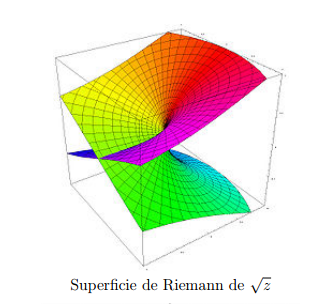
\includegraphics[scale=0.75]{img/supRiemann.png}
\end{center}

\begin{defn}[Superficie\IS de Riemann]
En geometría algebraica, una \textbf{superficie de Riemann} es una variedad compleja de dimensión (compleja) uno. Consecuentemente, la variedad real subyacente será de dimensión dos.

Una variedad real de dimensión 2 puede convertirse en una superficie de Riemann (frecuentemente de varios modos no equivalentes) si y sólo sí es orientable. De este modo, la esfera y el toro admitirán estructuras complejas, pero la banda de Möbius, la botella de Klein y el plano proyectivo real no.

Se sabe que la 2-esfera tiene una sola estructura analítica. Mientras que cada superficie orientable de género mayor que cero tiene una infinidad, contrastando con el punto de vista diferenciable ya que las superficies sólo tienen una estructura diferenciable.

Las superficies de Riemann constituyen el lugar natural donde estudiar el comportamiento global de numerosas funciones (por ejemplo $f(z)=\sqrt{z}$, $f(z)=\log(z)$).

El desarrollo de la idea de superficie de Riemann comenzó a mediados del siglo XIX de la mano del matemático Bernhard Riemann, con los intentos de extender el dominio de definición de funciones analíticas $\appl{f}{U}{C}$ definidas sobre un abierto U del plano complejo. La extensión maximal (extensión analítica) se lograba no sobre el propio plano complejo, sino sobre copias de abiertos del mismo que se solapaban, en lo que hoy día conocemos como variedad compleja de dimensión uno.

La \textbf{Superficie de Riemann} para $\sqrt[n]{z}$ es como la de $\sqrt{z}$ pero con $n$ copias del plano complejo en lugar de 2.
\end{defn}

Esta definición viene por cortesía de \href{http://es.wikipedia.org/wiki/Superficie_de_Riemann}{Wikipedia} pero no vamos a prestarle mucha atención, pues no lo estudiaremos durante este curso. Nos quedaremos con el primer método.

\begin{defn}[Rama\IS de una raíz]
\begin{itemize}
\item
Sea $\Omega$ un dominio en $\cplex$ y sea $\appl{g}{\Omega}{\cplex}$ una función continua tal que
\[\left(g(z)\right)^n=z \ \forall z \in \cplex\]
diremos que $g$ es una \textbf{rama de una raíz n-ésima de $z$ en $\Omega$}

\obs Las demás ramas son :
\[g_k(z)=g(z)\cdot e^{i\frac{2πk}{n}} \text{ con } k=1,2,..,n-1\]

\item
Sea $\appl{f}{Ω}{\cplex}$ y sea $\appl{F}{Ω}{\cplex}$ continua y tal que
\[\left( F(z)\right)^n=f(z) \ \forall z \in \cplex\]

Diremos que $F$ es una \textbf{rama de la raíz n-ésima de $f$}.

Más adelante veremos (usando el Teorema de Cauchy) que si $\appl{f}{Ω}{\cplex \setminus \{0\}}$ con Ω simplemente conexo, entonces tiene una raíz holomorfa en Ω y también un logaritmo holomorfo.
\end{itemize}
\end{defn}

\section{La función argumento}
Dado α $\in \real$ podemos definir una función \textbf{continua}
\[\appl{\psi}{Ω_α = \cplex \setminus \{re^{iα}: \ r \geq 0\}}{\real}\]
que nos lleva de un $z\in \cplex  \setminus \{re^{iα}: \ r \geq 0\}$ dado a su argumento en el intervalo $(α-2π,α)$, que denotamos como $arg_α(z)$.

La necesidad de quitar un radio viene del deseo de la que la función sea continua. Según por qué lado de la circunferencia nos acerquemos a ese radio, la imagen por $\psi$ tendería a α ó a 2π-α.

\newpage

\begin{defn}[Rama\IS del argumento]
Sea Ω un dominio en $\cplex$ y $\appl{f}{Ω}{\real}$ un función continua tal que
\[e^{if(z)}=\frac{z}{|z|}\]
diremos que $f$ es una rama del argumento de $z$ en Ω.

\obs Si $f_0$ es una rama del argumento de $z$ en Ω, entonces las demás ramas son de la forma $f_0+2πk$
\end{defn}
%TODO pedir apuntes en clase y revisar esta definición

Esta definición, como podemos observar, no es más que una mera extensión de la definición genérica de \textbf{rama de una función} dada en la segunda parte de la definición de \textbf{rama de una raíz}.

\begin{defn}[Rama\IS principal]
Llamaremos \textbf{Rama principal} a la función
\[\appl{Arg}{\cplex \setminus \{x \in \real: \ x\leq 0\}}{(-π,π)}\]
que, para cada punto complejo $z$ nos da el valor de su argumento contenido en $(-π, π)$
\end{defn}

\begin{defn}[Rama\IS de una función]
Sea $\appl{f}{Ω}{\cplex \setminus \{0\}}$ y sea $\appl{\psi}{Ω}{\real}$ continua tal que
\[e^{i \psi(z)} = \frac{f(z)}{|f(z)|} \ \forall z \in Ω\]
\end{defn}

\section{La función exponencial}
%TODO (DIBUJO EQUIVALENTE AL DE LA RAIZ)
La función exponencial es periódica con periodo 2πi
\begin{center}
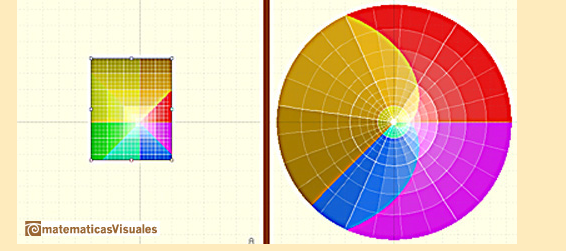
\includegraphics[scale=0.75]{img/exp1.png}
\end{center}

Cualquier banda horizontal del plano complejo de altura 2π se transforma en todo el plano complejo (con la excepción del origen)
\begin{center}
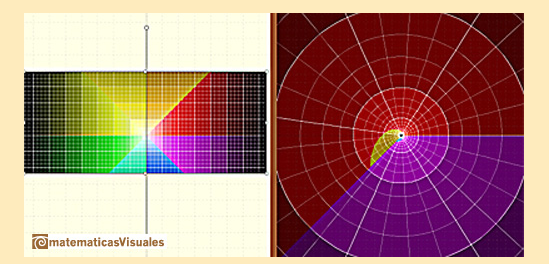
\includegraphics[scale=0.75]{img/exp2.png}
\end{center}

Dada una recta se transforma en una esperial, en una recta o en una circunferencia según la posición de la misma.
\begin{center}
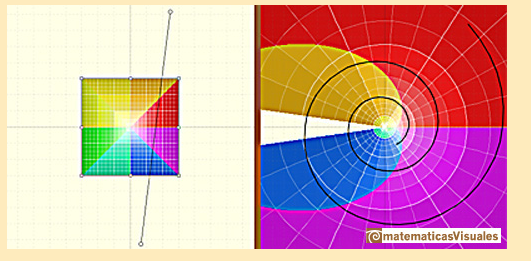
\includegraphics[scale=0.75]{img/exp3.png}
\end{center}

La fórmula de Euler
\[e^{iy}=\cos(y)+i\sin(y)\]
puede interpretarse como que la función exponencial enrolla el eje imaginario alrededor de la circunferencia unidad (Tristan Needham)
\begin{center}
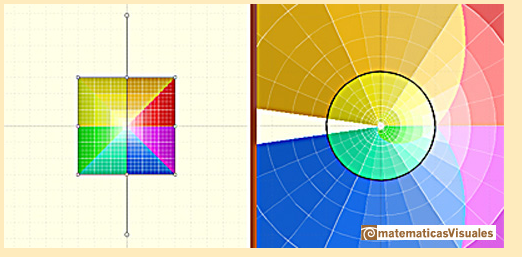
\includegraphics[scale=0.75]{img/exp4.png}
\end{center}

El semiplano a la izquierda del eje imaginario se mapea en el interior del círculo unidad, y el semiplano a la derecha del eje imaginario se mapea al exterior del círculo unidad.
\begin{center}
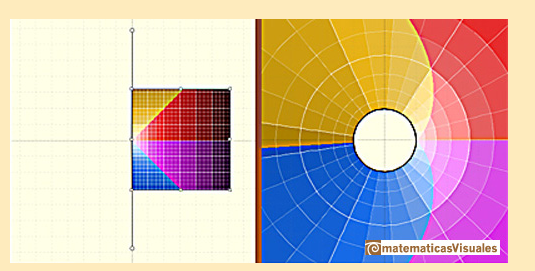
\includegraphics[scale=0.75]{img/exp5.png}
\end{center}

Las imágenes de cuadrados pequeños se asemejan a cuadrados y (en relación con esto) dos rectas que se intersecan se mapean en curvas que se intersecan con el mismo ángulo (Tristan Needham).

Ahora vamos a por el problema habitual: \textit{calcular la inversa}

La función $e^z$, de acuerdo a lo que acabamos de ver, sería inyectiva si nos restringimos a una banda horizontal de anchura 2π.

Sea $D_α=\{z \in \cplex : \ α < Im(z) < α+2π\}$, la función $\appl{g}{ω_α}{D_α}$ con $Ω_α = \cplex \setminus \{re^{iα} : \ r \geq 0\}$ definida por
\[g(w)=\log|w| + i\cdot arg_α(w)\]
es la inversa de $\appl{e^z}{D_α}{Ω_α}$

\newpage
\begin{defn}[Rama\IS de $\log(z)$]
Sea Ω un dominio en $\cplex$ y sea $\appl{g}{Ω}{\cplex}$ continua tal que $e^{g(z)}=z$ para todo $z \in Ω$ diremos que $g$ es una \textbf{rama de $\log(z)$ en Ω}
\end{defn}

\obs $0 \notin Ω$ pues $0 \in Ω \implies e^{g(0)}=0 !$

Llamaremos \textbf{la rama principal del $\log(z)$} a la función
\[\appl{\mop{Log}}{Ω_π}{\cplex}\]
definida por
\[\mop{Log}(z)=\log|z|+i\cdot \arg \footnote{Argumento principal, en $(-π,π)$} (z)\]

\obs Si $\log(z)$ es una rama del logaritmo de $z$ en Ω entonces es holomorfa, pues es la inversa de $e^z$ y $(e^z)'=e^z$ que siempre es no nula. Además $(\log(z))'=\frac{1}{z}$

\begin{lemma}
Sea $Ω \subset \cplex$ un dominio y sea $g_0$ una rama del logaritmo de $z$ en Ω, las demás ramas son de la forma $g_0+2πki$ con $k \in \ent$
\end{lemma}

\begin{proof}
Es claro que $h(z)=g_0(z)+2πki$ es una rama, pues es continua en Ω (ya que así lo es $g_0$).
\[e^{h(z)}=e^{g_0(z)+2πki}=e^{g_0(z)}e^{2πki}=e^{g_0(z)}=z \ \forall z \in Ω\]

Una vez hemos visto que las funciones de este tipo son ramas, nos queda ver que no hay más ramas posibles.

Sea $H(z)$ una rama. Precisamente por ser una rama sabemos que cumple:
\[e^{H(z)}=z=e^{g_0(z)} \ \forall z \in Ω\]
La única forma de que ocurra esto es que $H$ y $g$ difieran en un múltiplo de 2πi. Sabemos pues que
\[H(z)=g_0(z)+2k(z)πi\]
sólo nos queda probar que ese $k(z)$ no depende de $z$ y no se trata por tanto de una función sino de una constante.

Sea
\[G(z)=\frac{H(z)-g_0(z)}{2πi}\]
es continua y $G(Ω)\subset \ent$. Además, por ser continua mandará conexos en conexos y, puesto que en los enteros no hay más que puntos, la única posibilidad es que $G(Ω)$ sea un único punto, es decir, $k(z)=k$ independiente del punto.
\end{proof}

\begin{defn}[Rama\IS del $\log(f(z))$]
Sea $\appl{f}{Ω}{\cplex \setminus \{0\}}$ y se $\appl{F}{Ω}{\cplex}$ una función continua tal que
\[e^{F(z)}=f(z) \ \forall z \in Ω\]
diremos que $F$ es \textbf{rama del logaritmo de $f(z)$}.
\end{defn}

\obs Más adelante veremos que si Ω es simplemente conexo, podemos garantizar la existencia de esta $F$.

\section{Las potencias de z y las exponenciales con base a}
\begin{defn}[Rama\IS de $z^b$]
Sea $b \in \cplex$ y sea $\log(z)$ una rama del logaritmo en un dominio Ω. Entonces podemos definir la función
\[\appl{f}{Ω}{\cplex}\]
con
\[f(z)=e^{b\log(z)}\]
que se trata de una \textbf{rama de $z^b$}.
\end{defn}

\obs La $f$ anterior es holomorfa
\obs Dado $b \in \ent$, $f(z)$ no depende de la rama del logaritmo que tomemos, pues otra rama es $\log(z)+2kπi$ para algún $k \in \ent$
\[e^{b(\log(z)+2kπi)}=e^{\log(z)}e^{2kπbi} = e^{\log(z)}\]

Por todo esto podemos concluir que si $b \in \ent$ no hay diferentes ramas de $z^b$ en Ω.

Además, si $b \in \ent^+$ tenemos que
\[e^{b\log(z)}=\underbrace{e^{\log(z)}+\cdots + e^{\log(z)}}_{\text{b veces}}=z^b\]

\begin{defn}[Potencia\IS z de a]
Sea $a \in \cplex \setminus \{ 0 \}$ y sea $\log(a)$ un logaritmo de $a$, definimos la \textbf{potencia z de a} ($a^z$) a la función:
\[\appl{f}{\cplex}{\cplex}\]
con
\[f(z)=e^{z \log(a)}\]
\end{defn}

\obs La función $f$ definida anteriormente es holomorfa
\obs Dado $z=n \in \nat$, $f(z)=a^n$ es independiente del logaritmo de $a$ escogido, pues otro es de la forma $\log(a)+2kπi$ pero, como hemos visto anteriormente:
\[e^{n ( \log(a)+2πki)}=e^{n\log(a)}\]



\chapter{Fórmula integral de Cauchy y sus aplicaciones}

Sea $f(t)=u(t)+iv(t)$ una función continua $\appl{f}{[a,b]}{\cplex}$ definimos la \concept{Integral\IS} como:
\[\int_a^b f(t)\dif t = \int_a^bu(t)\dif t+i\int_a^bv(t)\dif t\]
siendo las dos integrales de la derecha integrales sobre los reales con las que ya sabemos trabajar.

\textbf{Propiedades}
\begin{enumerate}
\item $\displaystyle \int_a^b cf(t)\dif t=c\int_a^bf(t)\dif t$

\item $\displaystyle \left| \int_a^bf(t)\dif t \right| \leq \int_a^b |f(t)|\dif t$

\begin{proof}
Si $\int_a^bf(t)=0 \implies$ no hay nada que demostrar. Tenemos $0\leq 0$

Sea α$\in$ arg$\left(\int_a^bf(t)\dif t\right)$, tenemos que
\[\int_a^bf(t)\dif t=\left|\int_a^b f(t)\dif t \right| e^{iα}\footnote{Todo complejo puede expresarse como su módulo multiplicado por $e$ elevado a $i$ veces el argumento.}\]
multiplicando a ambos lados por $e^{-iα}$ tenemos:
\[\left| \int_a^bf(t)\dif t\right| \eqexpl{\footnote{A la izquierda tenemos un módulo, que es un número real, por lo que a la derecha deberemos tener otro. Por tanto coincide con su parte real.}} \mop{Re}  \left[ e^{-iα} \int_a^bf(t)\dif t\right] = \mop{Re}  \left[  \int_a^be^{-iα} f(t)\dif t\right] = \int_a^b \mop{Re} \left[ e^{-iα} f(t)\dif t\right]\]

\end{proof}
\end{enumerate}

\section{Fórmula de Green}
Antes de empezar, hagamos un breve bombardeo de definiciones y conceptos. Son bastante triviales pero resultarán muy importantes durante el desarrollo de este tema.

Una curva es una función continua $\appl{α}{[a,b]}{\cplex}$.

\begin{defn}[Curva\IS cerrada]
Si $α(a)=α(b)$ diremos que α es una \textbf{curva cerrada}.
\end{defn}


\begin{defn}[Curva\IS simple]
α es una curva simple si cumple la propiedad
\[\forall t_1,t_2 \in (a,b) \ α(t_1)=α(t_2) \implies t_1=t_2 \]

Es el ``equivalente'' a ser inyectiva.
\end{defn}

\begin{defn}[Curva\IS de Jordan]
Una curva \textbf{simple} y \textbf{cerrada} se llama \textbf{curva de Jordan}.
\end{defn}

Una curva $\appl{α}{[a,b]}{\cplex}$ es \concept[Diferenciable\IS a trozos]{diferenciable a trozos} si existe una partición de $[a,b]$:
\[a=t_0<t_1<\cdots < t_{n-1} < t_n=b\]
tal que α' existe en todos los intervalos $(t_i, t_{i+1})$ y se extiende a una función continua en $[t_i, t_{i+1}]$.

\begin{defn}[Longitud\IS de una curva]
La \textbf{longitud de una curva α} se define como:
\[\mop{long}(α)=\int_a^b | α'(t)| \dif t\]
\end{defn}

\begin{defn}[Camino]
Un camino es una curva diferenciable a trozos.
\end{defn}

\begin{example}
Si $\appl{α}{[a,b]}{\cplex}$ es un camino y β es monótona de $[c,d]$ a $[a,b]$, tenemos que
\[\mop{long} (α)=\mop{long} (α\circ β)\]

\textcolor{blue}{Completado por mi. No fiarse al 100\%}

Sabemos que
\[\mop{long} (α)=\int_a^b | α'(t)| \dif t\]
así que vamos a calcular la longitud de la composición:
\[\mop{long} (α \circ β) = \int_a^b |(α \circ β)'|\dif s = \int_a^b |β'(s) · α'(β(s))|\dif s=\int_a^b |β'(s)||α'(β(s))|\dif s\]

Sabiendo ahora que $β(s)=t$, derivamos y obtenemos: $β'(s)\dif s=\dif t$ y, al sustituirlo en la ecuación anterior, nos queda:
\[\mop{long} (α \circ β) = \int_a^bα(t)\dif t\]
\end{example}

Sea $\appl{α}{[a,b]}{\cplex}$ un camino y sea $\appl{f}{α([a,b])}{\cplex}$ una función continua, definimos la \concept{Integral\IS de línea}
\[\int_α f(z)\dif z = \int_a^bf(α(t))α'(t)\dif t\]
llamando $α(t)=x(t)+iy(t)$ y $f(α(t))=u(α(t))+iv(α(t))$ nos queda
\[\int_α f(z)\dif z = ... = \int_a^b\left(u(α(t))x'(t)-v(α(t))y'(t)\right)\dif t + i \int_a^b\left((u(α(t))y'(t)+v(α(t))x'(t) \right)\dif t\]
Con un poco de abuso de notación, podemos escribir:
\[\int_α f(z)\dif z=\int_α (udx-vdy) + i \int_α (udy+vdx)\]

\begin{example}
Dada la curva $α(t)=(1-t)+ti$ y la función $f(z)=z$ tenemos
\[\int_α f(z)\dif z = \int_0^1 ((1-t)+ti)(-1+i)\dif t = -\int_0^1\dif t + i \int_0^1(1-2t)\dif t\]

\end{example}

\begin{defn}[Integral\IS de línea respecto a la longitud de arco]
Definimos la \textbf{integral de línea respecto a la longitud de arco} como:
\[\int_α f(z)|\dif z| = \int_a^b f(α(t))|α'(t)|\dif t\]
\end{defn}

\begin{defn}[Curva\IS rectificable]
Una curva $\appl{a}{[a,b]}{\cplex}$ es \textbf{rectificable} si existe una constante $M>0$ tal que para cualquier partición $P=\{t_0,t_1,...t_n\}$ de $[a,b]$ se tiene que
\[V(α,P)=\sum_{k=1}^n\left|α(t_k)-α(t_{k-1})\right|<M\]
es decir, que tiene una longitud finita.

\obs
\[\mop{long} (α)=\sup\{V(α,P)\}\]
\end{defn}

\begin{lemma}
Todo camino es rectificable
\end{lemma}

Para α rectificable y $f$ continua en $α([a,b])$ existe la \concept{Integral\IS de Riemann-Stieldjes}
\[\int_a^bf(α(t))dα(t) = \int_αf(z)\dif z\]


\textbf{Propiedades de la integral de Riemann}


Sea $\appl{α}{[a,b]}{\cplex}$ un camino y sean $\appl{f,g}{α([a,b])}{\cplex}$ dos funciones continuas
\begin{enumerate}
\item Si $β$ es una función monótona, $C^1$ que manda el intervalo $[c,d]$ en $[a,b]$ con $β(c)=a$ y $β(d)=b$, entonces:
\[\int_α f(z)\dif z = \int_{α \circ β} f(z)\dif z\]
es decir, \textbf{la integral de línea es independiente de la parametrización}.

\obs Si $β(c)=b$ y $β(d)=a$
\[\int_α f(z)\dif z = -\int_{α \circ β} f(z)\dif z\]

\item Para todo $a,b \in \cplex$
\[\int_α(af+bg)\dif z = a \int_α f\dif z + b \int_α g\dif z\]

\item Si $c \in [a,b]$ y definimos $α_1(t)=α(t) \ \forall  t \in [a,b]$ y $α_2(t)=α(t) \ \forall t \in [c,d]$ tenemos
\[\int_α f(z)\dif z = \int_{α_1}f(z)\dif z + \int_{α_2}f(z)\dif z \]

\item
\[\left| \int_α f(z)\dif z \right| \leq \int_α |f(z)||\dif z| \leq \sup_{z \in α([a,b])} \left( |f(z)|\right)\mop{long} (α)\]

\item Si $\{f_n\}$ es una sucesión de funciones continuas en $α([a,b])$ que convergen uniformemente a $f$, entonces
\[\int_α f_n(z)\dif z \longrightarrow \int_α f(z)\dif z\]

\item Si $f$ está definida en un entorno de $α([a,b])$ y allí tiene primitiva, entonces
\[\int_α f(z)\dif z = F(α(b))-F(α(a))\]
en particular, si α es cerrada esta vale 0.
\end{enumerate}

\newpage
Procedamos a demostrar algunas de estas propiedades:
\begin{proof}
\begin{enumerate}
\item
\[\int_{α \circ β}f(z)\dif z = \int_c^df((α \circ β)(s))(α\circ β)'ds = \int_c^df((α \circ β)(s)) α'(β(s))β'(s)ds =\]
\[= \int_a^b f(α(t))α'(t)=\int_α f(z)\dif z\]

\item[4]
Ya vimos que si $\appl{F}{[a,b]}{\cplex}$ continua, teníamos que
\[\left| \int_a^bF(t)\dif t\right| \leq \int_a^b|F(t)|\dif t\]
Por tanto
\begin{multline*}
\left| \int_α f(z)\dif z\right| = \left| \int_a^bf(α(t))α'(t)\dif t\right| l\leq \int_a^b |f(α(t))||α'(t)|\dif t \leq \\ \leq \sup_{z \in α([a,b])}|f(z)|\int_a^b|α'(t)|\dif t= \sup_{z \in α([a,b])}(|f(z)|)\mop{long} (α)
\end{multline*}

\item[5]
\[\left| \int_α f_n\dif z - \int_α f \dif z\right| = \left| \int_α(f_n(z)-f(z))\dif z\right| \leq \int_α |f_n(z)-f(z)||\dif z| \leq\]
\[\leq \sup_{z \int α([a,b])} |f_n(z)-f(z)|\mop{long} (α)\]

Puesto que tenemos convergencia uniforme, sabemos que
\[ \sup_{z \int α([a,b])} |f_n(z)-f(z)| < ε\]
para un n grande, por lo que
\[\forall ε \ \exists N \tq \forall n > N \left| \int_α f_n\dif z - \int_α f \dif z\right| < ε\]

\item[6]
\[\int_α f(z)\dif z = \int_α F'(z)\dif z = \int_a^bF'(α(t))α'(t)=\int_a^b \frac{d}{\dif t}(F \circ α)(t)\dif t \eqexpl{\text{F=G+iH}} \]
\[= \int_a^b\frac{d}{\dif t} (G \circ α)(t)\dif t + i\int_a^b\frac{d}{\dif t}(H \circ α)(t)\dif t \eqexpl{T.F.C} \]
\[ = (G\circ α)(b)-(G \circ α)(b) + i\left( (H\circ α)(b)-(H \circ α)(b)\right) = (F \circ α)(b)-(F \circ α)(a)\]
\end{enumerate}
\end{proof}

\newpage

\begin{example}
Vamos a calcular
\[\int_{|z|=1}  \frac{1}{z} \dif z\]

Vamos a calcularlo de dos formas distintas:
\begin{itemize}
\item Aplicamos directamente la definición

Primero parametrizamos la curva sobre la que estamos integrando (circunferencia unidad).

Es sencillo ver que $α(t)=\cos t + i \sin t = e^{it}$ y $α'(t)=ie^{it}$

Procedemos ahora a calcular la integral con lo visto anteriormente:
\[\int_{|z|=1}  \frac{1}{z} \dif z = \int_0^{2π}\frac{1}{e^{it}}ie^{it}\dif t = 2πi\]

\item Dividimos la curva en dos trozos y empleamos dos ramas del logaritmo.
\textbf{Se deja como ejercicio para el lector}
\end{itemize}
\end{example}

\section{Teorema de Cauchy}

Antes de empezar, debemos recordar el \textbf{Teorema de Green}

\begin{theorem}[Teorema\IS de Green]
Sea $\appl{α}{[a,b]}{\real^2}$ un camino simple y cerrado en $\real^2$; Ω, el interior de α y $\appl{P, Q}{\real^2}{\real}$, dos funciones continuas en $Ω \cup (α([a,b]))$ y $C^1$ en Ω, entonces
\[\int_α P\dif x+Q \dif y = \iint_Ω \left( \deriv{Q}{x}-\deriv{P}{y}\right) \dif x\dif y\]
\end{theorem}

\begin{theorem}[Teorema\IS de Cauchy]
Sea $f=u+iv$, una función holomorfa en Ω con f' continua en Ω, y sea α un camino simple y cerrado, se cumple que:
\[\int_α f(z)\dif z = \int_α u\dif x-v\dif y+i\int_α v\dif x+u\dif y \eqexpl{\text{Green}}\]
\[\eqexpl{\text{Green}} -\iint_Ω (v_x+u_y)\dif x \dif y + i \iint_Ω (u_x-v_y)\dif x \dif y = 2i \iint_Ω \od{f}{\bar{z}}\dif x \dif y = 0\]
\end{theorem}

\begin{theorem}[Teorema\IS de Cauchy-Goursat]
Sea $f$ holomorfa en un dominio Ω $\subset \cplex$ y sea $R$ un rectángulo contenido en Ω entonces
\[\int_{\partial R} f(z)\dif z = 0\]
donde $\partial R$ es la frontera del rectángulo.
\end{theorem}

\begin{proof}

Para empezar escribimos el rectángulo de la siguiente forma
\[R = \{x+iy \tq a \leq x \leq b, \ c \leq y \leq d\}=[a,b]\times[c,d]\]

Dividimos ahora el rectángulo en cuatro rectángulos iguales: $R^{(i)}$ con $i=1,2,3,4$ y orientamos todos estos rectángulos en sentido antihorario.

Ahora procedemos a calcular la integral mencionada en el teorema:
\[\int_{\partial R}f(z)\dif z = \int_{\partial R^{(1)}}f(z)\dif z+\int_{\partial R^{(2)}}f(z)\dif z+\int_{\partial R^{(3)}}f(z)\dif z+\int_{\partial R^{(4)}}f(z)\dif z \implies\]

\[\implies \left| \int_{\partial R}f(z)\dif z\right| \leq \sum_{i=1}^4 \left|\int_{\partial R^{(i)}}f(z)\dif z \right|\]
y sabemos que al menos hay un $R^{(i)}$ que cumple la condición:
\[\left| \int_{\partial R^{(i)}}f(z)\dif z\right| \geq \frac{1}{4} \left| \int_{\partial R}f(z)\dif z\right| \]
ya que en caso de ser todas las integrales menores que 1/4 de la suma tendríamos que nunca alcanzarían el valor y nos quedaría una desigualdad estricta.

Sin pérdida de generalidad podemos suponer que el rectángulo que satisface esta condición es $R^{(1)}$.

Ahora dividimos este rectángulo en 4 rectángulos iguales y repetimos este proceso.

Según vamos repitiendo este proceso generamos una sucesión decreciente de rectángulos $\{R_n\}$ tales que
\[\left| \int_{\partial R_n}f(z)\dif z\right| \geq \frac{1}{4} \left| \int_{\partial R_{n-1}}f(z)\dif z\right| \]

Por tanto, tenemos que
\[\left| \int_{\partial R_n}f(z)\dif z\right| \geq \frac{1}{4^n} \left| \int_{\partial R}f(z)\dif z\right| \implies 4^n\left| \int_{\partial R_n}f(z)\dif z\right| \geq\left| \int_{\partial R}f(z)\dif z\right|\]

Sea $z^*$ el punto en $\bigcap_{n=1}^{\infty}R_n$, dado ε > 0 $\exists δ > 0 \tq$
\[|z-z^*| < δ \implies \left| \frac{f(z)-f(z^*)}{z-z^*}-f'(z^*)\right| < ε\]

Si tomamos un $n$ suficientemente grande como para que
\[R_n\subset \{z \tq |z-z^*|<δ\}\]
entonces para todo $z\in R_n$ se cumple que
\[\left| f(z)-f(z^*)-f'(z^*)(z-z^*)\right| < ε|z-z^*|\]

Podemos ver que
\[\left| \int_α f(z)\dif z\right| =\footnote{$\int_α f(z^*) = 0$  por ser curva cerrada } \left| (f(z)-f(z^*)-f'(z^*)(z-z^*)\right| \leq \int_{\partial R_n} | (f(z)-f(z^*)-f'(z^*)(z-z^*)||\dif z| \leq\]
\[\leq \int_{\partial R_n}ε|z-z^*||\dif z| \leq ε \int_{\partial R_n}\text{diam}(R_n)|\dif z|=ε\text{diam}(R_n)\text{long}(\partial R_n) = ε \frac{1}{2^n}\text{diam}(R)\frac{1}{2^n}\text{long}(\partial R) \]

%TODO cambiar eso por una referencia:
Aplicando esta desigualdad a
\[4^n\left| \int_{\partial R_n}f(z)\dif z\right| \geq\left| \int_{\partial R}f(z)\dif z\right|\]
llegamos a
\[\left| \int_{\partial R}f(z)\dif z\right| \leq 4^n\left| \int_{\partial R_n}f(z)\dif z\right| \leq 4^nε \frac{1}{2^n}\text{diam}(R)\frac{1}{2^n}\text{long}(\partial R) =ε \text{diam}(R)\text{long}(\partial R)\]
y vemos que, por ser ε arbitrario,
\[\int_{\partial R}f(z)\dif z=0\]
\end{proof}

\begin{theorem}
Sea Ω un dominio en $\cplex$, R un rectángulo en Ω y $\{z_i\}$ un conjunto finito de puntos en el interior de R tenemos que:

Si $f$ es holomorfa en Ω$\setminus \{z_i\}$ y
\[\lim_{z \to z_i}(z-z_i)f(z)=0 \ \forall i\]
entonces
\[\int_{\partial R}f(z)\dif z=0\]
\end{theorem}
\begin{proof}
Para demostrar que el teorema es cierto basta con demostrarlo con un conjunto formado por un único punto. Una vez que veamos que ese punto no molesta para el cálculo de la integral, podremos extender la idea a un conjunto finito de puntos.

Tenemos el punto $z_0$, contenido en el rectángulo y en el que la función no es holomorfa. Dado ε > 0, vamos a dividir el rectángulo en 9 \textit{rectangulitos} de forma que el rectángulo central sea un cuadrado centrado en $z_0$ y
\[|(z-z_0)f(z)|<ε \ \forall z \in \partial R_0\]
siendo $R_0$ el cuadrado central que contiene al punto $z_0$.

Como $\int_{\partial R}f(z)\dif z =\footnote{Por el teorema de Cauchy sabemos que en el resto de rectángulos la integral es 0, pues $f$ es holomorfa} \int_{\partial R_0}f(z)\dif z$

Con lo que acabamos de ver, tenemos:
\[\left| \int_{\partial R} f(z)\dif z\right|= \left| \int_{\partial R_0} f(z)\dif z\right| \leq  \int_{\partial R} |f(z)||\dif z| \leq \int_{\partial R_0} \frac{ε}{|z-z_0||\dif z|} \leq\footnote{Siendo $l_0$ el lado del rectángulo $R_0$ vemos que $|z-z_0|\geq \frac{1}{2}l_0$} \frac{2ε}{l_0}4l_0 = 8ε\]
con lo que hemos vuelto a ver que es menor que cualquier valor, por tanto el valor absoluto de esta integral vale 0.
\end{proof}

\begin{theorem}
Si $f(z)$ es holomorfa en $\{z: \ |z-z_0|<r\} \implies$ existe $F$ holomorfa en $\{z: \ |z-z_0|<r\}$ tal que $F'=f$
\end{theorem}
\begin{proof}
Siendo $z=z+iy$ y $z_0=x_0+iy_0$, definimos $α_z$ como el camino formado por dos segmentos perpendiculares que une un punto con el otro.

Definimos
\[F(z)=\int_{α_z}f(z)\dif z =\int_{x_0}^xf(t+iy_0)\dif t+i \int_{y_0}^yf(x+it)\dif t\]

Ahora, si $α_z$ era el camino que unía $z_0$ con $z$, definimos ahora el camino β que consiste en unir $α_z$ con el camino de retorno. Este camino β forma un rectángulo teniendo que $z$ y $z_0$ en vértices opuestos.

Por tratarse de un camino cerrado sabemos que la integral será 0, de modo que
\[0 = \int_βf(z)\dif z = \int_{α_z}f(z)\dif z-\int_{\bar{α_z}}f(z)\dif z\]
siendo $\bar{α_z}$ el camino que va de $z_0$ a $z$ siguiendo el camino que establecimos como retorno, pero en sentido contrario.

Por tanto estamos obteniendo que la integral es la misma con independencia del camino seguido para unir $z_0$ con $z$.

Así que podemos definir también
\[F(z)=\int_{\bar{α_z}}f(z)\dif z =i\int_{y_0}^yf(x_0+it)\dif t + \int_{x_0}^xf(t+iy)\dif t\]

Ahora queremos ver que esta $F(z)$ que hemos definido es holomorfa. Para confirmarlo vamos a ver que cumple las ecuaciones de Cauchy-Riemann.

Basándonos en la primera definición de $F(z)$ tenemos:
\[F_y(z) = i \frac{\partial}{\partial y} \int_{y_0}^yf(x+it)\dif t \eqexpl{T.F.C.} i f(x+iy)=if(z)\]

para calcular ahora la derivada respecto de $x$ nos basamos en la segunda definición:
\[F_x(z)=f(x+iy)=f(z)\]

Combinando ambas ecuaciones obtenemos que
\[F_x(z)=f(z)=-iF_y(z)\]
que son las ecuaciones de Cauchy-Riemann. Además $F'(z)=F_x(z)=f(z)$ y $f$ es continua. Por tanto podemos afirmar que $F(z)$ es holomorfa en $|z-z_0| < r$
\end{proof}

\begin{theorem}[Teorema\IS de Cauchy en el disco]
Si $f$ es holomorfa en $\{z: \ |z-z_0|<r\} \implies \int_α f(z)\dif z = 0$ para todo camino cerrado α en $\{z: \ |z-z_0|<r\}$
\end{theorem}
\begin{proof}
Por el teorema anterior sabemos que existe $F$ holomorfa tal que $F'=f$ en $\{z: \ |z-z_0|<r\}$.

Por el teorema fundamental sabemos que
\[\int_α f(z)dx = F(b)-F(a)\]
pero como $a=b$ por tratarse de un camino cerrado, tenemos que la integral vale 0
\end{proof}

\newpage

\begin{example}
S $f$ es holomorfa en $\{z: \ |z-z_0|<r\}$ menos en un conjunto finito de puntos $\{z_1, z_2, ... , z_s\}$ en los que
\[\lim_{z \to z_j} (z-z_j)f(z)=0 \ \forall j=1,2,...,s\]
entonces la integral sobre un camino cerrado es 0.

\textbf{Este ejercicio se deja para el lector}
\end{example}

Vamos a ver a continuación una versión más extensa del \textbf{Teorema de Cauchy en el disco}. Para ello necesitamos ver antes una definición:

\begin{defn}[{Í}ndice\IS de un punto con respecto a un camino cerrado]
Sea $\appl{α}{[z,b]}{\cplex}$ un camino cerrado y sea $z_0 \in \cplex \setminus α([a,b])$, el \textbf{índice del punto con respecto a  α} se define como:
\[Ind_α(z_0)=\frac{\arg (α(b)-z_0)-\arg (α(a)-z_0)}{2π}\]
donde $\arg (α(t)-z_0)$ es una rama del argumento de $α(t)-z_0$

Este índice mide el número de vueltas que da la curva alrededor del punto teniendo en cuenta el sentido de giro.
\end{defn}

\obs Sea $β(t)=α(t)-z_0$ una función $\appl{β}{[a,b]}{\cplex}$, una rama del argumento de β será una función continua $g$, definida sobre el mismo dominio $\appl{g}{[a,b]}{\cplex}$ y que represente el ángulo, es decir,
\[e^{ig(t)}=\frac{β(t)}{|β(t)|}\]

\textbf{Importante:}
Recordamos que cuando estudiamos la rama del argumento, si tomábamos una curva cerrada que encerrara el origen veíamos que el ángulo crecía de 0 a 2π para acabar valiendo 0 al final, con lo que ya no era continua, puesto que nos estábamos acercando al punto inicial pero la imagen no se acercaba.

Ahora este problema no existe pues no volvemos realmente al mismo punto sino que nos movemos desde $α(a)$ hasta $α(b)$, que no son el mismo punto.

\textbf{La clave reside en que estamos tomando como dominio el intervalo $[a,b]$ en lugar del grafo de la curva.}

\textbf{No es lo mismo $\appl{g}{[a,b]}{\cplex}$ que $\appl{g}{Ω}{\cplex}$, siendo Ω el grafo de la curva α, $Ω \subset \cplex$}

\begin{example}
Sea $\appl{α}{[0,1]}{\cplex}$ con $α(t)=e^{2πit}$, tenemos:
\[\cind_α(0)=\frac{2π-0}{2π}=1\]
\[\cind_α(2)=\frac{π - π}{2π}=0\]

Sea ahora $\appl{α}{[0,1]}{\cplex}$ con $α(t)=e^{4πit}$, tenemos:
\[\cind_α(0)=\frac{4π-0}{2π}=2 \]
\end{example}

Otra forma de calcular este índice sería:
\[\cind_α(z_0) = \frac{1}{2π i}\int_α \frac{\dif z}{z-z_0}\]

Si $\arg(α(t)-z_0)$ es una rama del argumento de $α(t)-z_0$, entonces
\[\log(α(t)-z_0)=\log|α(t)-z_0|+ i \arg (α(t)-z_0)\]
es una rama del logaritmo de $α(t)-z_0$ y se tiene que
\[\cind_α(z_0)= \frac{ \log(α(b)-z_0)-\log(α(a)-z_0)}{2πi}\]

Vamos a buscar ahora esa rama de $\log(α(t)-z_0)$.

Ya sabemos que si $\appl{F}{[a,b]}{\cplex}$ es una rama del logaritmo de $α(t)-z_0$ entonces es continua y cumple:
\[e^{F(t)} = α(t)-z_0\]
derivando formalmente\footnote{No sabemos si la función existe y por tanto no sabemos si será diferenciable. Suponemos que si que lo es y ya veremos luego qué pasa.}
\[e^{F(t)}F'(t) = α'(t) \implies F'(t)=\frac{α'(t)}{α(t)-z_0}\]
por tanto, en caso de que existiera esta $F(t)$ de la que estamos hablando tendríamos:
\[F(t)=\int_a^t \frac{α'(t)}{α(t)-z_0}\dif t +c_1\]
con $c_1$ una constante tal que $e^{c_1}=α(t)-z_0$ puesto que queremos que se cumpla $e^{F(a)}=α(t)-z_0$

Tenemos que $F(t)$ es continua en $[a,b]$ y diferenciable en los mismos puntos que α siendo su derivada conocida.

Queremos probar que
\[(α(t)-z_0)e^{-F(t)}=1\]

Para ello definimos $\Psi(t)=(α(t)-z_0)e^{-F(t)}$ y derivando llegamos a
\[\psi'(t)=α'(t)e^{-F(t)}+(α(t)-z_0)e^{-F(t)}\cdot F'(t)=0\]
pudiendo hacer esta derivada en aquellos puntos donde exista la derivada de α. Si sustituimos $F'(t)$ por su valor calculado anteriormente vemos que, efectivamente la derivada es 0, por lo que $\Psi(t)$ es constante.

Ahora queremos garantizar que esa constante es 1. Para ello estudiamos el valor de $\Psi(t)$ en un punto:
\[\Psi(a)=(α(a)-z_0)e^{-F(a)}=(α(a)-z_0)\frac{1}{(α(a)-z_0)}=1\]
por lo que queda probado que $\Psi(t)$ es constante igual a 1.

$F$ es rama del logaritmo de $α(t)-z_0$ y obtenemos:
\[\cind_α(z_0) = \frac{F(b)-F(a)}{2πi}=\frac{1}{2πi}\int_a^b \frac{α'(t)}{α(t)-z_0}\dif t=\frac{1}{2πi}\int_α \frac{\dif z}{z-z_0}\]

\begin{theorem}[Fórmula integral de Cauchy en el disco]
Sea $f$ una función holomorfa en $\{z \tq |z-z_0| < r\}$ y sea α un camino cerrado en el disco. Entonces
\[\cind_α(z_0)f(z)=\frac{1}{2πi}\int_α \frac{f(w)}{w-z}\dif w \; \forall z \notin α\]

\end{theorem}
\begin{proof}
Sea
\[F(w)=\frac{f(w)-f(z)}{w-z}, \text{ holomorfa para todo } w \neq z\]
tenemos que
\[(w-z)F(w)=f(w)-f(z) \to 0 \text{ cuando } w \to 0\]

Entonces por el teorema de Cauchy en el disco tenemos que
\[0 = \int_α F(w)\dif w = \int_α \frac{f(w)-f(z)}{w-z} \dif w = \int_α \frac{f(w)}{w-z}\dif w-f(z) \underbrace{\int_α\frac{\dif w}{w-z}}_{2πi\cdot \cind_α(z)}\]
y despejando llegamos a la igualdad que queríamos probar.
\end{proof}

\begin{example}
Tomemos la función
\[f(z)=\frac{1}{2πi}\int_{w: \ |w-z|=r}\frac{f(w)}{w-z}=\frac{1}{2πi}\int_0^{2π}\frac{f(z+re^{it})}{re^{it}}re^{it}i\dif t\]
Para obtener la última integral hemos realizado un cambio de variable siendo $w=z+re^{it}$

Tras simplificar en la última integral llegamos a:
\[f(z)=\frac{1}{2π}\int_0^{2π}f(z+re^{it})\dif t\]

\end{example}
\obs En definitiva, esta fórmula nos está diciendo que el valor de la función holomorfa en un punto $z$ se calcula como media de los valores de la función en los puntos que lo rodean.


\begin{prop}
Sea $\appl{α}{[a,b]}{\cplex}$ un camino cerrado y $\appl{\Psi}{α([a,b])}{\cplex}$ continua, entonces
\[f(z)=\frac{1}{2πi}\int_α \frac{\Psi(w)}{w-z}\dif w \ \forall z \notin α([a,b])\]
es analítica (y por tanto holomorfa) y se cumple que
\[f^{(n)}(z) = \frac{n!}{2πi}\int_α \frac{\Psi(w)}{(w-z)^{(n+1)}}\dif w \ \forall n \in \nat\]
\end{prop}

\begin{proof}
Sea $z_0 \notin α([a,b])$ y sea $r=\text{dist}(z_0, α([a,b]))$, para cada $z$ tal que $|z-z_0|<r$ tenemos
\[2πif(z)=\int_α \frac{\Psi(w)}{w-z}\dif w\]

Podemos ver que
\[\frac{1}{w-z} =\frac{z-z_0}{1-\left( \frac{z-z_0}{w-z_0}\right)}\dif w\]
y sabemos que
\[\frac{1}{1-\frac{z-z_0}{w-z_0}} =\footnote{Ocurre sólo si la razón es menor que 1 en valor absoluto, es decir, $|z-z_0|<|w-z_0|$, que sabemos es cierto.} \sum_n \left( \frac{z-z_0}{w-z_0}\right)^n\]

Si aplicamos estas dos ecuaciones en la integral que define $f$ tenemos:
\[2πif(z)= \int_α \frac{\Psi(w)}{w-z_0}\frac{1}{1-\left( \frac{z-z_0}{w-z_0}\right)}\dif w\]

Puesto que
\[g_N(z)=\frac{\Psi(w)}{w-z_0}\sum_{n=0}^N\left(\frac{z-z_0}{w-z_0}\right)^n\]
converge uniformemente en $|z-z_0| < |w-z_0|$

\[g_N(z) \rightrightarrows g(w)=\frac{\Psi(w)}{w-z_0}\frac{1}{1-\left( \frac{z-z_0}{w-z_0}\right)}\]

Por tanto
\[\int_α g(w)\dif w = \lim_{N \to \infty} \int_α f_N(w)\dif w = \lim_{N \to \infty} \int_α \frac{\Psi(w)}{w-z_0}\sum_{n=0}^N\left(\frac{z-z_0}{w-z_0}\right)^n = \]
\[= \lim_{N \to \infty}\sum_{n=0}^{\infty} \int_α \frac{\Psi(w)}{(w-z_0)^{n+1}}\dif w(z-z_0)^n = \sum_{n=0}^{\infty} \left[\int_α \frac{\Psi(w)}{(w-z_0)^{n+1}}\right] (z-z_0)^n\]

Por tanto
\[f(z)=\sum_{n=0}^{\infty} \left(\frac{1}{2πi}\int_α \frac{\Psi(w)}{(w-z_0)^{n+1}}\right)\dif w(z-z_0)^n\]
con lo que ya tenemos el desarrollo de $f$ en serie de potencias de $|z-z_0|$. Por tanto $f$ es analítica.

Además
\[a_n=\frac{1}{n!}f^{(n)}(z_0) \implies f^{(n)}(z_0) = \frac{n!}{2πi}\int_α \frac{\Psi(w)}{(w-z)^{n+1)}}\dif w\]
\end{proof}

\subsection{Equivalencia entre holomorfía y analiticidad}
\begin{theorem}
Sea $f$ holomorfa en un abierto $Ω \subset \cplex$ entonces:
\begin{enumerate}
\item $f$ es analítica en Ω

\item Existen todas las derivadas de $f$ y son holomorfas en Ω
\end{enumerate}
\end{theorem}

\begin{proof}
Sea $z \in Ω$ con $B(z,r)=\{w : \ |w-z| < r\} \subset Ω$.

Por la fórmula integral de Cauchy para $α \in \partial B(z, \frac{r}{2})$ se tiene
\[f(z)=\frac{1}{2πi}\int_α \frac{f(w)}{w-z} \dif w\footnote{Consideramos α tal que sólo de una vuelta en torno a z de modo que el índice sea 1.}\]
que es anaĺítica por la proposición y además
\[f^{(n)}(z)=\frac{n!}{2πi} \int_α \frac{f(w)}{(w-z)^{n+1}} \dif w\]
siendo todas estas derivadas holomorfas.

Por tanto tenemos que si una función es holomorfa será analítica y, puesto que ya habíamos visto la implicación opuesta, podemos afirmar que
\[\text{holomorfa} \iff \text{analítica}\]
\end{proof}

\begin{theorem}[Singularidad\IS evitable]
Sea Ω un abierto en $\cplex$ y $z_0 \in \cplex$. Si $\appl{f}{Ω \setminus \{z_0\}}{\cplex}$ es holomorfa y $\lim_{z \to z_0} (z-z_0)f(z) = 0$ entonces $f$ puede extenderse a una función holomorfa en Ω.
\end{theorem}
\begin{proof}
Supongamos $z_0 = 0$ (en caso de no ser así podríamos tomar $g(z)=f(z+z_0)$).

Sea $R$ un rectángulo que contiene al origen en su interior, fijamos un punto $z$ del interior de $R$ y distinto del origen.

Definimos
\[F(w)=\frac{f(w)-f(z)}{w-z}\]
holomorfa en $Ω \setminus \{0, z\}$.

Además $(w-z)F(w)=f(w)-f(z)$ converge a 0 cuando nos acercamos a z. Por tanto,
\[wF(w)=\frac{f(w)-f(z)}{w-z} w\to 0 \text{ cuando w $\to 0$}\]
puesto que $wF(w) \to 0$ cuando $w \to 0$.

Por el teorema de Cauchy sobre rectángulos tenemos que
\[0 = \int_{\partial R}F(w)\dif w  = \int_{\partial R} \frac{f(w)-f(z)}{w-z}  \dif w =  \int_{\partial R}\frac{f(w)}{w-z} -\int_{\partial R} \frac{1}{w-z}\dif w \implies\]

\[\implies f(z)=\frac{1}{2πi} \int_{\partial R} \frac{f(w)}{w-z}\dif w \ \forall z \in R \setminus \{0\}\]

Por tanto, una extensión holomorfa de $f$ es
\[g(z)=\left\{ \begin{array}{lcc}
             f(z) &   si  & z \in Ω \setminus \{0\}\\
             \\ \frac{1}{2πi} \int_{\partial R} \frac{f(w)}{w-z}\dif w &  si  & z\in R
             \end{array}
   \right.\]
\end{proof}

\begin{lemma}
Si $f$ es holomorfa en Ω y $f(z_0)=f'(z_0)=f''(z_0)=...=f^{(k-1)}(z_0)=0$, entonces $f(z)=(z-z_0)^kg(z)$ con $g$ holomorfa en Ω.
\end{lemma}
\begin{proof}
Sea
\[h_1(z)=\frac{f(z)}{z-z_0}\]
holomorfa en $Ω\setminus \{z_0\}$, tenemos que
\[\lim_{z \to z_0} (z-z_0)h_1(z)=\lim_{z \to z_0} f(z)=f(z_0)=0\]
lo que implica que $h_1$ se extiende a una función holomorfa en Ω y, por continuidad, se cumple:
\[h_1(z_0)=\lim_{z \to z_0} h_1(z)=\lim_{z \to z_0}\frac{f(z)-f(z_0)}{z-z_0}=f'(z_0)\]

Tenemos ya $f(z)=(z-z_0)h_1(z)$ con $h_1$ holomorfa en Ω y $h_1(z_0)=0$

Queremos seguir sacando factores de la forma $(z-z_0)$ para llegar al resultado que queremos demostrar, de modo que repetimos el procedimiento anterior con esta $h_1$.

Definimos
\[h_2(z) = \frac{h_1(z)}{z-z_0}\]
holomorfa en $Ω\setminus \{z_0\}$. pero $(z-z_0)h_2(z)=h_1(z) \rightarrow h_1(z_0)=f'(z_0)$.

Por tanto, puedo extender $h_2$ a una función holomorfa en Ω y, además,
\[h_2(z_0) = \lim_{z \to z_0}h_2(z=\lim_{z \to z_0}\frac{h_1(z)-h_1(z_0)}{z-z_0}=h_1'(z_0)=f''(z_0)\]
y tenemos que
\[f(z)=(z-z_0)^2h_2(z)\]

Finalmente obtenemos $f(z)=(z-z_0)^k g(z)$
\end{proof}

Básicamente estamos tomando una función cuyo desarrollo de Taylor tiene $a_i=0$ para los primeros k-1 coeficientes. Lo que queda a partir del $a_k$ es la función $g(z)$.

Técnicamente este resultado es algo más general que eso, pues es un resultado global mientras que el polinomio de Taylor es local.

\section{Teorema de Morera}

\begin{theorem}
Sea $\appl{f}{Ω}{\cplex}$ continua con Ω un abierto, si para todo $z \in Ω$ existe un disco $B(z,r_z)=\{w : |w-z|<r_z\}\subset Ω$ tal que
\[\int_{\partial R}f(z)\dif z=0\]
para todos los rectángulos $R \subset B(z,r_z)$, entonces $f$ es holomorfa Ω
\end{theorem}

\begin{proof}
Esta demostración se deja como ejercicio para el lector.

La idea consiste en emplear el Teorema de Cauchy para obtener la función primitiva, que será holomorfa.
\end{proof}

\section{La función primitiva en un dominio simplemente conexo}
\subsection{Teoremas de Cauchy para dominios simplemente conexos}

Recordemos que un dominio simplemente conexo es aquel que ``no tiene huecos''. Es decir, toda curva cerrada se puede contraer a un punto.

\begin{defn}[Dominio\IS simplemente conexo]
Un dominio (abierto y conexo) en $\cplex$ es simplemente conexo si y sólo si su complementario en $\widehat{\cplex}$ es conexo
\end{defn}

\begin{example}
El interior de una circunferencia en $\cplex$ es simplemente conexo pues su complementario es el resto del plano junto con el infinito. Puesto que el plano se extiende hasta el infinito, resulta ser conexo.

Sin embargo, si tomamos el exterior de la circunferencia, su complementario es la circunferencia más el infinito que deja de ser conexo, pues no podemos conectar el infinito con la circunferencia sin pasar por el plano.
\end{example}

\obs Un dominio Ω es simplemente conexo si y sólo si el índice es 0 para todo punto y todo camino cerrado en el dominio.

\begin{theorem}[Teorema\IS de Cauchy] Si $f$ es holomorfa en Ω, siendo Ω un dominio simplemente conexo, entonces \[ \int_α f(z)\dif z=0 \] para todo camino cerrado α en Ω.
\end{theorem}

\subsection{Fórmula integral de Cauchy}
Si $f$ es holomorfa en Ω, siendo Ω un dominio simplemente conexo y α un camino cerrado en Ω se cumple que
\[\cind_α(z)f^{(n)}(z) = \frac{n!}{2πi}\int_α \frac{f(w)}{(w-z)^{n+1}}\dif w \ \forall z \notin α \text{ con } n= 1,2,3,...\]

\begin{proof}[Teorema de Cauchy para dominios simplemente conexos]

Esta demostración queda como ejercicio para el lector aunque vamos a dar algunas ideas de la misma.

\begin{enumerate}
\item Ω es simplemente conexo si y sólo si el índice es 0 en todo punto de Ω para cualquier camino cerrado.

\item Para cada camino cerrado α, introducimos Ω en una cuadrícula, con los cuadrados tan pequeños como sea necesario, para poder construir una curva cerrada sobre esta cuadrícula que se contenga en Ω y que rodee a α.

El dominio encerrado por este polígono es también simplemente conexo por lo que volvemos a tener que el índice es 0.

\item Si tomamos un punto en el interior de uno de los cuadrados (Q) contenidos en el polígono, por la fórmula integral de Cauchy tendremos
\[\f(z)=\frac{1}{2πi}\int_{\partial Q}\frac{f(w)}{w-z} \dif w = \sum_{\text{todos los Q}} \frac{1}{2π i}\int_{\partial Q} \frac{f(w)}{w-z}\dif w\]

Por tanto
\[f(z)=\frac{1}{2πi}\int_{\text{polígono}} \frac{f(w)}{w-z}\dif w \ \forall z \in Ω\]

Vamos ahora a calcular la integral de $f$, que es nuestro objetivo en esta prueba

\[\int_α f(z)\dif z = \int_α \left( \frac{1}{2πi}\int_{\text{polígono}} \frac{f(w)}{w-z}\dif w\right)=\int_{\text{polígono}} \left(f(w) \cdot \frac{1}{2πi}\int_α \frac{1}{w-z}\dif w\right)= \]
\[=\int_{\text{polígono}} \left(f(w) \cdot \cind_α(w) \eqexpl{$w \in$ polígono}\dif w\right) \eqexpl{$\cind = 0$} 0\]
\end{enumerate}

\end{proof}

\begin{theorem}
Sea Ω un dominio simplemente conexo.

Si $f$ es holomorfa en Ω entonces existe una función primitiva $F$ tal que $F'(z)=f(z)$ para todo $z \in Ω$.
\end{theorem}
\begin{proof}
Sea $z_0 \in Ω$ definimos
\[F(z)=\int_α f(w)\dif w \text{ siendo α una curva que va de } z_0 \text{ a } z\]
Esta definición es independiente del camino escogido, por el Teorema de Cauchy para simplemente conexos.

Tomamos un $r$ pequeño y positivo y consideramos $z'\in B(z,r)$. Así tenemos:
\[F(z')-F(z)=\int_{α_{z_0z'}} f(w)\dif w - \int_{α_{z_0z}}f(w)\dif w \eqreason{Por el Teorema de Cauchy.} \int_{α_{zz'}}f(w)\dif w\]

Para la última curva $α_{zz'}$ podemos tomar cualquier curva que una esos dos puntos por lo que tomaremos la curva más sencilla posible, la recta que une esos puntos. Por lo que nos queda
\[\int_0^1 f(z(1-z)+tz')(z'-z)=\dif t\]

Vamos a calcular ahora la derivada de $F$.
\[\frac{F(z')-F(z)}{z'-z} = \int_0^1 f(z(1-t)+tz')\dif t \to f(z) \text{ cuando z'} \to z\]
\end{proof}

\begin{corol}
Sea Ω un dominio simplemente conexo y sea $\appl{f}{Ω}{\cplex \setminus \{0\}}$ una función holomorfa.

Entonces $f$ tiene un logaritmo holomorfo y una raíz cuadrada holomorfa.
\end{corol}
\begin{proof}
Sea $F$ la primitiva de $\appl{f'(z)}{f(z)}$ en Ω, es decir, $F$ es holomorfa en Ω y cumple $F'=\appl{f'(z)}{f(z)}$, sabemos que esta $F$ existe por el teorema anterior.

Ahora vamos a comprobar que efectivamente es una rama del logaritmo. Para ello, debemos cerciorarnos de que se verifica:
\[e^F = f \iff fe^{-F}=1\]

Como ya hemos hecho en otras ocasiones, vamos a derivar $fe^{-F}$ y a ver que esta derivada es 0, con lo que podremos concluir que la función es constante. Vamos a ello:
\[(fe^{-F})'=f'e^{-F}-fe^{-F}\frac{f'}{f} = 0 \implies fe^{-F} = cte \neq 0 \implies fe^{-F} = e^w_0 \implies f=e^{F+w_0} \]
Por tanto podemos concluir que $F(z)+w_0$ es una rama del logaritmo de $f$.

Vamos ahora a por la raíz.

En este caso es más sencillo puesto que sabemos que la rama de la raíz será $\sqrt{f}=e^{1/2 \log(f)}$ y, como ya conocemos la rama del logaritmo, ya lo tenemos.


\end{proof}

\newpage
\section{Teorema de Liouville}

\begin{theorem}[Teorema\IS de continuación única]
Sea Ω un dominio en $\cplex$ y sean $f,g$ dos funciones holomorfas en Ω, si el conjunto de puntos donde ambas funciones coinciden tiene un punto límite (o de acumulación) en Ω, entonces ambas funciones son iguales en todo el dominio.

En particular, si los ceros de $f$ tienen un punto de acumulación en Ω entonces $f=0$
\end{theorem}

\begin{theorem}[Teorema\IS de Liouville]
Si $f$ es una función entera acotada entonces $f$ es constante.
\end{theorem}
\begin{proof}
Como $f$ es acotada, $|f(z)|\leq M \ \forall z \in \cplex$ y por la fórmula integral de Cauchy:
\begin{multline*}
f'(z)=\frac{1}{2πi}\int_{\partial B(z,r)} \frac{f(w)}{(w-z)^2}\dif w \implies |f'(z)|=\frac{1}{2πi}\int_{\partial B(z,r)} \frac{|f(w)|}{|w-z|^2}|\dif w| \leq \\
\leq \frac{M}{2πr^2} \int_{\partial B(z,r)} |\dif z| = \frac{M}{2πr^2}2πr = \frac{M}{r} \to 0 \text{ cuando } r \to \infty \end{multline*}

Por tanto tenemos que $f'(z)=0 \ \forall z \in \cplex \implies f$ constante.
\end{proof}


\begin{theorem}[Teorema\IS de Liouville (General)]
Si $f$ es entera y $|f(z)| < a |z|^m \ \forall |z|>b$ con $a,b,m>0$ y $m \in \nat$ entonces $f$ es un polinomio de grado menor o igual que $m$
\end{theorem}

\begin{proof}
Sea
\[f(z)=\sum_{n=0}^{\infty}a_nz^n\]
puesto que $f$ es analítica en $\cplex$ por la definición de fórmula integral tenemos:
\[a_n = \frac{f^{(n)}(0)}{n!}=\frac{1}{2π}\int_{\partial B(0,r)} \frac{f(w)}{w^{n+1}}\dif w \text{ con } r>b\]

Calculando el valor absoluto a ambos lados de la igualdad tenemos:
\[|a_n| \leq \frac{1}{2πi}\int_{\partial B(0,r)} \frac{|f(w)|}{|w|^{n+1}}|\dif w| \leq \frac{1}{2πi} \int_{\partial B(0,r)} \frac{a|w|^n}{|w|^{n+1}}|\dif w| = \frac{a}{2πir^{n+1-m}}2πri =\frac{a}{r^{n-m}}\]
que tiende a 0 cuando el radio tiende a infinito.

Por tanto $a_n=0 \ \forall n>m$ por lo que nos queda
$f(z)=\sum_{n=0}^m a_nz^n$
\end{proof}

\begin{corol}[Teorema fundamental del álgebra]
Si $p(z)$ es un polinomio en $z$ de grado mayor o igual que 1 con coeficientes en $\cplex$ entonces tiene al menos una raíz.

Es decir:
\[\forall p(z) \in \cplex[z] \text{ con } gr(p(z))\geq 1 \  \exists z_0 \in \cplex \ t.q. \ p(z_0)=0\]
\end{corol}

\begin{proof}
Si $p(z) \neq 0 \ \forall z \in \cplex$ entonces
\[f(z) = \frac{1}{p(z)} \text{ es una función entera}\]

Como $|p(z)| \to \infty $ cuando $|z| \to \infty$ tenemos $|f(z)| \to 0$ cuando $|z| \to \infty$. Es decir, $|f(z)|$ está acotada y por el teorema de Liouville podemos concluir que $f(z)$ es constante, lo que implica que el polinomio $p(z)$ es constante, con lo que contradecimos la hipótesis inicial.

Queda probado pues que todo polinomio tiene al menos una raíz. Con esto podemos concluir que tendrá tantas raíces como grado tenga, pues podemos dividir entre $(z-z_0)$ con lo que obtendremos otro polinomio sobre el que podremos aplicar el mismo proceso.
\end{proof}

\section{Principio del módulo máximo}
\begin{prop}[Principio del módulo máximo]\index{Principio!del módulo máximo}
Sea Ω un dominio y $\appl{f}{Ω}{\cplex}$ una función holomorfa. Si $|f|$ tiene un máximo local en Ω (es decir, $\exists a \in Ω$ y $r > 0 $ t.q. $|f(a)|> |f(z)| \ \forall z \in B(a,r)$), entonces $f$ es constante en Ω.
\end{prop}

\begin{proof}
\[f(z)=\frac{1}{2π i} \int_{\partial B(a,r)}\frac{f(w)}{w-a}\dif w = \frac{1}{2πi} \int_0^{2π} \frac{f(a+r'e^{it})}{r'e^{it}}ir'e^{it}\dif t = \frac{1}{2πi}\int_0^{2π}f(a+r'e^{it}) \dif t = \]

Aplicando el valor absoluto a ambos lados de la igualdad y convirtiendo el valor absoluto de la integral en la integral del valor absoluto nos queda:
\[|f(a)| \leq \frac{1}{2πi}\int_0^{2π} |f(a+r'e^{it})|\dif t \leq\footnote{Por la hipótesis de que a es un máximo de la función.} |f(a)|\]

Si la integral está acotada superior e inferiormente por el mismo valor, es que ese es su valor. Por tanto
\[|f(a)| )= \frac{1}{2π}\int_0^{2π} |f(a+r'e^{it})|\dif t = \frac{1}{2π} \int_0^{2π}\left[ |f(a)|-|f(a+r'e^{it})|\right] \dif t = 0\]

de donde podemos deducir que
\[|f(a)| = |f(a+r'e^{it})| \forall 0 \leq t \leq 2π \ \ 0 \leq r' \leq r\]
Por tanto $|f|$ es constante en $B(a,r) \implies $ $f$ es constante en esa misma bola y por el teorema de continuación única tenemos que $f$ es constante en Ω.
\end{proof}

\section{Lema de Schwarz}


\begin{prop}[Principio débil del máximo]\index{Principio!débil del máximo}
Sea Ω un abierto acotado y sea $\appl{f}{Ω}{\cplex}$ una función holomorfa y continua en $\bar{Ω}$, entonces $|f|$ alcanza su valor máximo en $\partial Ω$
\end{prop}

\begin{proof}
Como $f$ es continua en $\bar{Ω}$ y $\bar{Ω}$ es compacto sabemos que $|f|$ alcanza un máximo M.

Si $|f(z_0)|=M$ para $z_0 \in Ω$ por el principio del módulo máximo tendremos que $|f|=M$ en Ω y por continuidad lo será también en $\partial Ω$
\end{proof}

\begin{lemma}[Lema de Schwarz]
Sea $\appl{f}{\mathbb{D}}{\bar{\mathbb{D}}}$, siendo $\mathbb{D}$ el disco unidad sin su borde, una función holomorfa que se anula en el origen entonces $|f(z)|\leq |z|$ para todo z en el disco unidad y $|f'(0)|\leq 1$.

Además si se da la igualdad
\[f(z)=e^{iα}z\]

\end{lemma}

\begin{proof}
Sea
\[g(x)= \left\{ \begin{array}{lcc}
             \frac{f(z)}{z} &   si  & z \neq 0 \\
             \\ f'(0) &  si  & z=0
             \end{array}
   \right.\]

esta función es holomorfa en $\mathbb{D}$ pues
\[zg(z) = f(z) \implies f(0)=0\]
Por el teorema de singularidad evitable $g$ es holomorfa en 0 y por continuidad tenemos que
\[g(0)=\lim_{z \to 0}g(z) = \lim_{z \to 0}\frac{f(z)-f(0)}{z-0}=f'(0)\]

Por el principio débil del máximo tenemos que para $|z| < r < 1$
\[|g(z)| \leq \max_{|w|=r}|g(z)|=\max_{|w|=r} \frac{|f(w)|}{|w|} = \max_{|w|=r} \frac{|f(w)|}{r} \leq \frac{1}{r}\]

Por tanto $|g(z)| \leq 1$ y obtenemos que $\frac{|f(z)|}{|z|}\leq 1 \ \forall z \in \mathbb{D}$

Además si tenemos alguna de las igualdades por el principio del módulo máximo $g=$cte con $|cte|=1$ siendo $g(z)=e^{iα}$ para algún α y por tanto tendremos $f(z)=ze^{iα}$
\end{proof}

\begin{theorem}
Sea $f$ una función holomorfa en Ω siendo este simplemente conexo y sean $z_j$ los ceros de la función $f$ contados tantas veces como su multiplicidad.

Para todo camino cerrado α en Ω que no contenga ningún $z_j$,
\[\sum_j \cind_α(z_j)=\frac{1}{2πi}\int_α \frac{f'(z)}{f(z)}\dif w\]
donde la suma tiene un número finito de términos no nulos.
\end{theorem}

\begin{proof}
Sea B un abierto tal que $α \subset B$. En B sólo puede haber un número finito de ceros (puntos $z_j$) pues si hay infinitos, por el teorema de Bolzado-Weierstrass habría puntos de acumulación lo que implicaría qu $f$ fuese idénticamente nula.

Sean $z_1, z_2, ... z_n$ los ceros en B, contados con multiplicidad, tenemos
\[f(z)=(z-z_1)(z-z_2)...(z-z_n)g(z)\]
siendo $g$ una función holomorfa que no se anula en B.

Vamos a calcular ahora la fracción que se menciona en el enunciado del teorema
\[\frac{f'(z)}{f(z)} = \frac{1}{z-z_1}+\frac{1}{z-z_n}+...\frac{1}{z-z_n}+\frac{g'(z)}{g(z)}\]
si calculamos ahora la integral tenemos:
\[\frac{1}{2πi}\int_α \frac{f'(z)}{f(z)} = \cind_α(z_1)+...+\cind_α(z_n)+\underbrace{\frac{1}{2πi}\int_α \frac{g'(z)}{g(z)}}_{0\footnote{por el teorema de Cauchy, pues el cociente es una función holomorfa en B}}\]

\end{proof}

\begin{obs}
\begin{itemize}
\item Si $\cind_α(z_j)$=0 ó 1 entonces $\frac{1}{2πi}\int_α  \frac{f'(z)}{f(z)} \dif z$= número de ceros contados con multiplicidad que encierra α.

\item La función $f$ manda α en un camino cerrado τ y
\[\frac{1}{2πi}\int_α  \frac{f'(z)}{f(z)} \dif z = \frac{1}{2πi}\int_τ \frac{1}{w}\dif w = \cind_τ(0)\]

\item Al aplicar el resultado a $f(z)=a$ con $a \in \cplex$
 fijo, si denotamos por $w_j$ las raíces de la ecuación $f(z)=a$ (contando con multiplicidad) entonces tenemos para α camino cerrado tal que no contiene ningún $w_j$ que
 \[\sum_j \cind_α(w_j)=\frac{f'(z)}{f(z)-a}\dif z\]
 y
 \[\cind_τ(a)=\sum_j \cind_α(w_j)\]

\item Si a,b están en la misma región determinada por τ $\cind_τ(z)=\cind_τ(b)$.

\item Si $v_j$ son las raíces de $f(z)=b$ se tiene que
\[\sum_j \cind_α(w_j)=\sum_j \cind_α(v_j)\]

en particular para α circunferencia el número de raíces de $f(z)-a)$ en int(α) es igual al número de raíces de $f(z)-b$
\end{itemize}
\end{obs}

\begin{theorem}

Sea $f$ una función holomorfa en $B(z_0, R)=\{z: \ |z-z_0|<R\}$ y supongamos que $f(z)-w_0$ tiene ceros de orden $n$ en $z_0$.

Para todo ε positivo suficientemente pequeño existe δ tal que
\[\forall w \in B(w_0,δ)\setminus \{w_0\} \ \; f(z)-w \text{ tiene exactamente n raíces simples en } B(z_0,ε)\]

\end{theorem}
%\begin{proof}
%Como los ceros de una función holomorf son aislados ($z_0$ está aislado), existe ε>0 tal que
%\[f(z)\neq w:0 \ \; \ f'(z) \neq 0 \ \; \forall z \in B(z_0,ε)\setminus \{z_0\}\]

%\end{proof}

\begin{corol}[Teorema de la aplicación abierta]
Sea Ω un abierto conexo en $\cplex$ y $f$ una función holomorfa en Ω no constante, entonces $f(Ω)$ es abierto.
\end{corol}
\begin{proof}
Sea $w_0 \in f(Ω)$  y $z_0 \in Ω$ tal que $f(z_0)=w_0$ entonces, por el teorema anterior, $\exists B(z_0,ε)\subset Ω \ \tq f(z)\neq w_0 \ \forall x \in B((z_0, ε)$ y $\exists δ > 0$ t.q. si $f$ toma el valor $w \in B(w_0,δ)$ alguna vez para algún $z \in B(z_0,ε)$ entonces
\[B(w_0,δ)\subset f(B(z_0,ε)) \subset f(Ω)\]
\end{proof}



% %  _____________________________________
% % < Animo con la clase de hoy >
% %  -------------------------------------
% %         \   ^__^
% %          \  (oo)\_______
% %             (__)\       )\/\
% %                 ||----w |
% %                 ||     ||
% %

\chapter{Cálculo de residuos}
\section{Series de Laurent}

\begin{defn}[Serie\IS de Laurent]
Una \textbf{serie de Laurent} centrada en $z_0 \in \cplex$ es una serie de la forma
\[\sum_{n=-\infty}^{\infty}a_n(z-z_0)^n \text{ con } z_0\in \cplex \text{ y } z \in \cplex \setminus \{z_0\}\]

Decimos que una serie de Laurent \textbf{converge} si y sólo si la suma de los positivos y la de los negativos convergen.
\[\sum_{n=-\infty}^{\infty}a_n(z-z_0)^n \text{ converge } \iff \sum_{n=0}^{\infty}a_n(z-z_0)^n \text{ y } \sum_{m=1}^{\infty}a_{-m}\frac{1}{(z-z_0)^n} \text{ convergen}\]

Si las sumas de las series son $S_1$ y $S_2$ diremos que la suma de la serie de Laurent es $S_1+S_2$
\end{defn}

\obs Si una de las dos diverge la serie de Laurent diverge.

\begin{theorem}
Sean
\[r = \limsup_{m \to \infty}|a_{-m}|^\frac{1}{m} \text{ y } R = \frac{1}{\limsup_{n \to \infty}|a_{n}|^\frac{1}{n}}\]

y suponemos que
\[0 \leq r < R \leq \infty\]
y sea
\[A = \{z \in \cplex \tq r < |z-z_0|<R\}\]

La serie de Laurent converge dentro del anillo $A$.
\end{theorem}
\begin{proof}
Es sencillo de ver puesto que para que la primera serie converja necesitamos que $(z-z_0)< R$.

Para que converja la segunda serie necesitamos que el factor que multiplica a $a_n$ sea menor que el radio de convergencia, lo que hace que el denominado, $z-z_0$ sea mayor que $r$.

Aplicando simultáneamente ambas condiciones para la convergencia tenemos que la serie converge en el anillo indicado en el enunciado del teorema.
\end{proof}

Veamos algunas propiedades relacionadas con este resultado:
\begin{prop}

La serie de Laurent converge absolutamente en $A$ y uniformemente en todo compacto contenido en $A$. Además, la función $f(x)=\sum_{n=-\infty}^{\infty}a_n(z-z_0)^n$ es holomorfa en $A$ siendo
\[f'(z)=\sum_{n=-\infty}^{\infty}a_n\cdot n \cdot (z-z_0)^{n-1} \ \ \forall z \in A\]
\end{prop}

\begin{example}

\begin{enumerate}
\item Tomamos la serie
\[\sum_{n=\infty}^{\infty}z^n\]

Vamos a buscar el anillo de convergencia visto anteriormente.

Por un lado tenemos
\[\sum_{n=0}^{\infty}z^n = \frac{1}{1-z} \text{ si } |z| < 1\]

Por otro

\[\sum_{m=1}^{\infty}z^{-n}=\frac{1}{1-1/z} \text{ si } |z|>1\]

Puesto que los radios son iguales nos quedaría un anillo vacío. Es decir, esta serie de Laurent no converge.

\item Tomamos la serie

\[\sum_{n=\infty}^{\infty}\frac{1}{|n|!}z^n = \sum_{n=0}^{\infty}\frac{z^n}{n!} + \sum_{m=1}^{\infty}\frac{1}{m!}\left(\frac{1}{z}\right)^m = e^z +e^{1/z}-1\]

Con estas cuentas ya podemos intuir cuál será el anillo de convergencia pero vamos a calcularlo formalmente.

\[r =\limsup_{m \to \infty}|a_{-m}|^\frac{1}{m}=0 \text{ y } R = \frac{1}{\limsup_{n \to \infty}|a_{n}|^\frac{1}{n}}=\frac{1}{0} \implies R = \infty\]

Por tanto tenemos que esta serie es holomorfa en $\cplex \setminus \{0\}$

\item Tomemos la serie
\[\sum_{n=-\infty}^{\infty}a_nz^n \text{ siendo } a_n=\left\{ \begin{array}{lcc}
             2^n &   si  & n \leq 1 \\
             \\ 0 &  si & n=0 \\
             \\ 1 &  si  & n \geq 1
             \end{array}
   \right.\]

Separando la parte de índices positivos de la de índices negativos tenemos:
\[\sum_{n=0}^{\infty}a_nz^n + \sum_{m=0}^{\infty}a_{-m}\left(\frac{1}{z}\right)^m\]

Calculando de nuevo los radios tenemos
\[r = \limsup_{m \to \infty}|2^{-m}|^\frac{1}{m}=\frac{1}{2} \ \text{ y } R = \frac{1}{\limsup_{n \to \infty}|1|^\frac{1}{n}}=1 \]

Por tanto esta serie será convergente en el anillo A:
\[A= \{z \tq  \frac{1}{2}<|z|<1\} \]

\end{enumerate}
\end{example}


\begin{theorem}
Si $f$ es holomorfa en $A=\{z \tq r<|z-z_0|< R\}$, un anillo centrado en $z_0$, entonces
\[f(z)=\sum_{n=-\infty}^{\infty}a_n(z-z_0)^n \ \forall z \in A\]
con
\[a_n=\frac{1}{2πi}\int_{|w-z_0|=ρ} \frac{f(w)}{(w-z_0)^{n+1}}\dif w \text{ con } r < ρ < R\]
\end{theorem}
\begin{proof}
Siendo $0<r<r'<R'<R$ y sea $Ω_1$ el semidisco superior del disco de radios $r',R'$ y sea $Ω_2$ el semidisco inferior del mismo disco, tenemos que por la fórmula integral:
\[f(z)=\frac{1}{2πi}\int_{\partial Ω_1} \frac{f(w)}{w-z}\dif w+\frac{1}{2π i}\int_{\partial Ω_2}\frac{f(w)}{w-z}\dif w\]
Sabemos que una de las dos integrales nos saldrá 0 pues el punto $z$ sólo puede estar contenido en una de las dos regiones $Ω_i$.

Podemos escribir entonces
\[f(z)= \frac{1}{2πi}\int_{|w-z_0|=R'}\frac{f(w)}{w-z}\dif w-\frac{1}{2πi}\int_{|w-z_0|=r'}\frac{f(w)}{w-z}\dif w\]
donde el primer sumando es una función holomorfa, por una proposición vista anteriormente y por tanto puede escribirse como serie de potencias.

Por otro lado
\[B(z)=-\frac{1}{2πi} \int_{\partial B(z_0, r')} \frac{f(w)}{w-z}\dif w = -\frac{1}{2πi} \int_{\partial B(z_0, r')} \frac{f(w)}{z-z_0-(w-z_0)}\dif w=\]
\[=-\frac{1}{2πi(z-z_0)} \int_{\partial B(z_0, r')} \frac{f(w)}{1-\frac{w-z}{z-z_0}}\dif w=-\frac{1}{2πi(z-z_0)} \int_{\partial B(z_0, r')} f(w) \sum_{n=0}^{\infty} \left(-\frac{w-z}{z-z_0} \right)^n\dif w =\]
\[=\sum_{n=0}^{\infty}\frac{1}{2πi}\int_{\partial B(z_0, r')} f(w)(w-z_0)^n\dif w\frac{1}{(z-z_0)^{n+1}}\]

Así ya tenemos los dos sumandos como serie de potencias

\end{proof}

\begin{example}
Sea la función
\[f(z)=\frac{1}{1-z}\cdot \frac{1}{1-2iz}\]
vemos que es holomorfa en $\cplex\setminus\{1,1/2i\}$. En concreto, es holomorfa en el disco abierto de radio 1/2.

En esta región podemos escribir
\[f(z)=\frac{1}{1-z}\cdot \frac{1}{1-2iz} = \frac{1}{1-2i}\left(\frac{1}{1-z}-\frac{2i}{1-2iz} \right)=\frac{1}{1-2i}=\left(\sum_{n=0}^{\infty} z^n - 2i\sum_{n=0}^{\infty}(2iz)^n \right)=\]
\[=\sum_{n=0}^{\infty}\left(\frac{1-(2i)^{n+1}}{1-2i}\right)z^n\]

Pero esta función también es holomorfa en $\{z \tq 1<|z|\}$. Vamos a desarrollarla en potencias en esta región.

\[\frac{1}{1-z} = -\frac{1}{z}\frac{1}{1-1/z}\underbrace{=}_{|1/z|<1} -\frac{1}{z}\sum_{n=0}^{\infty}\left(\frac{1}{z}\right)^n = -\sum_{m=-\infty}^{-1}z^m\]
\[\frac{2i}{1-2i}= \frac{-2i}{2iz}\frac{1}{1-1/(2iz)} \underbrace{=}_{|1/(2iz)|<1} -\frac{1}{z}\sum_{n=0}^{\infty}\left(\frac{1}{2i}\right)^n\frac{1}{z^n}=\sum_{m=-\infty}^{-1}(2i)^{m+1}z^m\]

Combinando ahora ambos resultados tenemos la serie de Laurent de la función inicial:
\[f(z)=\sum_{m=-\infty}^{-1}\frac{(2i)^{m+1}-1}{1-2i}z^m \text{ para } |z| >1\]

Por último, también tenemos que la función es holomorfa en $\{z \tq 1/2<|z|<1\}$. Vamos a calcular su desarrollo en serie de potencias en esta región.

\[\frac{1}{1-z} \underbrace{=}_{|z|<1} \sum_{n=0}^{\infty} z^n\]
\[\frac{2i}{1-2iz} \underbrace{=}_{|z|>1/2} - \sum_{n=1}^{\infty}\frac{1}{(2i)^{n-1}z^n}\]

Combinando estos dos últimos resultados llegamos a:
\[f(z)=\sum_{n=0}^{\infty}\frac{1}{1-2i}z^n+\sum_{m=-\infty}^{-1}\frac{(2i)^{m+1}}{1-2i}z^m\]

También es cierto que esta función es holomorfa en torno al 1. El máximo radio que podemos coger para una región centrada en el 1 donde la función sea holomorfa es la distancia entre el punto 1 y el punto $-1/2i$. Llamemos a este radio R. En esta región tenemos
\[\frac{1}{1-z} = -\frac{1}{z-1}\]
\[\frac{1}{2iz} = \frac{1}{1-2i(z-1)-2i} = \frac{1}{1-2i}\frac{1}{1-\frac{2i(z-1)}{1-2i}} \underbrace{=}_{|z-1|<|(1-2i)/(2i)|=R} \frac{1}{1-2i}\sum_{n=0}^{\infty} \left( \frac{2i}{1-2i}\right)^n (z-1)^n\]

Así, calculando $R$, nos queda que en la región $0<|z-1|<\sqrt{5}/2$ la función se escribe como desarrollo de potencias centrado en el 1 como:
\[f(z)=\frac{-1}{1-2i}\frac{1}{z-1}+\sum_{n=0}^{\infty}\left(\frac{2i}{1-2i} \right)^n(z-1)^n\]
\end{example}


\section{Singularidades aisladas}

\begin{defn}[Singularidad\IS aislada]
Sea $f$ una función holomorfa en $B(z_0,r)\setminus\{z_0\}$ decimos que $f$ tiene una singularidad aislada en $z_0$ si $f(z)$ está acotada cerca de $z_0$, es decir,
\[\exists r'<r \text{ y } M>0 \tq |f(z)| < M\; \forall z \in B(z_0, r')\]

Esta condición implica que
\[\lim_{z \to z_0}(z-z_0)f(z)=0\]
es decir, que se trata de una \concept{singularidad evitable}.
\end{defn}

Si $\lim_{z \to z_0}|f(z)|=\infty$ decimos que $f$ tiene un \concept{polo} en $z_0$.

\begin{example}
La función
\[f(z)=\frac{\cos(z)}{z}\]
tiene un polo en $z=0$
\end{example}

\obs Si $f$ tiene un polo en $z_0$ entonces $g(z)=1/f(z)$ tiene un cero en $z_0$

El menor entero $n>0$ tal que $(z-z_0)^nf(z)$ está acotado cerca de $z_0$ se llama el \concept{orden del polo} $z_0$ en $f$, que no es más que la multiplicidad del cero $z_0$ de $g(z)$

\obs Si $f(z)=\frac{h_1(z)}{h_2(z)}$ con $h_1$, $h_2$ holomorfas cerca de $z_0$ si $h_2(z_0)=0$ y $h_2'(z_0)\neq 0$ $h_1(z_0)\neq 0$ entonces $z_0$ es un polo de orden 1.

\begin{defn}[Singularidad\IS esencial]
Si $\lim_{z \to z_0} |f(z)|$ no existe entonces decimos que $z_0$ es una singularidad esencial.
\end{defn}

\begin{example}
Si tomamos la función $f(z)=e^{1/z}$, holomorfa en $\cplex \setminus \{0\}$ tenemos
\begin{align}
\lim_{x \to 0^+}|e^{1/x}| &=\infty\\
\lim_{x \to 0^-}|e^{1/x}| &=0
\end{align}
\end{example}

\subsection{Singularidades y polos en términos de la serie de Laurent}

En términos de la serie de Laurent de $f$,
\[f(z)=\sum_{n=-\infty}^{\infty}a_n(z-z_0)^n\]
tenemos que:
\begin{itemize}
\item $z_0$ es singularidad evitable $\iff$ $a_n=0$ para todo $n < 0$
\item $z_0$ es un polo de orden $m \iff$ $a_{-m} \neq 0$ y $a_n=0$ para todo $n < -m$
\item $z_0$ es singularidad esencial $\iff$ $a_n \neq 0$ para infinitos $n$ negativos.
\end{itemize}

\obs Sea $f$ una función holomorfa en $\{z \tq |z| > r\}$ decimos que $f$ es holomorfa en $\infty \iff g(z)=f\left(\frac{1}{z}\right)$  es holomorfa en 0.

Si $f$ es una función sin singularidades esenciales en Ω es decir y es holomorfa en Ω$\setminus\{\text{polos}\}$, diremos que $f$ es una función \concept[Función\IS meromorfa]{meromorfa}.

% Tenía que hacerlo.
\begin{figure}[hbtp]
\centering
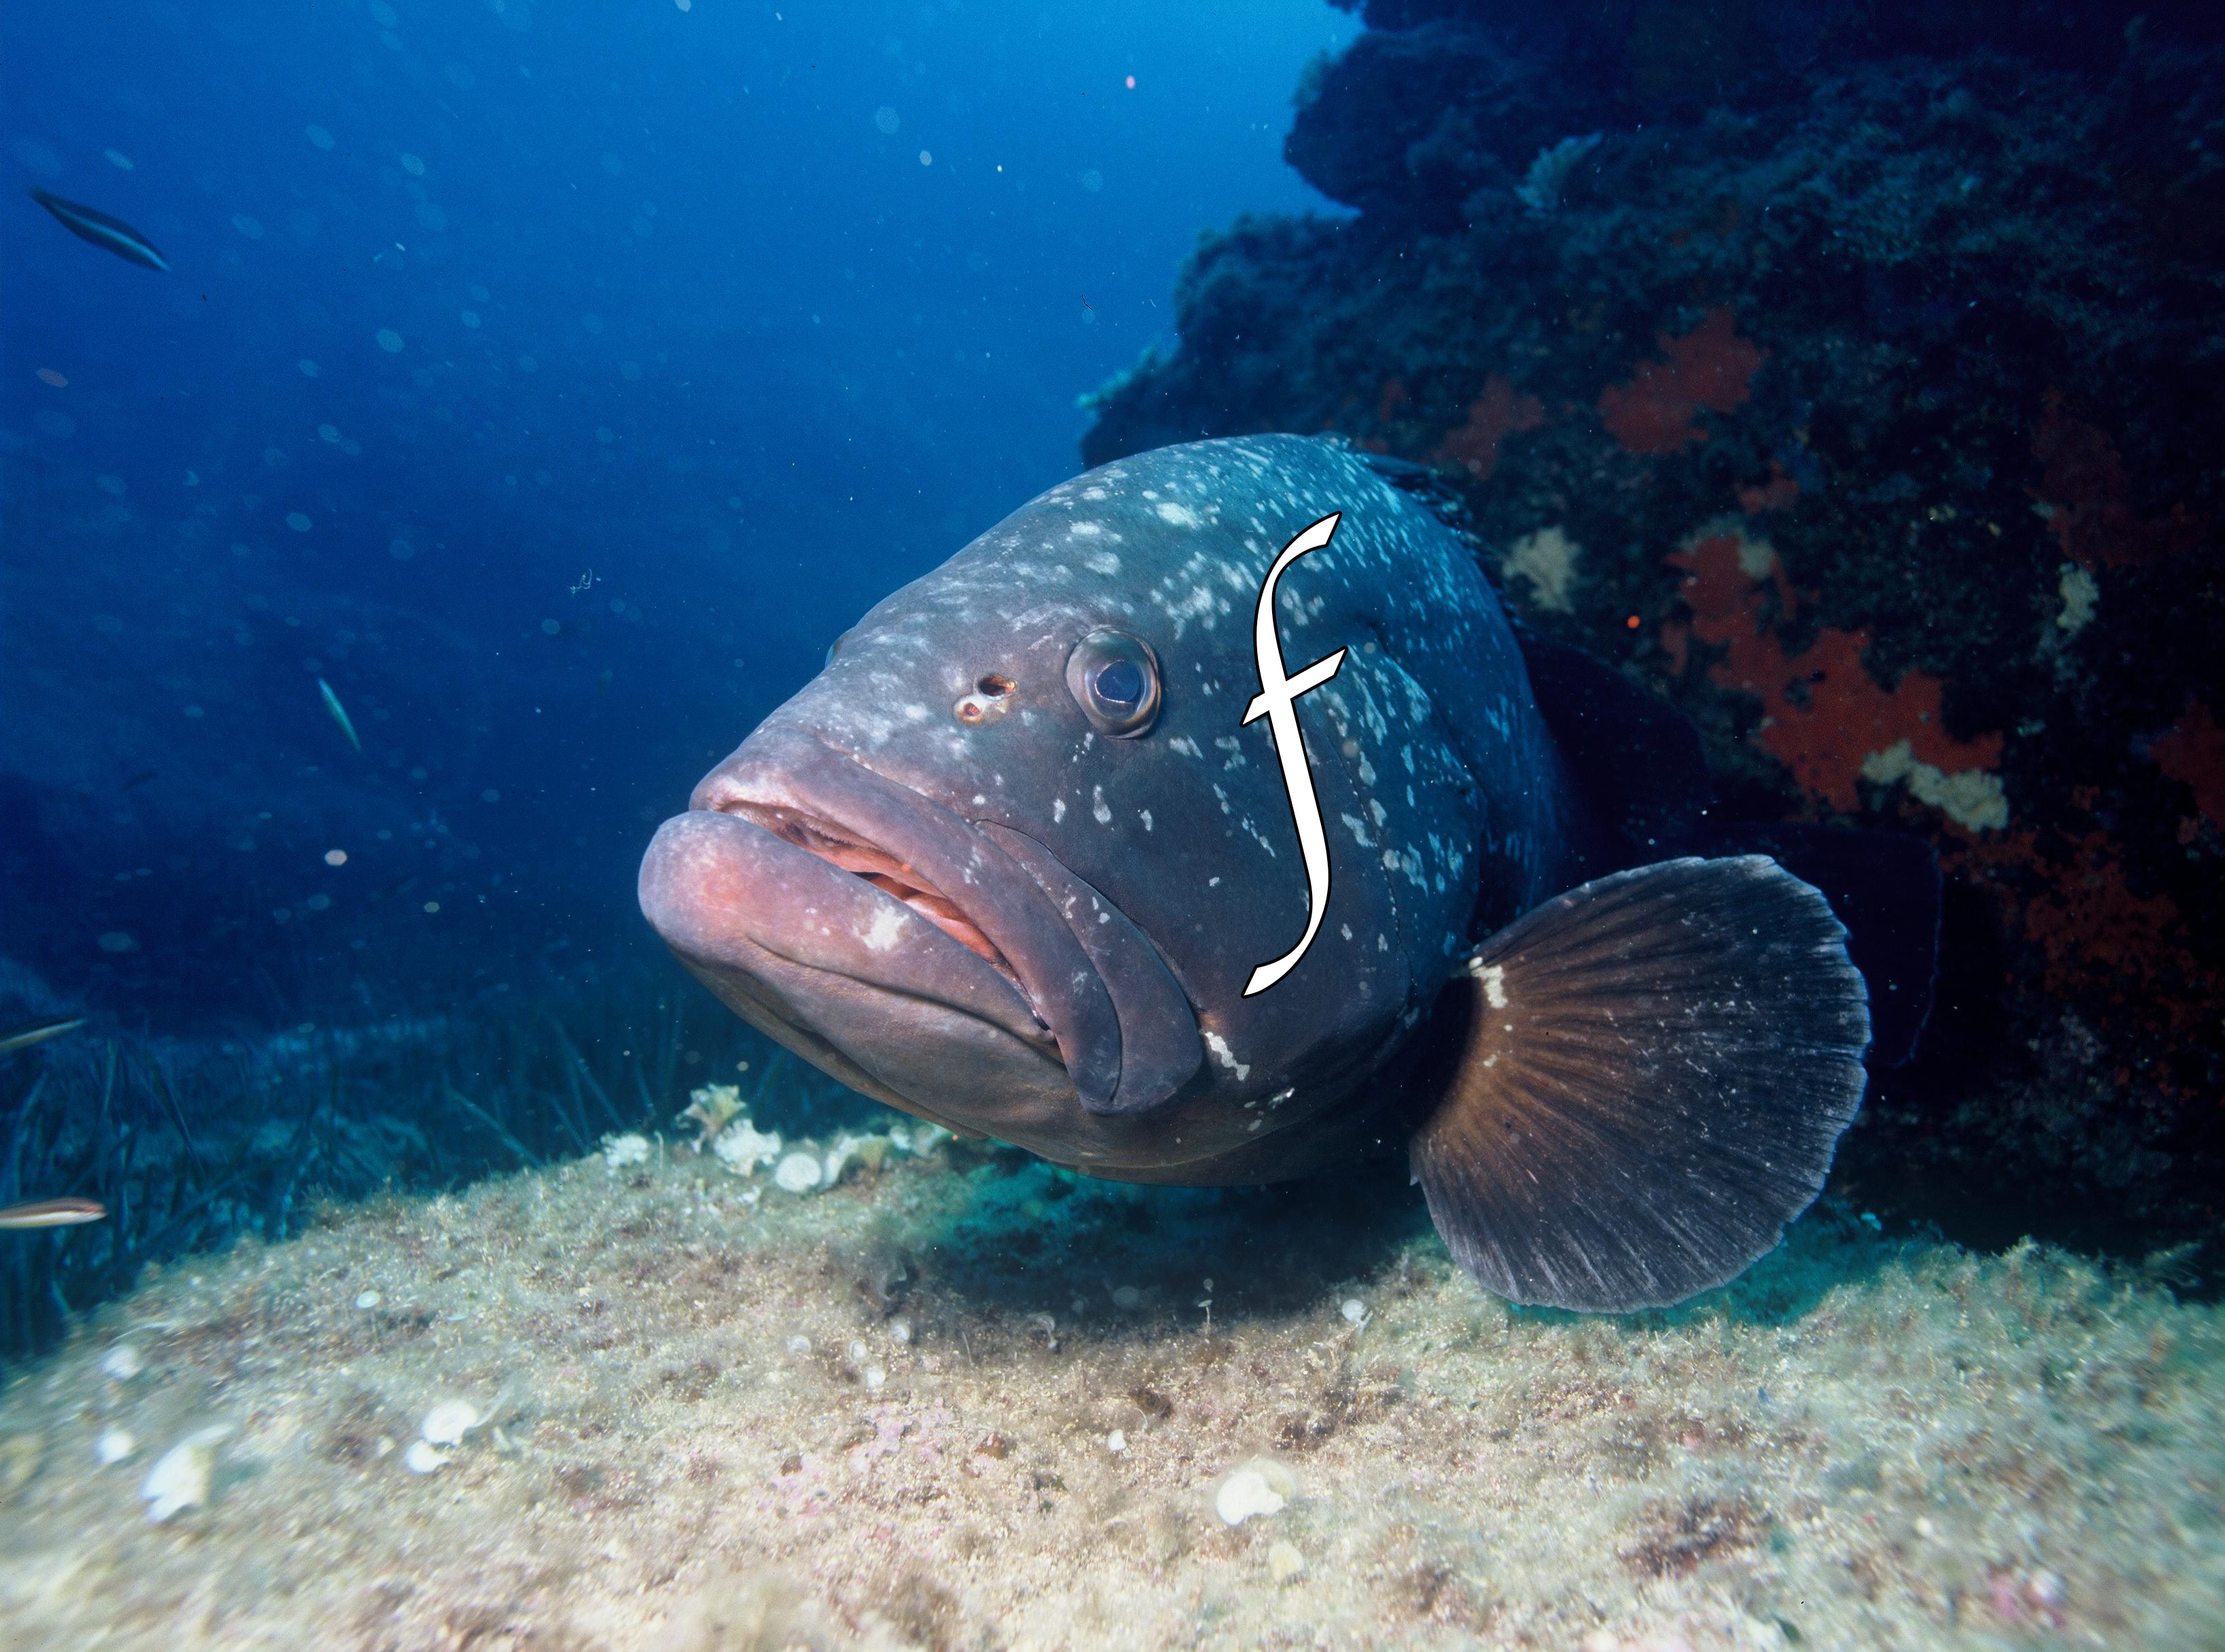
\includegraphics[width=0.8\textwidth]{img/FMeromorfa.jpg}
\caption{Una función meromorfa.}
\end{figure}

\begin{example} Vamos a estudiar un polo de orden 2.

Sea la serie
\[ f(z) = \frac{a_{-2}}{(z - z_0)^2} + \frac{a_{-1}}{(z - z_0)} + a_0 + a_1 (z - z_0) + ... \text{ con } a_{-2} \neq 0\]
Entonces $f(z)$ tiene un polo de orden 2 en $z_0$.

\obs Si $a_{-2} = 0$, entonces el orden del polo \underline{sería 1}.

\noindent {\bf Conclusión:} Si tenemos un polo de orden $m$, la serie de Laurent \underline{empieza en el término $a_{-m}$}.
\end{example}

%\section{Teorema de la singularidad evitable de Riemann}

\section{Teorema de los residuos}
\begin{defn}[Residuos]
Sea $z_0$ una singularidad aislada de una función \\
$\appl{f}{B(z_0,r)\setminus\{z_0\}}{\cplex}$ entonces definimos
\[Res(f(z),z_0)=\frac{1}{2πi}\int_{\partial B(z_0, ε)}f(w)\dif w \ \forall \  ε \in (0,r)\]
\end{defn}

Veamos algunas propiedades:
\begin{enumerate}
\item Sea $0<ε_1<ε_2<r$ por el teorema de Cauchy
\[\int_{\partial B(z_0,ε_2)}f(w)\dif w-\int_{\partial B(z_0,ε_1)}f(w)\dif w = 0\]
es decir, da igual el ε que tomemos.

\item Si $z_0$ es una singularidad evitable el $Res(f(z),z_0)=0$ ya que por el Teorema de Cauchy la integral es 0.

\item Si $f$ tiene un polo de orden $m$ en $z_0$ entonces
\[Res(f(z),z_0)=\frac{1}{(m-1)!}\frac{d^{(m-1)}}{\dif z}\left((z-z_0)^mf(z)\right)\]
\begin{proof}
Tomamos la función $g(z)=(z-z_0)^m f(z)$ que tiene singularidad evitable en $z_0$. Entonces tenemos que
\[\frac{1}{2πi}\int_{\partial B(z_0,ε)} f(z)\dif z = \frac{1}{2πi}\int_{\partial B(z_0,ε)} \frac{g(z)}{(z-z_0)^m} \dif z= \frac{1}{(m-1)!}g^{(m-1)}(z_0)\]
\end{proof}

\item Cálculo del residuo de una singularidad esencial:
\[f(z)=\sum_{n=-\infty}^{\infty} a_n(z-z_0)^n \implies  Res(f(z),z_0)=a_{-1}\]

\begin{proof}
\begin{gather*}
Res(f(z),z_0)= \frac{1}{2πi}\int_{\partial B(z_0,ε)}\left( \sum_{n=-\infty}^{\infty} a_n(z-z_0)^n \right)\dif z \eqreason{conv. uniforme} \\
= \frac{1}{2πi}\sum_{n=-\infty}^{\infty} a_n\int_{\partial B(z_0,ε)}(z-z_0)^n \dif z \eqexpl{\AlignFootnote{por el Th Cauchy, la integral es 0 para $n\neq-1$}} \frac{1}{2πi}a_{-1}\int_{\partial B(z_0,ε)}\frac{1}{z-z_0} \dif z \eqreason{def índice} \\
= \frac{a_{-1}}{2\pi i} \cdot Ind_{\partial B(z_0,\epsilon)} \cdot \frac{2\pi i}{0!} \eqreason{$Ind_{\partial B(z_0,\epsilon)}=1$} a_{-1}
\end{gather*}
\end{proof}

\end{enumerate}

\begin{theorem}[Teorema\IS de los residuos]\label{Th:residuos}
Sea Ω simplemente conexo y sea $f$ una función holomorfa en Ω menos en un conjunto de singularidades aisladas $z_j$. Entonces

\[\int_α f(z)\dif z = 2πi\sum_j Res(f(z),z_j)\cind_α(z_j)\]
siendo α cualquier camino cerrado en Ω que no contenga singularidades.
\end{theorem}


\chapter{Algunos teoremas fundamentales de la variable compleja}
\section{Principio del argumento}
\begin{theorem}[Principio\IS del argumento]
Sea $f$ meromorfa en Ω simplemente conexo y sean $z_j$ los ceros de $f$ (contados con multiplicidad) y sean $p_k$ los polos de $f$.

Entonces para cualquier camino cerrado γ en Ω que no contenga ceros ni polos se tiene que
\[\frac{1}{2πi}\int_γ\frac{f'(z)}{f(z)}dz = \sum_j Ind_γ(z_j)-\sum_k Ind_γ(p_k)\]

Si γ es un camino simple, este principio nos da que la integral es igual al número de ceros que encierra γ menos el número de polos que encierra esta misma curva.

Además
\[\frac{1}{2\pi i}\int_γ \frac{f'(z)}{f(z)} dz = Ind_τ(0) \text{, con } τ=f\circ γ\]
\end{theorem}

\begin{proof}
Por el teorema de los residuos tenemos que
\[\frac{1}{2πi}\int_γ \frac{f'(z)}{f(z)}dz = 2πi\sum_{w \text{ singularidad de } f'/f} Res\left(\frac{f'}{f} \ : \ w\right)Ind_γ(w)\]

Además si $f$ tiene un cero en $\hat{z}$ de orden $n$ tenemos que $f(z)=(z-\hat{z})^ng(z)$ con $g(\hat{z})\neq 0$ y $g$ una función holomorfa cerca de $\hat{z}$

Así, podemos escribir
\[\frac{f'(z)}{f(z)} = \frac{n(z-\hat{z})^{n-1}g(z)+(z-\hat{z})^{n} g'(z)}{(z-\hat{z})^n g(z)} = \frac{n}{z-\hat{z}}+\frac{g'(z)}{g(z)}\]

y por lo tanto
\[Res\left( \frac{f'}{f}\ : \ \hat{z}\right) = \frac{n}{2πi}\int_{\partial B(\hat{z},ε)}\frac{dz}{z-\hat{z}} + \frac{1}{2πi}\int_{\partial B(\hat{z},ε)}\frac{g'(z)}{g(z)}\]
donde la segunda integral es 0 por tratarse de una función holomorfa integrada sobre un camino cerrado.

Si $f$ tiene un polo $p$ de orden $m$ entonces
\[f(z)=\frac{1}{(z-p)^m}g(z)\]
con $g(p)\neq 0$ y $g$ una función holomorfa cerca de $p$.

Por tanto podemos escribir:
\[\frac{f'(z)}{f(z)} = \frac{-m}{z-p}+\frac{g'(z)}{g(z)} \implies Res\left( \frac{f'}{f} \ : \ p \right)=-m\]

\end{proof}

\section{Teorema de Rouché}
\begin{theorem}[Teorema\IS de Rouché]
Sean $f,g$ funciones meromorfas en Ω, siendo este un dominio simplemente conexo, y sea γ un camino cerrado simple en $\Omega$.

Si $f$ y $g$ no tienen polos en γ y además
\[|f(z)-g(z)| < |f(z)|+|g(z)| \ \ \forall z \in γ\]
entonces la diferencia entre el número de ceros y de polos de $f$ encerrados por γ es igual a la diferencia entre el número de ceros y de polos de $g$ encerrados por esta misma curva.

\obs Estamos contando los ceros con su multiplicidad.
\end{theorem}
\begin{proof}

Caso a: Si $g(z)=0$ para algún $z \in γ \implies |f(z)|<|f(z)| \Rightarrow\Leftarrow$

Caso b: Si $f(z)=0$ para algún $z \in γ \implies |g(z)|<|g(z)| \Rightarrow\Leftarrow$

$\therefore$ f y g no tienen ceros en $\gamma$.

Caso c: Si $f$ y $g$ no tienen ceros en γ tenemos:
\[\left| \frac{f(z)}{g(z)}-1\right| < \frac{|f(z)|}{|g(z)|}+1 \text{, para } z \in \gamma\]
Si $\frac{f(z)}{g(z)}=λ\in (-\infty, 0]$ tenemos que $1-λ<λ+1 \iff 0 < \lambda \Rightarrow\Leftarrow$

Entonces $f/g$ es holomorfa en un entorno, $\Lambda$ de γ y, además, omite los valores $\{x \in \real \tq x=0\}$. Por tanto
\[\appl{\log\frac{f}{g}}{\Lambda}{\cplex \setminus \{0\}}\]
\[\left( \log \frac{f}{g}\right) (z) = \log \left|\frac{f(z)}{g(z)}\right| + i Arg \left(\frac{f(z)}{g(z)}\right)\]

Así
\[\left( \log \frac{f}{g}\right)'(z)=\frac{(f/g)'(z)}{(f/g)(z)}=\frac{g(z)}{f(z)}\left[ \frac{f'(z)g(z)-f(z)g'(z)}{g(z)^2} \right] = \frac{f'(z)}{f(z)}-\frac{g'(z)}{g(z)}\]

Por tanto,
\[0 = \frac{1}{2πi}\int_γ \left( \log \frac{f}{g}\right)'dz = \frac{1}{wπi}\int_γ \frac{f'(z)}{f(z)}dz - \frac{1}{2πi}\int_γ \frac{g(z)''}{g(z)}dz =\]
\[=\text{nº de ceros de f - nº de polos de f - (nº de ceros de g - nº de polos de g)}\]
\end{proof}

Veamos algunos ejemplos de la utilidad de este teorema
\begin{example}
Este resultado puede emplearse para demostrar el Teorema Fundamental del Álgebra.

Sea $p(z)=\sum\limits_{i=0}^{n} a_iz^i$ con $a_n\neq 0$ tenemos que $p$ tiene $n$ raíces contadas con su multiplicidad.

\[|p(z)-a_nz^n| = |a_0+a_1z+...+a_{n-1}z^{n-1}| = |a_nz^n|\left| \frac{a_0}{a_nz^n}+ \frac{a_1z}{a_nz^n}+...+ \frac{a_{n-1}z^{n-1}}{a_nz^n}\right|\]
puesto que el segundo factor será menor que 1 para $|z|\geq R$ con $R$ suficientemente grande, tenemos que
\[|p(z)-a_nz^n|  < |a_nz^n|\]
para $|z|=R$ con $R$ grande.

Aplicando el teorema de Rouché tenemos que:
\[\text{nº de ceros de p(z) en} |z|<R = \text{nº de ceros de } a_nz^n \text{ en} |z| < R \]

\end{example}

\begin{example}
\textbf{¿Cuántas raíces de $p(z)=z^4-6z+3$ están en 1<|z|<2?}

Escribimos
\[|p(z)-z^4| = |-6z+3|\leq 6|z|+3 \overbrace{=}^{|z|=2} 15 < 16 \overbrace{=}^{|z|=2}|z|^4 \]
Por tanto, aplicando el teorema de Rouché, tenemos que
\[\text{nº de ceros de p(z) = nº de ceros de } z^4 \text{ en |z|<2}\]

Por otro lado
\[|p(z)+6z|=|z^4+3|\leq |z^4|+3 \overbrace{=}^{|z|=1} 4 < 6\overbrace{=}^{|z|=1}|-6z|\]
y aplicando nuevamente el teorema de Roché vemos que
\[\text{nº de ceros de p(z) en |z|<1= nº de ceros de -6z en |z|<1}\]
\end{example}

\begin{example}
\textbf{Demostrar que $z=λ-e^{-z}$ con λ>1 tiene una única raíz y además esta es real}

Sea $f(z)=z-λ+e^{-z}$
\[f(z)=0 \iff z-λ+e^{-z} = 0 \iff \bar{z}-λ+e^{-\bar{z}}=0 \iff f(\bar{z})=0\]

Es decir, hemos visto que en caso de haber una raíz compleja entonces su conjugado también sería raíz y por tanto tendríamos dos raíces. Si ahora demostramos que la raíz es única tendremos directamente que esta no puede ser compleja.

Ahora vamos a intentar aplicar el Teorema de Rouché. Para ello debemos acotar primero en los puntos con parte real positiva y luego aquellos con parte real nula.

\[|f(z)-(z-λ)|=|e^{-z}|=e^{-Re(z)} \leq 1\]

Sea $R>λ$ vamos a estudiar los puntos $z$ tales que $|z|=R$, Re(z)$\geq 0$.

\[|z-λ|\geq |z|-λ = R - λ > 1 \implies |f(z)-(z-λ)| < |z-λ| \text{ para |z|=R>λ+1}\]

Si ahora tenemos Re(z)=0 y |Im(z)|$\leq R$ tenemos la desigualdad:
\[|z-λ| = \sqrt{|z|^2+λ^2}\geq λ > 1 \text{ (por hipótesis)} \geq |f(z)-(z-λ)|\]

Es decir, ya tenemos que
\[|f(z)-(z-λ)|<|z-λ|<|z|+|λ|\]
por lo que podemos aplicar el teorema de Rouché que nos dice que:
\[\text{ nº ceros de  f - nº polos de f = nº ceros de (z-λ) - nº polos de (z-λ)}\]
y puesto que ambas funciones no encierran ningún polo tenemos que su número de ceros es igual. Como sabemos que $z-λ$ tiene un único cero, concluimos que nuestra función $f(z)$ también tiene un único cero.
\end{example}

\section{Aplicaciones al cálculo de integrales}
Veamos las técnicas a usar para resolver cierto tipo de integrales:
\begin{enumerate}
\item[a)] \textbf{Integrales de la forma}
\[\int_0^{2π}F(\cos \theta, \sin \theta) d \theta\]

Si $z=e^{i\theta}$ entonces
\[\left\{ \begin{aligned}z=\cos(\theta)+i\sin(\theta)\\
\frac{1}{z}=\cos(\theta)-i\sin(\theta) \end{aligned} \right. \implies \left\{\begin{aligned} \cos(\theta)=\frac{z+1/z}{2}\\ \sin(\theta)=\frac{z-1/z}{2i} \end{aligned} \right.\]

Con esto podemos hacer un cambio de variables en la integral dada obteniendo:
\[\int_0^{2π}F(\cos \theta, \sin \theta) d \theta = \int_{|z|=1} F\left( \frac{z+1/z}{2}, \frac{z-1/z}{2i}  \right)\frac{1}{iz}dz = 2πi\sum_{\text{ z singularidad}} Res(f;z)\]
La última igualdad, evidentemente, se deriva del teorema de los residuos

\begin{example}
Tomemos como ejemplo la integral:
\[\int_0^{2π} \frac{\sin^2 \theta}{2+\cos \theta}d\theta = ... = \int_{|z|=1}\frac{(z^2-1)^2i}{2z^2(z^2+4z+1)}dz\]

Aplicamos ahora el teorema de residuos. Para ello miramos primero dónde presenta singularidades esta función. En este caso, las singularidades de la función son los puntos $z_0=0$, $z_1=-2+\sqrt{3}$ y $z_2=-2-\sqrt{3}$.

Puesto que ninguna está en la curva $|z|=1$ vamos por buen camino, ya que el teorema de los Residuos exige que así sea. Aplicando el teorema y obtenemos:
\[\int_{|z|=1}\frac{(z^2-1)^2i}{2z^2(z^2+4z+1)}dz = 2πi\left(Res(f,0)+Res(f,-2+\sqrt{3})+Res(f,-2-\sqrt{3})\right)\]

Calculamos ahora los residuos.

\[z_0=0 \to \lim_{z \to 0} f(z) = \infty \to \lim_{z \to 0} zf(z) = \infty \to \lim_{z \to 0} z^2f(z)=\frac{1}{2}\]
Por tanto sabemos que $z_0$ es un polo de orden 2 por lo que su residuo
\[Res(f,z_0)=\lim_{z \to z_0}(z^2f(z))' = \lim_{z \to z_0}2zf(z)+z^2f'(z) = ... = -2i\]

Por otro lado podemos ver que $z_1$ es un polo de orden 1 pues
\[\lim_{z \to z_1} (z-z_1)f(z) \neq \infty\]
Y su residuo es
\[Res(f,z_1)=\lim_{z \to z_1}(zf(z)\right)' = \lim_{z \to z_1} f(z)+zf'(z) = ... = \sqrt{3}i\]

Por último, vemos que $z_2$ es un polo de orden 1 pero, al no encontrarse dentro de la circunferencia unidad, no debemos tenerlo en cuenta. Así nos queda:

Así, la integral que queremos calcular vale:
\[\int_0^{2π} \frac{\sin^2 \theta}{2+\cos \theta}d\theta = -2i + \sqrt{2}i\]
\end{example}

\item[b)] \textbf{Integrales impropias}

Se trata de integrales de la forma:
\[\int_{-\infty}^{\infty} f(x)dx = \lim_{N \to \infty}\int_{-N}^{\infty}f(x)dx + \lim_{M \to \infty} \int_{-\infty}^{M} f(x)dx\]

Hasta ahora hacíamos el cálculo de estas integrales sin preocuparnos de las velocidades a las que $N$ y $M$ tienen a infinito. Ahora ``si que nos vamos a preocupar'' pues vamos a considerar estas integrales cuando $N$ y $M$ convergen a infinito a la misma velocidad. Al resultado lo llamaremos \concept{Valor principal de Cauchy} y escribimos:
\[V.P. \ \int_{-\infty}^{\infty} f(x)dx = \lim_{N \to \infty}\int_{-N}^N f(x)dx\]

Dentro de estas integrales debemos distinguir diferentes tipos:
\begin{enumerate}
\item[(1)] Sea $f$ holomorfa en Ω$\supset \bar{H}=\{z \tq Im(z)>0\}$ salvo en un número finito de singularidades no reales.

Si $|z|^2f(z)$ está acotado para $|z|$ grande con $Im(z)\geq 0$ entonces
\[\int_{-\infty}^{\infty}f(x)dx = 2πi \sum_{\text{ w singularidad de f}}Res(f,w)\]
y para α > 0 se cumple que:
\[\int_{-\infty}^{\infty} f(x)e^{iαx}dx = 2πi \sum_{\text{w singularidad de f}}Res(f(z)e^{iαz},w)\]
y esta nos permite calcular
\[\int_{-\infty}^{\infty} f(x)\cos(x)dx \text{ y } \int_{-\infty}^{\infty}f(x)\sin(x)\]

\begin{example}
Supongamos que queremos calcular la integral:
\[\int_{-\infty}^{\infty} \frac{x^2-x+2}{(x^2+1)(x^2+4)}dx\]

En este caso tenemos que
\[\lim_{z \to \infty} |z^2||f(z)|=1\]
por lo que está acotado y podremos aplicar el resultado anterior. Por otro lado, puesto que está acotada sabemos que existen dos constantes $C_1, C_2$ tales que $|z^2||f(z)|\leq C_1 \ \forall |z|  \geq C_2$.

Gracias al resultado que estamos estudiando sabemos que la integral impropia converge. La forma de comprobarlo consiste en calcular la integral en $[0,\infty)$ y en $(-\infty, 0]$ y ver que ambas integrales existen. Vamos a ello
\[\int_0^t |f(x)|dx = \int_0^{C_2}|f(x)|dx + \int_{C_2}^t |f(x)|dx \leq K+C_1\int_{C_2}^t \frac{1}{x^2}=K+\frac{C_1}{C_2}-\frac{C_1}{t}\]

Ahora sólo tenemos que ver qué pasa cuando $t \to \infty$. Es inmediato ver que en este caso la integral está acotada por $K+\frac{C_1}{C_2}$.

Hasta aquí hemos comprobado la convergencia no de la función $f(x)$ sino de su valor absoluto. Para poder extender esta convergencia a la función $f(x)$ debemos basarnos en el siguiente truco:

Considero la función
\[G(t)=\int_0^t \left( |f(x)|-f(x)\right)dx\]
vemos que es creciente y acotada superiormente. Puesto que sabemos que $\left( |f(x)|-f(x)\right) \leq 2|f(z)|$ podemos aplicar el mismo truco que hicimos para comprobar la convergencia de $|f(z)|$ llegando a que esta función $G(t)$ está acotada.

Ahora sólo debemos observar que
\[\int_0^tf(x)dx = \int_0^t \left( |f(x)|-(|f(x)-f(x))\right)dx = \lim_{t \to \infty} (F(t)-G(t))\]
con lo que ya tenemos que esta integral es finita.

\textcolor{red}{Mavi: No es importante porque creo que no os vamos a preguntar la convergencia...}

Un cálculo similar podemos hacer para demostrar que existe
\[\lim_{t \to \infty} \int_{-t}^0 f(x)dx\]
con lo que queda claro que la integral que queremos estudiar converge.

Vamos a continuar ahora con el ejemplo. Para ello debemos determinar la región Ω que se encontrará en la parte positiva del eje $OY$ (ya que queríamos que la parte imaginaria fuese positiva). Por comodidad la consideraremos un semicírculo de radio $R$ donde $R$ será suficientemente grande como para contener todas las singularidades de la función.

Las singularidades de la función son $\pm i$ y $\pm 3i$ de modo que basta con tomar $R>3$. Por último también necesitamos que
\[|f(z)| \leq \frac{C_1}{|z|^2} \ \forall |z| \geq R\]
es decir, queremos que la cota que establecimos se cumpla a partir de la frontera\footnote{La cota era válida cuando el módulo de $z$ fuera grande de modo que no podemos pedir que se cumpla en la región interior.}

Aplicamos ahora le teorema de los residuos que nos dice que:
\[\int_{\partial Ω_R} f(z)dz = 2πi\sum_{\text{w singularidad de f}} Res(f,w) = \frac{-1}{16}(1+i)+\frac{1}{48}(3-7i)\]

La integral sobre la frontera se puede escribir como la integral sobre la recta horizontal más la integral sobre la semicircunferencia. Si conseguimos comprobar que cuando $R\to \infty$ esta última integral tiende a 0, tenemos que la integral de la frontera, que sabemos calcular por el teorema de los residuos, será igual a la integral sobre la región horizontal cuando $R \to \infty$. Es decir, nos quedaría que la integral que buscamos coincide con la que hemos calculado en el párrafo anterior.

Veamos si ocurre esto:
\[\left|\int_{\text{arco}}d(x)dz = \right| \left| \int_0^π f(Re^{i\theta})iRe^{i\theta}d\theta\right| \leq \int_0^π |f(Re^{i\theta})|Rd\theta  \leq \int_0^π \frac{C_1}{R^2}Rd\theta = \frac{C_1}{R}π\]
y vemos que, efectivamente, esta integral tiende a $0$ cuando $R$ tiende a infinito.
\end{example}

Veamos otro ejemplo más directo (sin incluir tantas demostraciones teóricas)
\begin{example}
Queremos calcular la siguiente integral
\[\int_0^{\infty}\frac{\cos(αx)}{x^2+β^2} dx \ \ α,β \in \real \ \ α \geq 0, \ β > 0\]

Puesto que esta función es par tenemos que
\[\int_0^{\infty}\frac{\cos(αx)}{x^2+β^2}dx = \frac{1}{2}\int_{-\infty}^{\infty}\frac{\cos(αx)}{x^2+β^2}dx\]

Sea $f(z)=1/(z^2+β^2)$ y sea $g(z)=f(z)e^{iα}$ y podemos ver que la integral que queremos calcular es la parte real de $g(z)$.

Tenemos que $|z²||f(z)| \to 1$ cuando $z \to \infty$. Por otro lado tenemos que:
\[|z^2||g(z)| = |z^2||f(z)|e^{iα}| = |z^2||f(z)|e^{-α Im(z)} \leq |z^2||f(z)| =1\]
por tanto, podemos aplicar el teorema de los residuos sobre la función $g(z)$.

Aplicando el teorema nos queda:
\[\int_{-\infty}^{\infty} \frac{e^{iα}}{z^2+β^2} dz = ... = \frac{π}{β}e^{-αβ}\]

puesto que la integral de un número complejo es la integral de la parte real más $i$ veces la integral de la parte imaginaria tenemos que la integral que queríamos calcular coincide con la parte real del resultado que hemos obtenido. Por tanto:
\[\int_0^{\infty}\frac{\cos(αx)}{x^2+β^2} dx =\frac{π}{β}e^{-αβ} \]
\end{example}

\begin{example}
Tomemos ahora la integral
\[\int_0^{\infty} \frac{x\sin(αx)}{x^2+β^2} = \frac{1}{2}\int_{-\infty}^{\infty}  \frac{x\sin(αx)}{x^2+β^2}\]

Podemos ver que en este caso la función no cumple que $|z|^2|f(z)|$ esté acotado cuando $z \to \infty$. No obstante, si que está acotada si multiplicamos por $|z|$.

La función $f$ que estamos integrando se corresponde con la parte imaginaria de
\[g(z)=f(z)e^{iαz}=\frac{z}{z^2+β^2}e^{iαz}\]

Además existen dos contantes $C_1, C_2 > 0$ tales que
\[|g(z)|=|f(z)||e^{iαz}|=|f(z)|e^{-αIm(z)}\leq \frac{C_1}{|z|}e^{-αIm(z)}\]
para $|z|\geq C_1$, pues $|z||f(z)|\to 1$.

Integramos ahora $g(z)$ en $\partial Ω_R$, siendo $Ω_R$ el semicírculo superior de la circunferencia de radio $R$ centrada en el origen, siendo $R$ suficientemente grande para contener el punto $iβ$.

En estas condiciones tenemos
\[\int_{\partial Ω_R} g(z)dz = 2πiRes(g, βi) = \int_{-R}^{R}f(z)e^{iαz}+\int_{\text{semicírculo}}g(z)dz\]

Pero podemos acotar la segunda integral como:
\[\left| \int_{\text{semicírculo}}g(z)dz \right| = \left| \int_0^π f(Re^{i\theta})e^{iαRe^{i\theta}}iRe^{i\theta}d\theta \right| \leq \int_0^π |f(Re^{i\theta})Re^{-αR\sin(\theta)} d\theta \leq\]

\[\leq C_1 \int_0^π \frac{1}{R}Re^{-R \sin(\theta)}d\theta = C_1 \int_0^π e^{-R \sin(\theta)}d\theta\]

y por el lema de Jordan\footnote{La demostración de este lema se deja como ejercicio para el lector por ser sencilla y de escasa importancia} tenemos que la última integral es menor que $π/R$.

Así, la integral del semicírculo tiende a 0 cuando $R \to \infty$ de modo que, en el límite tendremos:
\[\lim_{R \to \infty} \int_{-R}^{R}\frac{z}{z^2+β^2}e^{iαx} dx = 2πi\cdot Res(\frac{z}{z^2+β^2}e^{iαx}, βi) =\footnote{puesto que βi es un polo simple} 2π i e^{-αβ/2}\]

Puesto que la función que queríamos integral es realmente la parte imaginaria de la función que hemos integrado, debemos tomar la parte imaginaria del resultado obtenido. Es decir
\[\int_0^{\infty} \frac{x\sin(αx)}{x^2+β^2} = πe^{-αβ/2}\]

\end{example}
\newpage
\item[(2)] Sea $f$ holomorfa en Ω $\supset \bar{H}$ salvo un número finito de singularidades y supongamos que tiene singularidades en $\real$ que son polos simples.

Si $|z|^2|f(z)|$ está acotado para $|z|$ grande y $Im(z)\geq 0$ entonces tenemos la siguiente fórmula:
\[V.P. \int_{-\infty}^{\infty}f(x)dx=2πi \left[ \sum_{\text{ w sing de f Im w}\geq 0} Res(f,w)+\frac{1}{2}\sum_{\text{w sing de f Imw=0}}Res(f,w)\right]\]

Veamos algunos ejemplos de cómo aplicar estos resultados.
\begin{example}
Supongamos que tenemos la siguiente integral que queremos resolver
\[\int_0^{\infty} \frac{\sin^2(x)}{x^2}dx = \frac{1}{2}\int_0^{\infty}\frac{1-\cos(2x)}{x^2}=\int_{-\infty}^{\infty} \frac{1-\cos(2x)}{4x^2}dx\]

Sea
\[f(z)=\frac{1-e^{2zi}}{4z^2}\]
tenemos que $|z^2||f(z)|=\frac{1}{4}|1-e^{2zi}| \leq \frac{1}{4}(1+e^{-im(2z)})$ de modo que estamos en las condiciones del resultado que estamos estudiando.\\

Ahora vamos a integrar en el semianillo superior de radios $R$ y $r$ para después hacer tender estos radios a infinito y 0 respectivamente.\\

Tomamos $R$ suficientemente grande para que $|z^2||f(z)| \leq C_1$ para $|z|\geq R, \ Im(z)\geq 0$. Si tenemos alguna singularidad con parte imaginaria positiva tomaremos $R$ grande y $r$ pequeño para que la singularidad se contenga en nuestro $Ω_{R,r}$\\

Por el teorema de los residuos tenemos:
\[0 = \int_{\partial Ω_{R,r}} f(z)dz = \int_r^R f(x)dx +\int_{\text{curva R}}f(z)dz + \int_{-R}^-r f(x)dx + \int_{\text{curva r}} f(z)dz\]

Por otro lado tenemos
\[\left|\int_{\text{curva R}}f(z)dz \right| \leq \int_{\text{curva R}}|f(z)||dz| \leq \int_{\text{curva R}}\frac{C_1}{|z|^2}|dz| = \frac{C_1}{|z^2|}\int_{\text{curva R}}|dz|=\frac{C_1}{R^2}πR \]
y vemos que tiende a 0 cuando $R \to \infty$\\

Vamos a ver ahora que ocurre con la integrar sobre el arco menor.\\

Como $f$ tiene un polo simple en $z_0$ entonces $f(z)=\frac{Res(f,0)}{z}+h(z)$ con $h(z)$ holomorfa y por tanto acotada en la bola de radio $r_0/2$ centrada en el origen y su integral sobre la curva dada tiende a 0 cuando el radio de la curva se hace muy pequeño.\\

Por tanto nos queda:
\[\int_{\text{curva R}} f(z)dz = \int_{\text{curva R}} \frac{Res(f,0)}{x} = Res(f,0)=\int_{\text{curva R}} \frac{dz}{z}=iπRes(f,0)\]

TO BE CONTINUED...

% la integral da π/2


\end{example}
\end{enumerate}
\end{enumerate}

\section{Teorema de la aplicación abierta}



\chapter{Introducción a la representación (transformación) conforme}

\section{Aplicaciones conformes}
\begin{defn}[Aplicación\IS conforme]
Sea $\appl{f}{Ω}{\cplex}$ una aplicación continua, decimos que es conforme en $z_0$ si y sólo si preserva la magnitud y el sentido de los ángulos entre curvas en $z_0$. Es decir:

Sea una función $f$ decimos que es \textbf{conforme} si dadas dos curvas $γ_1, γ_2$ que pasan por $γ(0)=z_0$ cualesquiera se cumple que:
\[\arg\left( \frac{γ_1'(z_0)}{γ_2'(0)}\right)=\arg\left( \frac{f(γ_1(0))}{f(γ_2(0))}\right)=\arg\left( \frac{f'(z_0)}{f'(z_0)}\frac{γ_1'(z_0)}{γ_2'(0)}\right)\]

Por tanto, podemos ver que si $f$ es holomorfa en $z_0$ y $f'(z_0)\neq 0$ entonces será conforme en $z_0$.
\end{defn}

Veamos algunos ejemplos para entender mejor el concepto de conformidad:

\begin{example}
Tomemos la función $f(z)=e^z$ que es holomorfa y, puesto que su derivada no se anula, es conforme.

Consideremos el eje OY y una recta horizontal como curvas sobre las que estudiar la conformidad. Sus imágenes son un radio y una circunferencia respectivamente que, como era de esperar, forman un ángulo recto.
\end{example}

\begin{example}
Tomemos la función $f(z)=z^2$ que es conforme en todo punto distinto del origen.

Es sencillo ver que el efecto de esta curva sobre una recta que pasa por el origen nos da otra recta que pasa por el origen pero tiene radio doble con respecto al eje OX. Si tomamos ahora otra curva que pasa por el origen su imagen tiene ángulo doble que la inicial.

De forma evidente el ángulo que forman estas curvas no se conserva, pues
\[a-b \neq 2a-2b\]
\end{example}

\section{Enunciado del teorema de representación conforme de Riemann}
\begin{theorem}[Teorema\IS de Riemann]
Si Ω es simplemente conexo en $\cplex$ pero $Ω \neq \cplex$. entonces existe $\appl{\phi}{Ω}{\mathbb{D}}$ con $\mathbb{D}=\{z \tq |z|<1\}$ holomorfa y biyectiva.

Si imponemos una serie de condiciones podemos hacer que esta $\phi$ sea única. Estas condiciones son:
\begin{enumerate}
\item $\phi(z_0)=0$

\item $\phi'(z_0)\in \real$

\item $\phi'(z_0) > 0$
\end{enumerate}
\end{theorem}

Decimos que $Ω_1$ y $Ω_2$ son \concept{dominios conformemente equivalentes} si existe una función holomorfa y biyectiva que va de uno al otro.

\obs Todo dominio $Ω\subset \cplex$ simplemente conexo con $Ω\neq \cplex$ es conformemente equivalente a $\mathbb{D}$

\section{Transformaciones de Möbius}

Sea $\appl{f}{\cplex\setminus \{-d/c\}}{\cplex \setminus \{a/b\}}$ definida por
\[f(z)=\frac{az+b}{cz+d} \text{ con } a,b,c,d\in\cplex \text{ y } cz+d \neq 0\]

También podemos pensar en $\appl{f}{\hat{\cplex}}{\hat{\cplex}}$ con la convención:
\[c\neq 0 \implies f(\infty)=a/c \text{ y } f(-d/c)=\infty\]
\[c=0 \implies f(\infty)=\infty\]

Es decir, que hemos pasado de una función que no estaba definida en todo $\cplex$ a una función que lo está incluso en $\hat{\cplex}$

Además, la derivada de $f$ es:
\[f'(z)=\frac{ad-bc}{(cz+d)^2}\]
para $c \neq 0$ es conforme en $\cplex\setminus \{-d/c\}$ para $c=0$ es conforme en $\cplex$

Podemos realizar una cierta \textbf{clasificación de estas transformaciones} según su efecto sobre la función inicial:
\begin{itemize}
\item Si $f(z)=z+z_0$ tenemos una \textbf{traslación}
\item Si $f(z)=λz$ con $λ \in \real^+$ tenemos una \textbf{dilatación}
\item Si $f(z)=kz$ con $|k|=1$ tenemos una \textbf{rotación}
\item Si $f(z)=\frac{1}{z}$ tenemos una \textbf{inversión}.
\end{itemize}

\obs Toda transformación de Möbius es composición de estas transformaciones básicas

\begin{theorem}
Si $f$ es una transformación de Möbius, entonces $f$ lleva de circunferencias en $\hat{\cplex}$ en circunferencias en $\hat{\cplex}$.
\end{theorem}
\obs Las \concept{circunferencias en $\hat{\cplex}$} vistas en el plano son las circunferencias habituales en $\cplex$ y las rectas, que proceden de aquellas circunferencias que pasan por el polo norte en la esfera de Riemann.

Veamos algunos ejemplos:
\begin{example}
Sea
\[f(z)=\frac{z-1}{z+1}\]
Si tomamos la circunferencia unidad, podemos ver que su imagen es el eje OY.

Para ver esto, tomamos tres puntos por los que pase, en orden, la circunferencia. Estos puntos podrían ser $1,-1,i$ y las imágenes por $f$ de estos puntos son $0, \infty, i$ y si los unimos en orden llegamos a la imagen mencionada.

Veamos ahora cómo se comporta sobre el eje OY. Para ello tomamos otros tres puntos por los que el eje pasa de forma ordenada y estudiamos sus imágenes:
\[(-i,i,\infty) \to (-i,i,1)\]
\end{example}

\begin{defn}[Razón doble]
Sean $z_1,z_2,z_3,z_4$ cuatro puntos en $\cplex$ tal que ninguno es infinito, definimos la \textbf{razón doble} como:
\[[z_1,z_2,z_3,z_4]=\frac{(z_1-z_3)(z_2-z_4)}{(z_1-z_4)(z_2-z_3)}\]
Si $z_i=\infty$ la razón doble se define eliminando de la definición los factores que involucran a $z_i$.\footnote{Razón: si calculáis el límite (como si fuesen reales) cuando $z$ tiende a ese $z_i$, lo que esperaríais es que os quedasen los otros términos. Pensadlo.}
\end{defn}

\textbf{Importante:} Si fijamos $z_1,z_2,z_3$, entonces
\[T(z)=[z,z_1,z_2,z_3,z_4]\]
es la única transformación de Möbius tal que
\begin{align*}
z_2 \to 1\\ z_3 \to 0 \\ z_4 \to \infty
\end{align*}
pues
\[T(z)=\frac{(z-z_3)(z_2-z_4)}{(z-z_4)(z_2-z_3)}\]
cumple la propiedad y además es única.

Si hubiese otra, sea $S$, entonces $S\circ T^{-1}$ sería también una transformación de Möbius que fija tres puntos $(1,0,\infty)$.

Pero la única transformación de Möbius que fija tres puntos es la identidad. La demostración de esta última propiedad se deja como ejercicio para el lector.

\begin{lemma}
Si $f$ es transformación de Möbius se cumple:
\[[z_1,z_2,z_3,z_4]=[f(z_1),f(z_2),f(z_3),f(z_4)]\]
\end{lemma}

\begin{proof}
Con la notación anterior, sabemos que $T(z)$ es la única transformación de Möbius que manda:
\begin{align*}
z_2 \to 1\\ z_3 \to 0 \\ z_4 \to \infty
\end{align*}

Por tanto $T\circ f^{-1}$ manda
\begin{align*}
f(z_2) \to 1\\ f(z_3) \to 0 \\ f(z_4) \to \infty
\end{align*}
lo que implica que
\[T\circ f^{-1}(z)=[f(z_1),f(z_2),f(z_3),f(z_4)] \implies \]
\[\implies [z_1,z_2,z_3,z_4] = T(z)=(T \circ f^{-1})(f(z))=[f(z_1),f(z_2),f(z_3),f(z_4)]\]
\end{proof}

\begin{example}
Consideremos la transformación de Möbius tal que
\begin{align*}
1 \to i\\ 0 \to 1 \\ i \to \infty
\end{align*}

En este caso
\[[f(z),f(1),f(0),f(i)]=[z,1,0,i]\implies [f(z),i,0,1]=[z,1,0,i]\implies \]
\[\implies \frac{f(z)-1}{i-1} = \frac{z(1-i)}{(z-i)} \implies f(z)=\frac{z-i+2iz}{z-i}\]

Con lo que ya tenemos calculada la transformación.
\end{example}

\begin{defn}[Orientación]
Sea $τ$ una circunferencia en $\hat{\cplex}$, una \textbf{orientación} en τ es una tripleta ordenada $(z_1,z_2,z_3)$ con $z_1,z_2,z_3 \in τ$.

\obs Si sólo tomásemos dos puntos no sabríamos en que sentido estamos recorriendo la circunferencia ya que si salgo de uno de ellos, da igual en qué sentido recorra la circunferencia por que llegaré al siguiente. Al dar tres puntos evitamos este problema y sólo queda una posible orientación.
\end{defn}

\begin{prop}[Principio de orientación]
Sea $f$ una transformación de Möbius y $τ_1$ una circunferencia en $\hat{\cplex}$ con orientación $z_1,z_2,z_3$. El lado derecho de $τ_1$ va en el lado derecho de $τ_2=f \circ τ_1$ con orientación $(f(z_1),f(z_2),f(z_3))$
\end{prop}

\begin{example}
Encontrar una aplicación holomorfa biyectiva:

\begin{enumerate}
\item De $\{z \tq |z|=1\}$ en $H=\{z \tq Im(z)>0\}$

Para hacerlo basta con identificar tres puntos, ordenados según la orientación de la circunferencia y enviarlos a tres puntos que también están ordenados en la imagen de la aplicación. Así tenemos:
\begin{align*}
1 \to 0\\ i \to 1 \\ -1 \to \infty
\end{align*}

A partir de esta relación calculamos su razón doble:
\begin{gather*}
T(z)=[z,i,1,-1]=\frac{(z-1)(i+1)}{(z+1)(1-i)}=\frac{(z-1)}{(z+1)}\frac{(1+i)(-1-i)}{(i-1)(-i-1)}=\\
=\frac{z-1}{z+1}\frac{-(1+i)^2}{2}=i\frac{1-z}{1+z}
\end{gather*}

¿Y si ahora quisiéramos una nueva transformación $T'$ tal que $T'(0)=3+2i$. Si queremos reutilizar lo anterior, buscaremos una función $\appl{g}{H}{H}$ con $g(0)=3+2i$ y sólo tendríamos que calcular $T'=g \circ T$.

\[T'(z)=2i\left( \frac{1-z}{1+z}\right)+3\]

\end{enumerate}
\end{example}

\section{Automorfismos del disco}

\section{Aplicaciones conformes entre distintos dominios simplemente conexos en el plano}





%% Apéndices (ejercicios, exámenes)
\appendix

\chapter{Ejercicios}
% -*- root: ../VariableCompleja.tex -*-
%%%%%%%%%%%%%%%%%%%%%%%%%%%%%%%%%%%%%%%%%%%%%%%%%%%%%%%%%%%%%%%%%%%%%%%%
%%%%%%%%%%%%%%%%%%%%%%%%%%%%%%%%%%%%%%%%%%%%%%%%%%%%%%%%%%%%%%%%%%%%%%%%
%%                                                                    %%
%%                            HOJA 1                                  %%
%%                                                                    %%
%%%%%%%%%%%%%%%%%%%%%%%%%%%%%%%%%%%%%%%%%%%%%%%%%%%%%%%%%%%%%%%%%%%%%%%%
%%%%%%%%%%%%%%%%%%%%%%%%%%%%%%%%%%%%%%%%%%%%%%%%%%%%%%%%%%%%%%%%%%%%%%%%

\section{Hoja 1}
%
\begin{problem}[1]
Realice las operaciones indicadas
\ppart
\[\frac{1}{i}+\frac{1}{1+i}\]
\ppart
\[\frac{2}{(1-3i)^2}\]
\ppart
\[(1+i\sqrt{3})^3\]
\ppart
\[(\overline{1-i})^2+\overline{2+i}\]

\solution

\spart
\[\frac{1}{i}+\frac{1}{1+i} = \frac{1+i+i}{i-1} = -\frac{2i}{1-i} = \frac{2i(1+i)}{(1-i)(1+i)} = \frac{2i-2}{1+1}=i-1\]

\spart
\[\frac{2}{(1-3i)^2} = \frac{2}{1-9-6i} = \frac{2}{-8-6i}=\frac{2(-8+6i)}{(-8-6i)(-8+6i)} = \frac{2(-8+6i)}{64+36} = \frac{-4+3i}{25}\]

\newpage
\spart
\[(1+i\sqrt{3})^3\ = 1 +3i\sqrt{3}-3\cdot 3-i3^{\frac{3}{2}} = -8 +i (3\sqrt{3}-3\sqrt{3}) = -8\]

\spart
\[(\overline{1-i})^2+\overline{2+i} = \overline{1-1-2i}+2-i = 2i+2-i=2+i\]
\end{problem}

\begin{problem}[2]
Calcule los valores de
\ppart
\[\sum_{k=1}^{2015}i^k\]
\ppart
\[(1+i)^n+(1-i)^n\]
\ppart
\[\left( \cos \left( \frac{\pi}{12} \right) + i \sin \left( \frac{\pi}{12} \right)\right)^{20}\]
\ppart
\[\left(\frac{1+i}{1-i}\right)^{2014}\]
\solution

\spart
Por tratarse de una sucesión geométrica de razón $i$ sabemos que:
\[\sum_{k=1}^{2015}i^k = \frac{1-i^{2015}}{1-i}=\frac{1-\left((i)^4\right)^{503}i^3}{1-i}=\frac{1+i}{1-i}=\frac{1-1+2i}{2}=i\]

\spart
Primero debemos observar que
\large
\[(1+i) = 2^{\frac{1}{2}}e^{\frac{\pi}{4}i}\]
\normalsize
por tanto
\[ (1+i)^n= 2^{\frac{n}{2}}e^{\frac{\pi}{4}in} = 2^{\frac{n}{2}}\left(\cos\left(\frac{\pi}{4}n\right)+i \sin\left(\frac{\pi}{4}n\right)\right)\]

Teniendo en cuenta esta relación, podemos resolver el ejercicio:
\[(1+i)^n+(1-i)^n = (1+i)^n+\overline{(1+i)^n} = 2 Re((1+i)^n)=2^{\frac{n}{2}+1}\cos\left(\frac{\pi}{4}n\right)\]

\spart
\[\left( \cos \left( \frac{\pi}{12} \right) + i \sin \left( \frac{\pi}{12} \right)\right)^{20}=\left(e^{\frac{\pi}{12}}\right)^{20} = e^{\frac{\pi}{12}\cdot 20} = \cos \left( \frac{\pi\cdot 20}{12} \right) + i \sin \left( \frac{\pi\cdot 20}{12} \right) =\]
\[=\cos \left( \frac{\pi\cdot 5}{3} \right) + i \sin \left( \frac{\pi \cdot 5}{3} \right)\]

\spart
Primero vamos a trabajar con el interior del paréntesis para convertirlo en un número complejo en su expresión habitual, sin fracciones.
\[\frac{1+i}{1-i}=\frac{(1+i)^2}{(1-i)(1+i)} = \frac{1-1+2i}{1+1} = i\]
y puesto que el exponente es par, tenemos que
\[\left(\frac{1+i}{1-i}\right)^{2014}=i^{2014}=-1\]
\end{problem}

\begin{problem}[3]
Sea $z=x+iy \in \cplex$. Demuestre que $|x|+|y|\leq \sqrt{2}|z|$, y que sólo hay igualdad si $|x|=|y|$.

\textbf{Ayuda:} Si $a,b \in \real$, entonces $2ab \leq a^2 + b^2$ (con igualdad sólo si $a=b$)

\solution

\doneby{Pedro}

Si calculamos el módulo de z vemos que
\[|z|=\sqrt{x^2+y^2}\]
Si $|x|=|y|$ fácilmente vemos que
\[|z|=\sqrt{x^2+x^2}=\sqrt{2x^2}=\sqrt{2}|x| \implies \sqrt{2}|z|=2|x|=|x|+|y|\]

Veamos ahora el caso en que no son iguales. En esta ocasión, nos apoyamos en al ayuda del enunciado y vemos que
\[|z|=\sqrt{x^2+y^2} \geq \sqrt{2xy} \iff \sqrt{2}|z| \geq 2\sqrt{xy}\]
%TODO terminar esto

%Sin pérdida de generalidad podemos suponer que $|x| > |y|$ y nos queda:
%\[\sqrt{2}|z| \geq 2 \sqrt{xy} \geq 2\sqrt{y^2} \geq 2|y|\]

\end{problem}

\begin{problem}[4]
Compruebe la identidad
\[|z\bar{w}+1|^2+|z-w|^2 = (1+|z|^2)(1+|w|^2)\]
donde $z,w \in \cplex$

\solution

Llamando a $z=a+bi$ y $w=c+di$ tenemos
\[|(a+bi)(c-di)+1|^2+|a+bi+c-di|^2=|ac-adi+bci+bd+1|^2+|a+bi-c+di|^2 = \]
\[=(ac+bd+1)^2+(bc-ad)^2+(a-c)^2+(b+d)^2 =\]
\[= 1 + a²c²+b²d²+2acbd + 2ac+2bd+b²c²+a²d²-2bcad+a^2+c²-2ac+b²+d²-2bd =\]
\[= 1+a²c²+b²d²+b²c²+a²d²+a²+b²+c²+d² = (1+a²+b²)(1+c²+d^2)\]

\end{problem}

\begin{problem}[5]
Demuestra las siguientes afirmaciones
\ppart
\[\text{Si } |z|=1, \text{ entonces para todos } a,b \in \cplex \text{ con } \bar{b}z+\bar{a} \neq 0\text{ se cumple } \left| \frac{az+b}{\bar{b}z+\bar{a}}\right| = 1\]

\ppart
\[\text{Si } |a| < 1, \text{ entonces } |z| <1 \text{ es equivalente a } \left| \frac{z-a}{1-\bar{a}z}\right|<1\]

\solution

\spart


\spart

\[\left| \frac{z-a}{1-\bar{a}z}\right|<1 \iff |z-a| < |1-\bar{a}z| \iff \underbrace{|z-a|^2}_{(z-a)(\bar{z}-\bar{a})} < \underbrace{|1-\bar{a}z|^2}_{(1-\bar{a}z)(1-a\bar{z})} \]

Por lo que nos queda que debe cumplirse
\[|z|^2-a\bar{z}-\bar{a}z+|a|^2 < 1-\bar{a}z+a\bar{z}+|a|^2|b|^2 \iff |z|^2+|a|^2-2\cdot Re(z\bar{a}) < 1 + |a|^2|z|^2-2\cdot Re(z\bar{a}) \iff\]

\[\iff |z|^2 + |a|^2 < 1 +|a|^2|z|^2 \iff |z|^2(1-|a|^2) < 1 - |a|^2 \iff |z|^2 < 1 \iff |z| < 1\]

\end{problem}

\begin{problem}[6]
Usando la fórmula de A. de Moivre, demuestre que
\ppart
$\sin(3x)=3\sin(x)-4 \sin^3(x)$, para todo $x \in \real$

\ppart
Para todo $n \in \nat$ par, la función $\cos(n \phi)$ es un polinomio de grado $n$ de $\cos(\phi)$.

\solution

\spart
Aquí hay que tener algo de idea feliz, aunque sabiendo que estamos trabajando con complejos, tampoco es demasiado raro de pensar.

Vamos a elevar el complejo $\cos(x)+i \sin(x)$ al cubo de dos formas distintas y a igualar los resultados.

\begin{enumerate}
\item
\[\left( \cos(x)+i \sin (x) \right)^3 = (e^{ix})^3 = e^{3ix} = \left( \cos(3x)+i \sin (3x) \right)\]
\item
\[\left( \cos(x)+i \sin (x) \right)^3 = . . . = \cos^3(x)-3\cos(x)\sin^2(x) + i \left( 3\cos^2(x)\sin(x)-\sin^3(x)\right)\]
\end{enumerate}
Ahora, puesto que deben ser iguales las dos representaciones del cubo calculado, debemos igualar las partes reales y las imaginarias.

En este caso, en cuanto forzamos la igualdad de las partes imaginarias obtenemos la igualdad buscada.
\[3\cos^2(x)\sin(x)-\sin^3(x) = \sin(3x) \iff 3\sin(x) - 3 \sin^3(x) - \sin^3(x)=\sin(3x) \iff\]
\[\iff 3\sin(x) - 4 \sin^3(x)=\sin(3x) \]

\spart
El procedimiento a seguir es prácticamente igual que en el caso anterior. Vamos a calcular $\left(\cos(\phi)+i\sin(\phi)\right)^n$ de dos formas distintas
\begin{enumerate}
\item
\[\left(\cos(\phi)+i\sin(\phi)\right)^n = \cos(n\phi)+i\sin(n\phi)\]
\item
\[\left(\cos(\phi)+i\sin(\phi)\right)^n = \sum_{k=0}^n { n \choose k} \cos(\phi)\left( i \sin (\phi)\right)^{n-k}\]
\end{enumerate}

Atendiendo al sumatorio, vemos que vamos a obtener reales siempre que $k$ sea par. En otro caso tendremos siempre un múltiplo de $i$. La suma de esos múltiplos de $i$ acabará siendo $\sin (n\phi)$.

Aplicando esto llegamos a:
\[\cos(n\phi) = \sum_{0 \leq k \leq n} { n \choose k} \cos^k(\phi)(-1)^{\frac{n-k}{2}}\sin^{n-k}(\phi)\]

pero, si nos fijamos en el seno, tenemos que

\[\sin^{n-k}(\phi) = \left(\sin^2(\phi)\right)^{\frac{n-k}{2}} = \left(1-\cos^2(\phi)\right)^{\frac{n-k}{2}}\]

y aplicando esta relación a la igualdad anterior, obtenemos
\[\cos(n\phi) = \sum_{0 \leq k \leq n} (n,k) \cos^k(\phi)(-1)^{\frac{n-k}{2}}\left(1-\cos^2(\phi)\right)^{\frac{n-k}{2}}\]

que, efectivamente, se trata de un polinomio de grado $n$ de $\cos(\phi)$
\end{problem}

\begin{problem}[7]
Demuestre que
\[\left( \frac{1+i\tan(\phi)}{1-i\tan(\phi)}\right)^n = \frac{1+i\tan(n\cdot\phi)}{1-i\tan(n\cdot\phi)}\]

\solution

Vamos a autoconvencernos de que la igualdad es cierta con $n=2$
\[\left( \frac{1+i\tan(\phi)}{1-i\tan(\phi)}\right)^2 = \frac{(1+i\tan(\phi))^2}{(1-i\tan(\phi))^2} = \frac{1-\tan(\phi)^2+2i\tan(\phi)}{1-\tan(\phi)^2-2i\tan(\phi)} = \] \[ =\frac{\cos(\phi)^2-\sin(\phi)^2+2i\sin(\phi)\cos(\phi)}{\cos(\phi)^2-\sin(\phi)^2-2i\sin(\phi)\cos(\phi)}=\frac{\cos(\phi)^2-\sin(\phi)^2+i\sin(2\phi)}{\cos(\phi)^2-\sin(\phi)^2-i\sin(2\phi)}\]
Ahora dividimos entre $\cos(\phi)^2-\sin(\phi)^2$ y, sabiendo que
\[\tan(2 \phi)=\frac{2\sin(\phi)\cos(\phi)}{\cos(\phi)^2-\sin(\phi)^2}\]
tenemos que
\[\frac{\cos(\phi)^2-\sin(\phi)^2+i\sin(2\phi)}{\cos(\phi)^2-\sin(\phi)^2-i\sin(2\phi)}=\frac{1+i\tan(2\cdot\phi)}{1-i\tan(2\cdot\phi)}\]

Ahora vamos a aplicar inducción. Suponemos que la igualdad es cierta para $n$ y vamos a ver qué ocurre con $n+1$.
\[\left( \frac{1+i\tan(\phi)}{1-i\tan(\phi)}\right)^{n+1} =  \frac{\left(1+i\tan(n\cdot\phi)\right)\left(1+i\tan(\phi)\right)}{\left(1-i\tan(n\cdot\phi)\right)\left(1-i\tan(\phi)\right)} = \frac{1-\tan(n\phi)\tan(\phi)+i\left(\tan(\phi)+\tan(n\phi)\right)}{1-\tan(n\phi)\tan(\phi)-i\left(\tan(\phi)+\tan(n\phi)\right)} = \]
multiplicando y dividiendo por $\cos(n\phi)\cos(\phi)$ llegamos a
\[=\frac{\cos(n\phi)\cos(\phi)-\sin(n\phi)\sin(\phi)+i\left(\sin(\phi)\cos(n\phi) + \cos(\phi)\sin(n\phi)\right)}{\cos(n\phi)\cos(\phi)-\sin(n\phi)\sin(\phi)-i\left(\sin(\phi)\cos(n\phi) + \cos(\phi)\sin(n\phi)\right)} =\]
\[=\frac{\cos(n\phi)\cos(\phi)-\sin(n\phi)\sin(\phi)+i\left(\sin((n+1)\phi)\right)}{\cos(n\phi)\cos(\phi)-\sin(n\phi)\sin(\phi)-i\left(\sin((n+1)\phi)\right)}\]
Al igual que hicimos en el caso particular de $n=2$, ahora multiplicamos y dividimos por $\cos(n\phi)\cos(\phi)-\sin(n\phi)\sin(\phi)$ y, sabiendo que
\[\tan((n+1)\phi)=\frac{\sin((n+1)\phi)}{\cos((n+1)\phi)}=\frac{\sin(\phi)\cos(n\phi) + \cos(\phi)\sin(n\phi)}{\cos(n\phi)\cos(\phi)-\sin(n\phi)\sin(\phi)}\]
obtenemos directamente el resultado.

\[\frac{\cos(n\phi)\cos(\phi)-\sin(n\phi)\sin(\phi)+i\left(\sin((n+1)\phi)\right)}{\cos(n\phi)\cos(\phi)-\sin(n\phi)\sin(\phi)-i\left(\sin((n+1)\phi)\right)} =  \frac{1+i\tan((n+1)\cdot\phi)}{1-i\tan((n+1)\cdot\phi)}\]
\obs La última igualdad indicada se obtiene calculando $\sen(α+β)$ y $\cos(α+β)$ con las fórmulas habituales, considerando $α=n\phi$ y $β=\phi$

\end{problem}

\begin{problem}[8]
Sin realizar cálculo alguno, razónese que no es posible que alguno de los valores de $\sqrt[1928]{1+i}$ sea $\frac{1-i}{2}$

\solution
Lo más fácil, en este caso, es ver que los módulos no coinciden. Para ello escribimos
\[1+i = 2^{\frac{1}{2}}e^{(\frac{\pi}{4}+2\pi k)i}\]
y al calcular la raíz obtenemos
\[(1+i)^{\frac{1}{1928}} = 2^{\frac{1}{2\cdot 1928}}e^{(\frac{\pi}{4}+2\pi k)\frac{i}{1928}}\]

Llegados a este punto, podemos ver que los módulos no coinciden, pues
\[2^{\frac{1}{1928}}\neq \left|\frac{1-i}{2}\right| = \sqrt{\frac{1}{2}}\]
\end{problem}

\begin{problem}[9]
Demuestre las siguientes afirmaciones
\ppart
Si $z\neq 1$ entonces
\[\sum_{k=0}^n z^k = \frac{1-z^{n+1}}{1-z}\]

\ppart
Si $ω\neq 1$ es una raíz n-ésima de la unidad, entonces
\[\sum_{k=0}^{n-1} ω^k = \sum_{k=1}^n ω^k= 0\]
y
\[\sum_{k=0}^{n-1} k ω^k = \frac{n}{ω-1}\]

\ppart
si $\sin\left(\frac{\phi}{2}\right)$, entonces
\[\sum_{k=0}^n \cos(k\phi) = \frac{1}{2}\left(1+\frac{\sin((n+\frac{1}{2})\phi)}{\sin\left( \frac{\phi}{2}\right)}\right)\]

y

\[\sum_{k=1}^n \sin(k\phi) = \frac{\sin(\frac{n}{2}\phi)\sin(\frac{n+1}{2}\phi)}{\sin(\frac{\phi}{2})}\]

\textbf{Ayuda:} Use el apartado a) con $z=e^{i\phi}$

\solution
\spart
Vamos a demostrarlo por inducción. En este caso, el caso base es trivial, pues sería $n=1$ con lo que tendríamos
\[1+z=\frac{1-z^2}{1-z}=\frac{(1-z)(1+z)}{1-z} = 1+z\]
Ahora suponemos que la fórmula es válida para $n$ y vamos a ver qué ocurre para $n+1$.
\[\sum_{k=0}^{n+1} z^k = \sum_{k=0}^n z^k + z^{n+1} = \frac{1-z^{n+1}}{1-z} + z^{n+1} = \frac{1-z^{n+1}+z^{n+1}-z^{n+2}}{1-z} = \frac{1+z^{n+2}}{1-z}\]
por lo que queda probado que si la ecuación se cumple para $n$ se cumple también para $n+1$ y, puesto que se cumple para 1, podemos concluir que la ecuación es válida.

\spart
Este caso resulta muy sencillo y rápido si nos apoyamos en el anterior y sabemos que $ω^n=1$ y que $ω^{n+1}=ω$ siendo $ω$ una raíz n-ésima de la unidad.

Por el apartado anterior sabemos que
\[\sum_{k=0}^{n+1} z^k = \sum_{k=0}^n z^k + z^{n+1} = \frac{1-ω^{n+1}}{1-ω}-1 = \frac{1-ω}{1-ω}-1 = 0\]

Para la segunda igualdad simplemente tenemos que darnos cuenta de que
\[\sum_{k=0}^{n-1} k ω^{k-1}  = \frac{\partial}{\partial ω} \sum_{k=0}^{n}ω^k = \frac{\partial}{\partial ω} \frac{1-ω^{n+1}}{1-ω} = \frac{(-n-1)(1-ω)+(1-ω)}{(1-ω)^2} = \frac{-n-1+1}{1-ω}\]

y llegamos a
\[\sum_{k=0}^{n-1} k ω^k = \frac{-n}{1-ω}=\frac{n}{ω-1}\]
\spart
%TODO completar "Lo hice" en clase


\end{problem}

\begin{problem}[10]
Calcule todos los valores de
\ppart
\[\left(-\sqrt{2}-i\sqrt{2}\right)^{1/3}\]
\ppart
\[\sqrt{1-i\sqrt{3}}\]
\ppart
\[\sqrt[4]{1-i}\]
\ppart
\[\left(\sqrt{-i}\right)^{1/3}\]

\solution

\spart
\[\left(-\sqrt{2}-i\sqrt{2}\right)^{1/3}=\left(\sqrt{2}(-1-i)\right)^{1/3}=(\sqrt{2})^{1/3}\left(e^{\frac{-3\pi}{4}+2k\pi}\right)^{1/3}=2^{1/3}e^{\frac{-\pi}{4}+\frac{2}{3}k\pi}\]

\spart
\[\sqrt{1-i\sqrt{3}} = \sqrt{4e^{(\pi/3+2k\pi)i}}=2e^{(\pi/6+k\pi)i}\]

\spart
\[\sqrt[4]{1-i} = \sqrt[4]{\sqrt{2}e^{7\pi/4+2k\pi}} = \sqrt[8]{2}e^{(7\pi/16 + k\pi )i}\]

\spart

\[\left(\sqrt{-i}\right)^{1/3} = \left(1e^{(\pi+2k\pi)i}\right)^{1/6} = e^{(\pi/6+k\pi/3)i}\]
\end{problem}

\begin{problem}[11]
En este ejercicio, consideramos sólo el \textit{valor principal de la raíz cuadrada}, definido como
\[\sqrt[(p)]{z}=\sqrt{r}\left(\cos\frac{\phi}{2}+i\sin\frac{\phi}{2}\right)\]
cuando $z=r(\cos\phi+i\sin\phi)$ con $-\pi < \phi < \pi$. Claramente, $\left( \sqrt[(p)]{z} \right)^2=z$
\ppart Demuestra que las soluciones en $\cplex$ de la ecuación $az^2+bz+c=0$, con $a\neq 0$, son
\[z=\frac{-b\pm \sqrt[(p)]{b^2-4ac}}{2a}\]
\ppart
Calcule
\[\sqrt[(p)]{\left(\sqrt[(p)]{i}\right)^5} \text { y } \sqrt[(p)]{1+\sqrt[(p)]{i}}\]
\solution

\spart
Para resolver este apartado basta son sustituir la fórmula que nos dan para la $z$ en la ecuación dada y comprobar que, efectivamente, la ecuación se verifica.

\spart
La raíz principal puede sonar a algo exótico pero consiste, simplemente, en tomar la raíz del número dado y, en lugar de considerar los varios ángulos posibles, tomamos el menor posible (siempre positivo).

A efectos legales esto nos hace ahorrarnos el típico $+2k\pi$. Veamos a modo de ejemplo los radicales que nos pide calcular el enunciado
\[\sqrt[(p)]{\left( \sqrt[(p)]{i}\right)^5} = \sqrt[(p)]{e^{-\frac{3\pi}{4}i}} = e^{-\frac{3\pi}{8}}i\]

\[\sqrt[(p)]{1+\sqrt[(p)]{i}} = \sqrt[(p)]{1+\sqrt[(p)]{i}} = \sqrt[(p)]{1+\sqrt{2}/2+i\sqrt{2}/2} = \sqrt{2+\sqrt{2}}\left( \cos\left(\frac{π}{4}\right)+i\sin\left(\frac{π}{4}\right)\right)\]
\end{problem}

\begin{problem}[12]
Resuelve las siguientes ecuaciones:
\ppart
\[(z+1)^4+i=0\]
\ppart
\[Re(z^2+5)=0\]
\ppart
\[Re(z+5)=Im(z-i)\]
\solution

\spart
Despejando como hemos hecho siempre tenemos que
\[z=\sqrt[4]{-i}-1 = e^{\pi/4+\pi k / 2} -1 \]

\spart
Considerando $z=x+iy$ tenemos que $z^2=x^2-y^2+2xyi$ con lo que llegamos a
\[x^2-y^2 = -5\]
que nos da una hipérbola

\spart
Considerando $z=x+iy$ tenemos
\[Re(z+5)=Im(z-i) \iff x+5=y-1\]
obteniendo como resultado una recta.

\end{problem}

\begin{problem}[13]
\ppart
Demuestra que si $α$ es solución de $z^n=μ$ (con $μ\in\cplex$ fijo), entonces todas las soluciones son $αω_i$ con $i=0,1,...,n-1$ donde $ω_i$ son las raíces n-ésimas de la unidad
\ppart
Encuentre razonadamente las soluciones de $z^6-8=0$
\solution
\doneby{Pedro}

\spart
Es sencillo e ver que los números de la forma $αω_i$ son soluciones, puesto que
\[(αω_1)^n = α^n ω_i^n= μ \cdot 1 = μ\]
Cualquier otra hipotética solución deberá cumplir que al elevarla a $n$ obtengamos μ, por lo que deberá ser $α$ multiplicado por algo que, al elevarlo a $n$ nos de 1. Es decir, no habrá más posibilidades que las indicadas

\spart
Siguiendo lo indicado en el apartado anterior las soluciones serán de la forma:
\[z=\sqrt[6]{8}ω_i \text{ con } i=0,1,2,3,4,5 \text{ y } ω \text{ raíz sexta de la unidad}\]

\end{problem}

\begin{problem}[14]
¿Cuándo son colineales tres puntos $z_1,z_2,z_3$ distintos dos a dos?
\solution
Para verlo hacemos como en bachillerato con los reales: escribimos la recta que pasa por dos de esos puntos y forzamos a que el tercero se contenga en dicha recta.

La recta que pasa por $z_1$ y $z_2$ sería:
\[L=\{z_1+t(z_2-z_1) t \in \real \}\]
Si $z_3 \in L \implies \exists t \tq z_3=z_1 + t(z_2-z_1)$ es decir:
\[t = \frac{z_3-z_1}{z_2-z_1}\in \real\]
para que sea real ese resultado necesitamos que el numerador y el denominador tengan el mismo argumento.

Intuitivamente representa que uniendo $z_3$ con $z_1$ obtenemos la misma recta que uniendo $z_2$ con $z_1$
\end{problem}

\begin{problem}[15]

\ppart
Compruebe que la ecuación
\[Re(az+b) = 0 \text{ con } a,b\in \cplex, \ a \neq 0\]
define una recta en el plano y que, recíprocamente, cada recta viene descrita por una ecuación de este tipo

\ppart
Encuentre los números $a,b$ para que la recta pase por dos puntos dados $z_1, z_2 \in \cplex$

\ppart
Demuestre que las rectas determinadas por las ecuaciones $Re(az+b)=0$ y $Re(cz+d)=0$ respectivamente, son perpendiculares si y sólo si $Re(a\bar{c})=0$

\ppart
Demuestre que la ecuación de una recta que pasa por dos puntos dados $z_1$ y $z_2$ puede escribirse de la forma
\[ \left| \begin{array}{ccc}
z  & \bar{z} & 1 \\
z_1 & \bar{z_1}&  1 \\
z_2 & \bar{z_2} & 1 \end{array} \right| = 0\]

\solution
\doneby{Pedro}

\spart

Siendo cada número complejo $x\in \cplex = x_r+ix_i$, la ecuación que nos dan se traduce en
\[a_rz_r-a_iz_i+b_r=0 \equiv z_i = \frac{a_rz_r+b_r}{a_i}\]
siendo $x_i = y$ y $z_r = x$ obtenemos la ecuación de una recta en el plano.

\spart

Basta con sustituir en la ecuación los valores $z_1=z_{1r}+iz_{1i}$ y $z_2=z_{2r}+iz_{2i}$ y obtenemos un sistema de 4 ecuaciones de 4 incógnitas que podremos resolver.

\textcolor{green}{Plan b como alternativa distinta que me convence más}

Utilizando la ecuación $z_i = \displaystyle\frac{a_rz_r+b_r}{a_i}$ escribimos un sistema de 2 ecuaciones con 3 incógnitas, que tiene sentido que salga un sistema indeterminado con infinitas soluciones (puedo coger como $b∈ℂ$ cualquiera que pertenezca a la recta)

\[
\begin{array}{cc}
Im(z_2) = \frac{a_r Re(z_2) - b_i}{a_i}\\
Im(z_1) = \frac{a_r Re(z_1) - b_i}{a_i}
\end{array}
\]

\spart

Basándonos en el apartado a), podemos ver que las pendientes de esas rectas son, respectivamente, $\frac{a_r}{a_i}$ y $\frac{c_r}{c_i}$.

Para que sean perpendiculares, debemos tener
\[\frac{a_r}{a_i}= - \frac{c_i}{c_r} \implies a_rc_r = -a_ic_i \implies Re\left((a_r+ia_i)(c_r-ic_i)\right) = 0\]

\spart
%TODO por hacer

\end{problem}

\begin{problem}[16]
Describa el conjunto del plano complejo determinado por las siguientes relaciones
\ppart
\[|z-2|-|z+2| > 3\]
\ppart
\[Re(z)+Im(z) < 1\]
\ppart
\[|2z|>|1+z^2|\]

\solution
\doneby{Pedro}

\spart
Si tuviéramos una igualdad, estaríamos hablando de los puntos del plano cuya diferencia de distancias a los puntos $(2,0)$ y $(-2,0)$ es constante. Es decir, tendríamos una hipérbola.

Al tener una desigualdad, estamos cogiendo aquellos puntos situados a la derecha de la hipérbola.

\spart

Esta ecuación representa aquellos puntos del plano que quedan a la izquierda de la recta $y=-x+1$.

\spart



\end{problem}

\begin{problem}[17]
Determine las ecuaciones complejas:
\ppart de la parábola con foco i y directriz $Im(z)=-1$
\ppart de la elipse con focos $\pm 1$ que pasa por $i$
\ppart de la hipérbola con focos $\pm 1$ que pasa por $i+1$

\solution

Este ejercicio es bastante semejante a los apartados b) y c) del ejercicio 1.10

\spart
Recordemos que una parábola se definía a partir del foco y la directriz como el conjunto de puntos del plano que equidistaban de ellos.

Para escribir la ecuación, simplemente aplicamos la definición y vemos a que ecuación nos lleva.

Sea un punto cualquiera $z=x+iy$ su distancia al foco $i$ sería $|z-i|$ mientras que la distancia a la directriz sería $1+Re(z)$

Igualando tenemos la ecuación buscada
\[|z-i|=Re(z)+1\]

\spart
Recordemos que, por definición, la elipse es el conjunto de puntos del plano con suma de distancias a los focos constante.

Conocemos los focos lo que nos lleva a:
\[|z-1|+|z+1|=cte\]

Para determinar la constante nos basamos en que pasa por $i$, lo que nos lleva a concluir que la constante es $2\sqrt{2}$ es decir, nos queda la ecuación
\[|z-1|+|z+1|=2\sqrt{2}\]

\spart
La hipérbola tenía definición similar a la de la elipse salvo que en este caso considerábamos constante la diferencia de distancias a los pocos en lugar de la suma.

De aquí obtenemos que la ecuación buscada será de la forma
\[|z-1|-|z+1|=cte\]
Sabiendo que pasa por el punto $i+1$ podemos calcular la constante
%TODO completar

\end{problem}

\begin{problem}[18]
Esboce el conjunto de puntos $z \in \cplex$ que satisfacen
\ppart \[Re\left( \frac{z}{1+i}\right) = 0\]
\ppart \[|z^2-4z+4| = 4\]
\ppart \[|z^2-2z-1|=1\]

\solution

\spart
Vamos a jugar un poco con el número que nos dan. Siendo $z=x+iy$ tenemos
\[\frac{x+iz}{1+i}\cdot\frac{1-i}{1-i} = \frac{x-y+i(y-x)}{2} \implies Re\left( \frac{z}{1+i}\right) = \frac{x-y}{2}\]

Por tanto, obtenemos la recta $y=x$, la bisectriz del primer cuadrante.

\spart
\[z^2-4z+4| = 4 \iff |z-2|^2 = 4 \]
con lo que tenemos una circunferencia

\spart
Se deja como ejercicio para el lector, que deberá pasar a coordenadas polares con el objetivo de poder esbozar el dibujo pedido.

\textbf{consejo:} Acordarnos de la Lemniscata
\end{problem}

\begin{problem}[19]
\ppart Sea $a \in \cplex$ un número fijo. Encuentre el máximo de $|z^{12}-a|$ cuando $z$ es cualquier número complejo tal que $|z|\leq 1$
\ppart Halle razonadamente el supremo y el ínfimo del siguiente conjunto de números reales
\[\{Re(iz^4+1) \tq |z|<\sqrt{2}\}\]

\solution
\doneby{Pedro}

\spart
Si abordamos el ejercicio como un problema en $\real^2$, lo que tenemos es que nos dan un punto cualquiera del plano y debemos buscar el punto del círculo unidad que más diste de él.

Para ello basta con unir el punto dado con el centro y prolongar el segmento que los une hasta que corte a la circunferencia.

Es decir, dado el punto $a=r\left(\cos(\theta)+i\sin(\theta)\right)$, el punto $b$ del círculo unidad más alejado de $a$ es $b=1\left(\cos(\theta +2π)+i\sin(\theta +2π)\right)$

(Posiblemente habría que tener cuidado si el punto $a$ no pertenece al primer cuadrante)

Para calcular ahora el número $z$ pedido, basta con tomar z=$\sqrt[12]{b}$

\spart
Siendo $z=x+iy$ tenemos
\[Re(iz^4+1)=x^4+y^4-6x^2y^2+1\]

Como aprendimos a hacer en Cálculo I, tenemos que calcular el gradiente de esa función e igualarlo a 0 y posteriormente estudiar el comportamiento de la función en la frontera del conjunto que estamos estudiando.

Vamos con el gradiente
\[\nabla \left(Re(iz^4+1)\right) = \left(4x^3-12xy^2, 4y^3-12x^2y\right)\]
al igualarlo a 0 tenemos que los puntos extremos son: el origen y los puntos que satisfacen a la vez las ecuaciones:
\[x^2-3y^2=0\]
\[y^2-3x^2=0\]
que viene a no decir nada y a dejarnos igualmente restringidos al origen

Para estudiar el comportamiento de la función en la frontera del conjunto estudiado tenemos
\[|z| = \sqrt{2} \implies x^2+y^2 =2 \implies y=\sqrt{2-x^2} \]
sustituyendo en la fórmula estudiada tenemos:
\[x^4+4+x^4-4x^2-12x^2+6x^4 +1 =0\]
derivando y simplificando tenemos
\[32x^3-32x=0 \implies x^2-1=0 \implies x=\pm 1 \implies y = \pm \sqrt{3}\]
Los puntos de máximo y mínimo son $(\pm 1, \pm \sqrt{3})$

\end{problem}

\begin{problem}[20]
Describa geométricamente el conjunto de los puntos $w \in \cplex$ que se escriben en la forma $w=iz^2+1$, para $z=x+iy$ con $x>0, y>0, \ x^2+y^2<1$.

\solution

Operando, tenemos que estamos trabajando con el conjunto de números complejos de la forma:
\[w=i(x^2-y^2)-2xy+1\]


\end{problem}

\begin{problem}[21]
Demuestre que, dados $a,c \in \cplex$, la condición necesaria y suficiente para que exista $z \in \cplex$ que verifique $|z+a|+|z-a|=2|c|$ es que sea $|a|\leq|c|$

\textbf{Ayuda:} Si $λ>0$, el conjunto $ \{z \in \cplex \tq |z+a|+|z-a|=2λ\}$ es una elipse si $λ > |a|$, un segmento si $λ=|a|$ y el conjunto vacío si $λ<|a|$

\solution

Basándonos en la indicación dada es obvio que $|a|\leq|c|$ es condición necesaria y suficiente para que podamos hablar de la solución de la ecuación ya que, en caso contrario, tendríamos el vacío.

Si tenemos $|a|\leq|c|$ el conjunto de puntos solución de la ecuación constituirán una recta o una elipse (según el caso) pero en ambos casos son conjuntos válidos que nos dan solución para la ecuación.
\end{problem}

\begin{problem}[22]
He aquí algunas interpretaciones geométricas de ciertas operaciones con números complejos.

\ppart Si $z=x+iy \in \cplex$ sea $α(z)$ el vector de tres dimensiones $(x,y,0)$. Verifique que para cada $z,w \in \cplex$ se cumple que $α(z)α(w)=Re(z\bar{w})$ y $α(z)\times α(w)=(0,0,Im(\bar{z}w))$

\ppart Si $0,z,w$ son los vértices de un triángulo $T$, compruebe que $Area(T)=\frac{1}{2}|Im(\bar{z}w)|$

\ppart
Si $z_1, z_2,...z_n$ son los vértices de un polígono $P$ que contiene a 0 en su interior, demuestra que $Area(P)=\frac{1}{2}\left|Im\left( \sum_{j=1}^n \bar{z}_jz_{j+1}\right)\right|$, donde se toma $z_{n+1}=z_1$

\solution
\doneby{Pedro}

\spart
\[α(z)α(w)=z_xw_x+z_yw_y\]
Por otro lado
\[Re(zw)=Re\left(z_xw_x+z_yw_y+i(z_xw_y-z_yw_x)\right) = z_xw_x+z_yw_y \]

Si calculamos el producto vectorial que se nos pide, tenemos que
\[α(z)\times α(w) = (0,0,-z_xw_y+z_yw_x)\]
que podemos comprobar que coincide con la parte imaginaria de
\[Im(\bar{z}w) = Im \left( z_xw_x-z_yw_y+i(-z_xw_y+z_yw_x)\right)\]

\spart

Si ya hemos visto que el producto vectorial coincide con la parte imaginaria, es trivial ver que un medio de esa parte imaginaria nos dará el área del triángulo, pues el producto vectorial nos da el área del paralelogramo generado por los dos vectores.

\spart
Con imagen del producto que se nos da (tras multiplicar por 1/2) obtenemos el área del triángulo formado por los dos puntos dados y el origen.

Puesto que el origen se contiene en la figura cuyo área estamos calculando, al hacer esta operación con todos los vértices tenemos el área de la figura.

\end{problem}

\begin{problem}
Demuestre que la condición necesaria y suficiente para que $\{z_1, z_2, z_3\}$ sea el conjunto de los vértices de un triángulo equilátero es que
\[z_1z_2+z_2z_3+z_3z_1=z_1^2+z_2^2+z_3^2\]
\textbf{Ayuda:} Considere el triángulo $\{z_2, z_3,z_1\}$

\solution

\end{problem}


%%%%%%%%%%%%%%%%%%%%%%%%%%%%%%%%%%%%%%%%%%%%%%%%%%%%%%%%%%%%%%%%%%%%%%%%
%%%%%%%%%%%%%%%%%%%%%%%%%%%%%%%%%%%%%%%%%%%%%%%%%%%%%%%%%%%%%%%%%%%%%%%%
%%                                                                    %%
%%                            HOJA 2                                  %%
%%                                                                    %%
%%%%%%%%%%%%%%%%%%%%%%%%%%%%%%%%%%%%%%%%%%%%%%%%%%%%%%%%%%%%%%%%%%%%%%%%
%%%%%%%%%%%%%%%%%%%%%%%%%%%%%%%%%%%%%%%%%%%%%%%%%%%%%%%%%%%%%%%%%%%%%%%%
\newpage
\section{Hoja 2}
\begin{problem}[1]
(\textit{Esfera de Riemann}) Se considera $\widehat{\cplex} = \cplex \cup \{\infty\}$ y se definen los entornos de $\infty$ como aquellos que contienen un conjunto de la forma $\{z \in \cplex \tq |z|>R\}$ para algún $R > 0$

Con estos entornos $z_n \to \infty$ quiere decir que
\[\forall R > 0 \exists N \tq |z_n| > R \ \forall n > N\]

De manera similar se definen $\lim_{z \to b} f(z)= \infty$ y $\lim_{z \to \infty}f(z)=\infty$.

Sean $\mathbb{S}= \{p \in \real^3 : p_1^2+p_2^2+p_3^2\}$ y consideramos la proyección estereográfica:
\[\appl{\pi}{\mathbb{S}}{\widehat{\cplex}}, \pi(p) = \left\{
\begin{array}{lcc}
    \frac{(p_1+ip_2)}{1-p_3} & si & p \neq N = (0,0,1) \\
 \\ \infty & si & p = N
 \end{array} \right.\]

 \ppart
 Compruebe que
 \[\pi^{-1}(z)=\left( \frac{2Re(z)}{|z|^2+1}, \frac{2Im(z)}{|z|^2+1}, \frac{|z|^2-1}{|z|^2+1}\right)\]

 \ppart
 Sea $\rho(z,w)$= distancia (en $\real^3$) entre $\pi^{-1}(z)$ y $\pi^{-1}(w)$ para $z,w \in \widehat{\cplex}$. Entonces:
 \[z_n \to z \text{ en } \widehat{\cplex} \implies \rho(z_n,z) \to 0\]

 \ppart
 Demuestre que
 \[\lim_{n \to \infty}\frac{z^n}{n} = \infty \text{ si } |z| > 1\]

\solution
\doneby{Edu}

\spart

Sea $z=0$ el plano sobre el que haremos la proyección estereográfica.

Sea
\[r=\left\{
\begin{pmatrix}x\\y\\z\end{pmatrix} =  \begin{pmatrix}x_0\\y_0\\0\end{pmatrix} t + (1-t) \begin{pmatrix}0\\0\\1\end{pmatrix} = \begin{pmatrix}x_0t\\y_0t\\1-t\end{pmatrix}
\right\}\]
la recta que pasa por el polo norte y el punto $(x_0,y_0,0)$.

Calculemos la intersección con $\mathbb{S}$:
\begin{gather*}
(x_0t)^2 + (y_0t)^2 + (1-t)^2 = 1 \\
x_0^2 t^2 + y_0^2 t^2 + 1 - 2t + t^2 = 1 \\
x_0^2 t^2 + y_0^2 t^2 - 2t + t^2 = 0 \\
t ( x_0^2 t + y_0^2 t - 2 + t) = 0\\
\end{gather*}

Luego las soluciones son
\begin{center}
$t = 0$ (polo norte) y\\
$x_0^2 t + y_0^2 t - 2 + t = 0 \iff t = \frac{2}{x_0^2 + y_0^2 + 1}$.
\end{center}

Luego
\[\begin{pmatrix}x\\y\\z\end{pmatrix} = \begin{pmatrix} \frac{2x_0}{x_0^2 + y_0^2 + 1} \\ \frac{2 y_0}{x_0^2 + y_0^2 + 1} \\ 1-\frac{2}{x_0^2 + y_0^2 + 1} \end{pmatrix} = \begin{pmatrix} \frac{2x_0}{x_0^2 + y_0^2 + 1} \\ \frac{2 y_0}{x_0^2 + y_0^2 + 1} \\ \frac{x_0^2 + y_0^2 - 1}{x_0^2 + y_0^2 + 1} \end{pmatrix}\]

Tomando $w = x_0+iy_0 \implies |w|^2 = x_0^2+y_0^2$, $Re(w) = x_0$, $Im(w) = y_0$:
\[ \begin{pmatrix}x\\y\\z\end{pmatrix} = \begin{pmatrix} \frac{2Re(w)}{|w|^2 + 1} \\ \frac{2 Im(w)}{|w|^2 + 1} \\ \frac{|w|^2 - 1}{|w|^2 + 1} \end{pmatrix}\]
\qed

\textcolor{blue}{Hecho por Pedro}\\
\spart

Ya sabemos que si una sucesión de complejos converge a un complejo dado es por que tanto la parte real como la imaginaria lo hacen por separado. Así mismo, eso implica directamente que la sucesión de los módulos converge al módulo del límite.

Una vez visto esto es obvio ver que la implicación dada es correcta.

\spart

La forma más sencilla de ver esto es trabajando sobre la inversa de la proyección estereográfica. Puesto que es un homeomorfismo (ya lo estudiamos en Análisis) sabemos que $π^{-1}$ es continua por lo que la imagen límite de una sucesión es el límite de las imágenes.

Nos llevamos por tanto los puntos $z_n=\frac{z^n}{n}$ a la esfera y vemos que van creciendo en módulo. Cuando el módulo tiende a infinito, $π^{-1}$ tiene al $(0,0,1)$

\textcolor{blue}{Explicación guarrísima. Trataré de mejorarla.}

\end{problem}

\begin{problem}[2]
\ppart
Demuestre que, mediante la proyección estereográfica, las circunferencias sobre la esfera se transforman en circunferencias o rectas del plano. ¿Cuáles son las circunferencias sobre la esfera que se transforman en rectas?

\ppart
¿Qué corresponde en la esfera de Riemann a una familia de rectas paralelas del plano?

\ppart
Halle, en la esfera de Riemann, las imágenes de los conjuntos definidos por las siguientes desigualdades:
\begin{enumerate}
\item $Im(z) > 0$
\item $Re(z) < 1$
\item $|z| < 1$
\item $|z| > 2$
\end{enumerate}

\solution

\textcolor{blue}{La profesora escribió algunas cuentas pero no me han parecido muy útiles ni novedosas. Aquí doy la idea del ejercicio.}

\spart

Si la circunferencia no pasa por el polo norte, al hacer la proyección estereográfica estamos construyendo un cono e intersecando el mismo con el plano por lo que obtendremos una circunferencia.

No obstante, si hacemos esto mismo con una circunferencia que contiene al polo norte, lo que estamos construyendo es un plano e intersecando dos planos, por lo que obtendremos una recta.

Se transforman en circunferencias en el plano aquellas en la esfera que no pasan por el polo norte.

\spart
Dada una circunferencia que pasa por el polo norte (y cuya imagen es una recta) podemos escribirla como intersección de un plano y la esfera. Todas las circunferencias que podamos obtener haciendo girar el plano sobre una recta horizontal contenida en él y que pasa por el polo norte, nos darán rectas paralelas.

\spart
\begin{enumerate}
\item $Im(z) > 0$
Del cuarto de la esfera que se encuentra en la zona compleja del plano

\item $Re(z) < 1$
De un cuarto de la esfera.

\item $|z| < 1$
Son los puntos de la esfera que se encuentran en la semiesfera inferior (por debajo del plano complejo).

\item $|z| > 2$
Son los puntos de la esfera que se encuentran a una altura mayor que $\frac{1}{5}$
\end{enumerate}

\end{problem}

\begin{problem}[3]
Decida si las sucesiones $z_n= \left(\frac{1-2i}{3}\right)^n, \ w_n = \left( \frac{3-4i}{5}\right)^n$ tienen límite (finito) o no

\solution
Para que tengan límite necesitamos que su módulo converja y para ello necesitamos que este sea menor que 1.

En este caso tenemos:
\[|z_n| = \frac{\sqrt{5}}{3} \implies \lim_{n \to \infty} |z_n|^n = 0 \implies \lim_{n\to\infty} z_n = 0\]

\[|w_n| = \frac{5}{5} \implies \lim_{n \to \infty} |w_n|^n = 1\]

Esto causa que la sucesión no tenga límite, pues tendremos puntos con el mismo módulo pero diferente ángulo por lo que no converge.

\end{problem}

\begin{problem}[4]
Decida razonadamente si las siguientes funciones tienen límite (finito) o no en el punto indicado

\ppart
\[f(x) = \frac{|z|^2}{z} (\text{ para z}\neq0 )\text{ en el punto } z=0\]

\ppart
\[f(z)= \frac{z^3-8i}{z+2i} ( \text{ para z} \neq -2i) \text{ en el punto } z=-2i\]

\solution

Al calcular este tiempo de límites debemos seguir el procedimiento que hacíamos con los reales: probamos a sustituir directamente, nos dará indeterminación y jugamos con el número para evitarla.

\spart
\[\lim_{z \to 0} f(z) = \lim_{z \to 0} \frac{|z|^2}{z} = \lim_{z \to 0}\frac{z \bar{z}}{z}=\lim_{z \to 0} \bar{z} = 0\]

\spart

\[\lim_{z \to -2i} f(z) = \lim_{z \to -2i} \frac{z^3-8i}{z+2i} = \lim_{z \to -2i} z^2-2iz-4 = -12\]
\end{problem}

\begin{problem}[5]
Demuestre las siguientes afirmaciones
\ppart Si $P(z)=a_nz^n+\cdots + a_0$ y $Q(z)=b_mz^m+\cdots b_0$ son polinomios con $a_n \neq 0 \neq b_m$ entonces se tiene
\[\lim_{z \to \infty} \frac{P(z)}{Q(z)} = \left\{
\begin{array}{lcc}
    0& si & n < m \\
    \\ \frac{a_n}{b_m} & si & n=m \\
 \\ \infty & si & n > m
 \end{array} \right.\]

\ppart
No existe $\lim_{z \to \infty}e^z$
\solution
\doneby{Pedro}

\spart
Tenemos que calcular
\[\lim_{z \to \infty}\frac{a_nz^n+\cdots + a_0}{b_mz^m+\cdots b_0}\]
\begin{itemize}
\item Si $n<m$
\[\lim_{z \to \infty}\frac{a_nz^n+\cdots + a_0}{b_mz^m+\cdots b_0} = \lim_{z \to \infty}\frac{z^n(a_n+\frac{a_{n-1}}{z}\cdots + \frac{a_0}{z^n})}{z^n(b_mz^{m-n}+\cdots \frac{b_0}{z^n}}=\lim_{z \to \infty}\frac{(a_n+\frac{a_{n-1}}{z}\cdots + \frac{a_0}{z^n})}{(b_mz^{m-n}+\cdots \frac{b_0}{z^n})} = \]
\[=\lim_{z \to \infty}\frac{a_0}{b_mz^n} = 0\]

\item
Si $n=m$
\[\lim_{z \to \infty}\frac{a_nz^n+\cdots + a_0}{b_mz^m+\cdots b_0} = \lim_{z \to \infty}\frac{z^n(a_n+\frac{a_{n-1}}{z}\cdots + \frac{a_0}{z^n})}{z^n(b_mz^{m-n}+\cdots \frac{b_0}{z^n}}=\lim_{z \to \infty}\frac{(a_n+\frac{a_{n-1}}{z}\cdots + \frac{a_0}{z^n})}{(b_m+\cdots \frac{b_0}{z^n})} = \]
\[=\lim_{z \to \infty}\frac{a_0}{b_m} = \frac{a_n}{b_m}\]

\item Si $n>m$
\[\lim_{z \to \infty}\frac{a_nz^n+\cdots + a_0}{b_mz^m+\cdots b_0} = \lim_{z \to \infty}\frac{z^m(a_nz^{n-m}+\cdots + \frac{a_0}{z^m})}{z^m(b_m+\cdots \frac{b_0}{z^m})}=\lim_{z \to \infty}\frac{(a_n+\frac{a_{n-1}}{z}\cdots + \frac{a_0}{z^n})}{(b_mz^{m-n}+\cdots \frac{b_0}{z^n})} = \]
\[=\lim_{z \to \infty}\frac{a_0z^n}{b_m} = \infty\]
\end{itemize}

\spart

Debemos fijarnos en que
\[e^z=e^{x+iy}=e^xe^{iy}=e^x\left(\cos(y)+i\sin(y)\right)\]
cuando $z$ tiende a infinito, así lo hacen su parte real y su parte imaginaria.

Podemos observar que el módulo del número complejo aquí representado crece hasta infinito y su argumento oscila constantemente de modo que no tiene límite.

\end{problem}

\begin{problem}[6]
Halle los puntos de continuidad de las funciones:
\ppart
\[f(z)=\left\{
\begin{array}{lcc}
    \frac{z^4-1}{z-i}& si & z \neq i \\
 \\ 4i & si & z=i
 \end{array} \right.\]
\ppart
\[g(z)=\left\{
\begin{array}{lcc}
    z & si & |z| \leq 1 \\
 \\ |z|^2 & si & |z| > 1
 \end{array} \right.\]

 \solution
\spart
El único punto con posibles problemas y que deberíamos estudiar es el $z=i$. Vamos a estudiar cuánto vale el límite en ese punto para ver si la función es continua o no:
\[\lim_{z \to i} \frac{z^4 -1}{z-i}=\lim_{z \to i}\frac{(z^2-1)(z-i)(z+i)}{z-i} = \lim_{z \to i} (z^2-1)(z+i) = -4i\]

Al no coincidir con el valor de la función en ese punto, podemos concluir que la función no es continua en ese punto.

\spart
El único lugar donde podemos tener problemas es en los puntos con $[z|=1$.

Para hacernos una idea de lo que podemos esperar de este límite, vamos a observar el caso concreto de $z=e^{iα}$ vemos que
\[\lim_{z \to e^{iα}} g(z) =\left\{
\begin{array}{lcc}
    e^iα & si & |z| \leq 1 \\
 \\ 1 & si & |z| > 1
 \end{array} \right. \]

 Por lo general, vemos que esta función no es continua en los puntos con módulo igual a 1 salvo en el punto $z=1$.

 En general es bastante sencillo ver que esta función no es continua, puesto que todos los puntos del círculo unidad se quedan fijos y los demás van a la recta real según su módulo.

\end{problem}


\begin{problem}[7]
¿Dónde son holomorfas las siguientes funciones?
\ppart $f(x,y)=x^2-y^2+ixy$
\ppart $f(z)=g(\bar{z})$, donde $g$ es holomorfa en $\Omega$
\ppart $f(z)=\overline{g(z)}$, donde $g$ es holomorfa en $\Omega$
\ppart $f(z)=\overline{g(\bar{z})}$, donde $g$ es holomorfa en $\Omega$
\ppart $f(z)=|g(z)|$, donde $g$ es holomorfa en $\Omega$

\textbf{Ayuda:} en los apartados b)-e) basta con usar la definición de derivada.

\solution

Para ver si son holomorfas las funciones, vamos a comprobar si se cumplen las ecuaciones de Cauchy-Riemann:
\[\partial_x f = -i \partial_y f\]
\spart
\[2x+iy=-i\left( -2y +ix\right) \iff 2x+iy = -2yi+x \iff (x,y)=(0,0)\]
Con esto no nos basta para garantizar que la función sea holomorfa en ese punto pero, puesto que tanto la parte real como la imaginaria de $f$ son diferenciables ya sí podemos garantizar que la función es holomorfa en el origen.

\textit{En algunos libros podremos ver que esta función no es considerada holomorfa, puesto que sólo cumple la propiedad en un único punto y, tal y como se hace en variable real, una función sería diferenciable en un entorno del punto, no en un único punto. En general no nos encontraremos con este tipo de funciones en este curso.}

\spart
Tanto en este apartado como en el \textbf{d)}, para que estén bien definidas las $f(z)$ necesitamos que si un punto $z\in Ω$ entonces $\bar{z} \in Ω$, es decir, el conjunto es simétrico con respecto al eje imaginario.

Vamos a considerar $g=u+iv$ y $f=U+iV$ con
\[U(x,y)=u(x,-y)\]
\[V(x,y)=v(x,-y)\]

%TODO completar estas cuentas por que me he liado mientras copiaba
Una vez visto esto, podemos derivar:
\[U_x = u_x; \;\;\; U_y=-u_y; \;\;\; V_x=v_x; \; \; \; V_y=-v_y;\]
Ahora estamos en condiciones de comprobar si se satisfacen las ecuaciones de Cauchy-Riemann:
\[U_x+iV_x=-i\left(U_y+iV_y\right) \iff u_x = -v_y\; \& \; v_x=u_y\]
pero, por ser $g$ Cauchy-Riemann sabemos que cumple las ecuaciones:
\[u_x+iv_x=-i(u_y+iv_y) \implies u_x=v_y\\; \& \; v_x=-u_y\]

y ambas condiciones sólo se darán en caso de que todas las derivadas sean iguales a 0.

\textbf{Aplicando la definición de derivada}
\[g \text{ holomorfa en }Ω \iff \frac{\partial g}{\partial \bar{w}}(w)=0\ \forall w \in Ω \iff \frac{\partial g}{\partial z}(\bar{z})=0 \ \forall z \in Ω \iff \frac{\partial f}{\partial z}(z)=0 \ \forall z \in Ω\]

Es decir, nos queda que $g$ es holomorfa en Ω si y sólo si $f$ es anti-holomorfa en Ω

\spart
\doneby{Pedro}

Si consideramos $g=u+iv$ podemos ver que $f=u-iv$.

Por ser $g$ holomorfa sabemos que
\[g_x+ig_y = 0 \implies u_x+iv_x+iu_y-v_y = 0\implies u_x+iv_x+iu_y-v_y = 0 \implies f_y+if_x=0 \implies\]
\[f \text{ es antiholomorfa }\]


\spart
\textcolor{red}{Hecho por Rual. No fiarse al 100\%}

Sabemos que $f(z) = \overline{g(\overline{z})}$. Por otro lado $g(z) = u(x,y)+iv(x,y)$ con $u,v$ cumpliendo las ecuaciones de Cauchy-Riemann.


Vemos que $$f(z) = \overline{g(\overline{z})} = u(x,-y)-iv(x,-y)$$ luego podemos definir

\begin{equation*}
\left\{
\begin{array}{l l}
U(x,y) = u(x,-y)\\
V(x,y) = -v(x,-y)\\
\end{array}
\right.
\end{equation*}
de forma que $$f(z) = U(x,y)+iV(x,y)$$

De esta manera, si $U(x,y), V(x,y)$ cumplen las ecuaciones de Cauchy-Riemann se tendría que $f(z)$ es holomorfa.
Tenemos, usando la reglita de la cadenita
\begin{equation*}
\left\{
\begin{array}{l l}
U_x(x,y) = u_x(x,-y)\\
U_y(x,y) = -u_y(x,-y)\\
\end{array}
\right.
\left\{
\begin{array}{l l}
V_x(x,y) = -v_x(x,-y)\\
V_y(x,y) = v_y(x,-y)\\
\end{array}
\right.
\end{equation*}
Como sabemos que $u,v$ cumplen las ecuacion de Cauchy Riemann (C-R):
\begin{equation*}
\begin{array}{l l}
U_x=u_x\underbrace{=}_{\text{C-R}}v_y=V_y\\
U_y=-u_y\underbrace{=}_{\text{C-R}}v_x=-V_x
\end{array}
\end{equation*}
Luego tenemos
\begin{equation*}
\left\{
\begin{array}{l l}
U_x=V_y\\
U_y=-V_x
\end{array}
\right.
\end{equation*}
que $U,V$ cumplen C-R.

\spart
\doneby{Pedro}

Si consideraos $g=u+iv$, tendríamos que $f=\sqrt{u^2+v^2}$, que se trata de una función real que no es holomorfa, pues no cumple las ecuaciones de Cauchy-Riemann

\end{problem}


\begin{problem}[8]
¿Dónde son holomorfas las siguientes funciones? ¿Cuál es su derivada?
\ppart[k]
$\log(e^z+1)$

\ppart[l]
$\sqrt{e^z+1}$

\ppart[m]
$\sqrt{z^3-1}$
\solution

\spart[k]
Vamos a ver cómo se comporta esta función.

Primero recordamos que la función $e^z$ nos envía rectas verticales en circunferencias y rectas horizontales en rectas que pasan por el origen.

Al tener $e^z+1$ estamos desplazando hacia la derecha (estamos sumando a la parte real) una unidad las imágenes de esas rectas.

Veamos dos formas distintas de calcular el logaritmo que se pide:
\begin{enumerate}
\item \textbf{Por composición}

Sea $\appl{f}{Ω}{\cplex \setminus \{0\}}$, una rama del logaritmo de $f$ es una función continua $\appl{F}{Ω}{\cplex}$ tal que
\[e^{F(z)}=f(z) \ \forall z \in Ω\]

En este caso tenemos $f(z)=e^z+1$.

Para definirla correctamente debemos quitar del dominio aquellos puntos cuya imagen por $f(z)$ es 0 ya que para esos puntos sería imposible encontrar una $F(z)$ con $e^{F(z)}=0$. Estos puntos son aquellos de la forma $(2n+1)πi$ con $n \in \nat$

También podemos ver que si en el dominio hay una curva α tal que su imagen por $f$ de una vuelta al origen (es decir, la curva debe girar en su dominio en torno a una preimagen de 0) tendremos problemas, pues el argumento irá creciendo hacia $2π$ y acabará valiendo $0$.

Para evitar este caso excluimos del dominio los puntos $(x,y)$ con $|x| > πi$, con lo que ya tenemos el dominio buscado donde la función es holomorfa.

\item \textbf{Por definición}

Para definir ahora una rama del logaritmo de $f$ consideramos
\[F(z)=\log(f(z)) = \log|f(z)|+i\underbrace{\text{arg}}_{\text{una rama del argumento de f}}(f(z))\]

Una vez tengamos esta función $F(z)$ bien definida, tendremos que:
\[e^{F(z)}=f(z)\]

Vamos a definir ahora esa rama del argumento. Para ello recordamos que una rama del argumento de $\appl{f}{Ω}{\cplex}$ es una función $\appl{g}{Ω}{\real}$ continua tal que
\[e^{ig(z)}=\frac{f(z)}{|f(z)|} \ \forall z \in Ω\]

En nuestro caso tendríamos
\[\frac{e^z+1}{|e^z+1|}=e^{ig(z)}\]
pero no sabemos cuál sería el dominio Ω, todavía.

\end{enumerate}

Una vez hecho esto, procedemos a calcular su derivada:

%Se trata de un dominio simplemente conexo lo que implica que existe la rama del logaritmo de $f$.

Ya vimos que si $F(z)$ es rama del logaritmo de $f$ se cumple que $e^{F(z)}=f(z)$ y derivando a ambos lados tenemos
\[e^{F(z)}F'(z) = f'(z) \implies F'(z)=\frac{f(z)}{e^{F(z)}}=\frac{f'(z)}{f(z)}\]
que coincide con la derivada esperada del logaritmo.

\obs Si aplicásemos el segundo procedimiento para encontrar una rama del logaritmo de la función $e^z$, que sabemos es la identidad, obtendríamos que la identidad sólo podría definirse en una parte de los complejos.

La explicación de esto es que, con el este último procedimiento estamos forzando a que exista esa rama como una composición. Al pedir más condiciones, reducimos el conjunto de funciones válidas.

\spart[l]
Una vez que tenemos la rama $F(z)$ del logaritmo de $e^z+1$ (definida en Ω), tenemos también la función
\[G(z)=e^{\frac{1}{2}F(z)} \text{ con } \appl{G}{Ω}{\cplex}\]
que es una rama de la raíz cuadrada de $f(z)=e^z+1$

\spart[m]
Vamos a buscar primero $F(z)$, una rama del logaritmo de $f(z)=z^3-1$.

Para ello primero eliminamos del dominio aquellos puntos que nos llevan al 0. Es decir, quitamos del dominio las tres raíces cúbicas del la unidad.

Nuevamente, el problema nos surje al tener curvas α que den vueltas en torno a alguna de esas raíces. Para evitar que se produzca esto quitamos del dominio tres segmentos infinitos cualesquiera, cada uno de ellos con inicio en una de las raíces cúbicas del aunidad.


\end{problem}

\begin{problem}[9]
Sea $\appl{T}{\real^2}{\real^2}$ dada por
\[T(x,y) = \left(u(x,y), v(x,y)\right)\]
Definimos la derivada de $T$ en la dirección $\overrightarrow{w}=(a,b)$ como:

\[D_{\overrightarrow{w}} T = \lim_{t \to 0} \frac{T(x+ta, y+tb) - T(x,y)}{t}\]
Observe que
\[D_{\overrightarrow{w}} T = \left(D_{\overrightarrow{w}} u, D_{\overrightarrow{w}} v\right)\]

Dada la función compleja $f(z)=u(x,y)+iv(xy), \ z=x+iy$, demuestre que si $f$ es holomorfa, entonces
\[D_{\overrightarrow{w}} f = f'(z)w \text{ donde } w = a+ib\]

\solution
\doneby{Pedro}

Por ser $f$ holomorfa sabemos que
\[\lim_{z\to z_0} \frac{f(z)-f(z_0)}{z-z_0}= f'(z_0)\]

Si consideramos $\appl{f}{\real^2}{\real^2}$, dado $z=x+yi$, tendríamos $f(x,y)=\left(Re(x,y), Im(x,y)\right)$ y el límite de la definición de función holomorfa nos da lugar a dos límites:
\[\lim_{z \to z_0} \frac{Re(x,y)-Re(x_0,y_0)}{x-x_0}=Re'(x,y)\]
\[\lim_{z \to z_0} \frac{Im(x,y)-Im(x_0,y_0)}{y-y_0}=Im'(x,y)\]

Calculamos ahora
\[D_{\overrightarrow{w}} f = \lim_{t \to 0} \frac{f(x+ta, y+tb) - f(x,y)}{t} =\]
\[= \lim_{t \to 0} \frac{Re(x+ta, y+tb)+iIm(x+ta,y+tb)-Re(x,y)-iIm(x,y)}{t} \]

de donde podemos separar dos límites:
\[\lim_{t \to 0} \frac{Re(x+at,y+bt) - Re(x,y)}{t} = Re'(x,y)\]
\[\lim_{t \to 0} \frac{Im(x+at,y+bt) - Im(x,y)}{t} = Im'(x,y)\]

La última igualdad de cada linea viene del hecho de que la función $f$ sea holomorfa.

\end{problem}

\begin{problem}[10]
Sea $f$ una función holomorfa en un dominio $Ω \subset \cplex$. Demuestre que si $|f|$ es constante en Ω, entonces $f$ es constante.

\solution
\doneby{Pedro}

La única posibilidad para que $|f|$ sea constante y no lo sea $f$ es que $f$ alterne de valor entre $|f|$ y $-|f|$.

Salvo que la función sea nula, es obvio ver que en caso de no ser constante, con las condiciones dadas, tampoco será continua.

Sin embargo, ya hemos probado en teoría que si una función es holomorfa es continua, por lo que no puede darse este caso.

\end{problem}

\begin{problem}[11]
Demuestre las siguientes afirmaciones:
\ppart Si $h$ es una fucnión de $\real^2$ en $\real$ de clase $\algb{C}^2$ y $f$ es holomorfa, entonces $\nabla(h\circ f) = (\nabla h \circ f)|f'|^2$

\ppart Si $f$ es holomorfa en un dominio $Ω \subset \cplex$ y $f(z) \neq 0 \forall z \in Ω$, entonces
\[\nabla(|f|)=\frac{|f'|^2}{|f|}\]

\ppart Si $f,g$ son holomorfas en un dominio Ω, y si $|f|+|g|$ es constante en Ω y $f$ y $g$ no se anulan en Ω, entonces $f$ y $g$ son constantes.

\solution

\spart
%\[\nabla (h \circ f)=\left(\partial_{x_1}(h \circ f),\partial_{x_2}(h \circ f)\right)=\left(f_x'\partial_x (h \circ f),f_y'\partial_y (h \circ f)\right)\]

\end{problem}

\begin{problem}[12]
Halle el radio de convergencia de las siguientes series de potencias
\ppart[d] $\displaystyle\sum_{n=0}^{\infty} \cos(in)z^n$
\ppart[f] $\displaystyle\sum_{n=0}^{\infty} (n+a^n)z^n$
\ppart[i] $\displaystyle\sum_{n=0}^{∞} a^{n^2} z^{1+2+...+n}$
\solution

\spart[d]
\[\sum_{n=0}^{\infty} \cos(in)z^n = \sum_{n=0}^{\infty}\frac{1}{2}\left(e^{-n}+e^n \right)z^n\]
Ahora podemos calcular fácilmente el radio de convergencia:
\[R = \lim_{n \to \infty}\left| \frac{\cos(in)}{\cos\left(i(n+1)\right)}\right| = \lim_{n \to \infty}\left| \frac{e^{-n}+e^n}{e^{-(n+1)}+e^{n+1}}\right|=\frac{1}{e}\]

\spart[f]
No podemos simplificar más la fórmula de la serie de modo que procedemos directamente a calcular el radio
\[\lim_{n\to \infty}\left| \frac{n+a^n}{n+1+a^{n+1}}\right|\]
a partir de aquí distinguimos dos casos:
\begin{enumerate}
\item \textbf{ Caso |a| > 1}
\[\lim_{n\to \infty}\left| \frac{n+a^n}{n+1+a^{n+1}}\right| = \lim_{n \to \infty} \left|\frac{\frac{n}{a^n}+1}{\frac{n+1}{a^n}+a} \right| \]

Llegados a este punto, debemos calcular el límite del numerador y del denominador. Vamos a aplicar para ello el lema del Sandwich:
\begin{itemize}
\item \textbf{Numerador}
\[\lim_{n \to \infty} 1-\frac{n}{|a|^n}\leq \lim_{n \to \infty} \left|\frac{n}{a^n}+1 \right| \leq \lim_{n \to \infty} \frac{n}{|a|^n}+1 \implies \lim_{n \to \infty} \left|\frac{n}{a^n}+1 \right|  = 1\]

\item \textbf{Denominador}
\[\lim_{n \to \infty} |a|-\frac{n+1}{|a|^n}\leq \lim_{n \to \infty} \left|\frac{n+1}{a^n}+|a| \right| \leq \lim_{n \to \infty} \frac{n+1}{|a|^n}+|a| \implies \lim_{n \to \infty} \left|\frac{n+1}{a^n}+|a| \right|  = |a|\]
\end{itemize}

Con lo que podemos concluir que
\[\lim_{n\to \infty}\left| \frac{n+a^n}{n+1+a^{n+1}}\right| = \frac{1}{|a|}\]

\item \textbf{Caso |a| $\leq$ 1}
\[\lim_{n\to \infty}\left| \frac{n+a^n}{n+1+a^{n+1}}\right| = \lim_{n \to \infty} \left|\frac{\frac{a^n}{n}+1}{\frac{1}{n}+\frac{a^{n+1}}{n}+1} \right| \]

Como antes, calculamos los límites del numerador y del denominador
\begin{itemize}
\item \textbf{Numerador}
\[\lim_{n\to \infty} 1-\frac{|a|^n}{n} \leq \lim_{n\to \infty}\left| 1+\frac{a^n}{n} \right|  \leq \lim_{n\to \infty}1+\frac{|a|^n}{n} \implies \lim_{n\to \infty} \left| 1+\frac{a^n}{n} \right| = 1\]

\item \textbf{Denominador}
\[\lim_{n\to \infty}1-\frac{1}{n}\frac{|a|^{n+1}}{n} \leq \lim_{n\to \infty}\left| 1 + \frac{1}{n} + \frac{|a|^{n+1}}{n} \right| \leq \lim_{n\to \infty}1 + \frac{1}{n}+\frac{|a|^{n+1}}{n} \implies\]
\[\implies \lim_{n\to \infty}\left| 1 + \frac{1}{n} + \frac{|a|^{n+1}}{n} \right|  = 1\]
\end{itemize}
Por tanto, podemos concluir que, en este caso:
\[\lim_{n\to \infty}\left| \frac{n+a^n}{n+1+a^{n+1}}\right| 1 \]
\end{enumerate}

\spart[i]
\doneby{Dejuan}

En esta serie tenemos $z^1 + z^3 + z^6+...$ y para poder aplicar lo visto en teoría necesitamos $\sum a_n z^n$, asique vamos a transformar esta serie en una de la forma $\sum b_n z^n$ redefiniendo el $a_n$ y el exponente de la $z$.


Para ello, nos damos cuenta que definiendo:

\[b_n = \begin{cases}
1 & si \; ∃k\tq n=\sum_{i=1}^k i\\
0 & otros
\end{cases}
\]

Entonces podríamos escribir: \[
\sum_{n=0}^{∞} a^{n^2} z^{1+2+...+n}=\sum_{n=0}^{∞} b_n · a^{\text{algo}} · z^n
\]

Ese algo será un entero, que si tuvierámos el $k$ que nos da si $b_n$ es 0 o 1, ese algo sería $k^2$. Pero a partir de $n$ podemos sacar $k$


$\sum_{i=1}^k i = n$, y despejamos $k = \displaystyle \frac{1±\sqrt{1+8n}}{2}$. Tomando $c=k^2$ escribimos:

\[
\displaystyle\sum_{n=0}^{∞} a^{n^2} z^{1+2+...+n} = \sum_{n=0}^{∞} b_n·a^{c(n)}\footnote{c depende de n}·z^n
\]

El radio de convergencia será $R = \frac{1}{r_b·r_a}$. Procedemos a calcular $r_a,r_b$.

Como $b_n$ tiene sólo 0's y 1's utilizamos:
\[
r_b = \frac{1}{\lim \sup |b_n|^{\frac{1}{n}}} = 1
\]

Para calcular $r_a$ tenemos que distinguir 2 casos:

\paragraph{$|a| > 1$} no converge ni de blas.

\paragraph{$|a| ≤ 1$}
\[
R=\lim_{n\to ∞}
\frac{
	\displaystyle\frac{
		1+\sqrt{1+8n}
	}{2}
}
{
	\displaystyle\frac{
		1+\sqrt{1+8(n+1)}
	}{2}
} = \text{así a ojo...} = 1
\]

Entonces, el radio de convergecia $R=1$

\end{problem}

\begin{problem}[13]
Supongamos que los radios de convergencia de las series $\sum_{n=0}^{\infty} a_nz^n$ y $\sum_{n=0}^{\infty}b_nz^n$ son iguales a $r_1$ y $r_2$ respectivamente. ¿Qué se puede decir respecto a los radios de convergencia de las series:
\ppart
\[\sum_{n=0}^{\infty} (a_n\pm b_n)z^n\]

\ppart
\[\sum_{n=0}^{\infty}a_nb_nz^n\]

\ppart
\[\sum_{n=0}^{\infty}\frac{a_n}{b_n}z^n\]

\solution

\spart
\[ R = \min\{R_1, R_2\}\]
esto se debe a que podemos escribir la suma como
\[\sum_{n=0}^{\infty}(a_n\pm b_n)z^n = \lim_{n \to \infty} \sum_{i=0}^n (a_i\pm b_i)z^i\]
y ese límite podrá descomponerse en suma de límites cuando ambos límites existan. La forma de garantizar que esto ocurra es tomar el mínimo de los radios de convergencia.

\spart
\[\frac{1}{R}=\limsup_{ n \to \infty}|a_nb_n|^{1/n} = \limsup_{n\to \infty}|a_n|^{1/n}|b_n|^{1/n} \leq\]
\[\leq \limsup_{n\to \infty} |a_n|^{1/n}\cdot \limsup_{n\to \infty} |b_n|^{1/n} = \frac{1}{R_1}\frac{1}{R_2}\]

Por tanto tenemos que $R \geq R_1R_2$ y tendremos la igualdad cuando exista al menos uno de los límites superiores: $\limsup_{n\to \infty} |a_n|^{1/n}$ ó $\limsup_{n\to \infty}|b_n|^{1/n}$.

Para afirmar esto nos hemos basado en el siguiente lema:
\begin{lemma}
Sean $x_n,y_n \geq 0$,
\[\exists \lim_{n \to \infty} x_n \implies \limsup_{n \to \infty }(x_ny_n)=\lim_{n \to \infty}x_n \cdot \limsup_{n \to \infty} y_n\]
\end{lemma}

\spart
\[\sum_{n = 0}^{\infty} \frac{a_n}{b_n}z^n \text{ con } b_n \neq 0\]
Podemos calcular su radio de convergencia de la siguiente forma:
\[\frac{1}{R}=\limsup_{n \to \infty} |a_n|^{1/n} = \limsup_{n \to \infty} \frac{|a_n|^{1/n}}{|b_n|^{1/n}}|b_n|^{1/n} \leq \limsup_{n \to \infty} \frac{|a_n|^{1/n}}{|b_n|^{1/n}}\limsup_{n \to \infty} |b_n|^{1/n}=\frac{1}{R}\cdot \frac{1}{R_2}\]

Así hemos llegado a que $R \leq \frac{R_1}{R_2}$, teniendo la igualdad en caso de que exista el límite de $|b_n|^{1/n}$


\end{problem}

\begin{problem}[14]
Pruebe que para todo $z \in \cplex$ tal que $|z|<1$, se verifican las identidades:
\ppart
\[\frac{1}{1-z}=\sum_{n=0}^{\infty}z^n\]
\ppart
\[\left(\frac{1}{1-z}\right)^2 = \sum_{n=0}^{\infty} nz^{n-1}\]
\solution

\doneby{Pedro}

\spart

\[\sum_{n=0}^{\infty}z^n = \lim_{N \to \infty}\sum_{n=0}^{N}z^n = \lim_{N\to \infty}\frac{1-z^n}{1-z} = \lim_{N \to \infty}\frac{1-|z|^n\left(\cos(α) + i \sin(α)\right)}{1-z} \underbrace{=}_{\text{ por ser } |z|<1} \frac{1}{1-z}\]


\spart

\begin{gather*}
\sum_{n=0}^{\infty} nz^{n-1} = \lim_{N \to \infty}\sum_{n=0}^{N} nz^{n-1} = \lim_{N \to \infty} \frac{d}{dz} (\sum_{n=0}^{N} z^{n}) = \\
= \lim_{N \to \infty} \frac{d}{dz} \left( \frac{1-z^{N+1} }{1-z} \right) = \lim_{N \to \infty} \frac{-(N+1) \cdot z^N \cdot (1-z) - (-1)\cdot(1-z^{N+1})}{(1-z)^2} = \\
= \lim_{N \to \infty} \frac{-(N+1) \cdot z^N + (N+1) \cdot z^{N+1} + 1-z^{N+1}}{(1-z)^2} = \lim_{N \to \infty} \frac{-(N+1) \cdot z^N + N \cdot z^{N+1} + 1}{(1-z)^2} = \\
= \lim_{N \to \infty} \frac{-(N+1) \cdot |z|^N \cdot e^{i\theta} + N\cdot |z|^{N+1} \cdot e^{i\theta} + 1}{(1-z)^2} \underbrace{=}_{\text{ por ser } |z|<1} \frac{1}{(1-z)^2}
\end{gather*}

\end{problem}

\begin{problem}[15]
Desarrolle las siguientes funciones en series de potencias del tipo indicado
\ppart
\[\frac{z}{z^2-5z+6} \text{ y } \frac{z}{(z-1)^2} \text{ en potencias de } z\]
\ppart
\[\frac{2z+3}{z+1} \text{ y } \frac{2z+3}{(z+1)^2} \text{ en potencias de } z-1\]

\solution
\doneby{Pedro}

\spart
\[\frac{z}{z^2-5z+6} = \frac{z}{(z-2)(z-3)} = \frac{A}{z-2}+\frac{B}{z-3}\]
Para calcular estos coeficientes $A$ y $B$, sumamos las dos fracciones de la derecha y damos los valores $z=2$ y $z=3$.

Así obtenemos $A=-2$ y $B=3$ y podemos escribir:
\[\frac{z}{z^2-5z+6}\]

\[\frac{z}{(z-1)^2}= \frac{-2}{z-2}+\frac{3}{z-3} = -\frac{1}{2}\frac{-2}{1-z/2}-\frac{1}{3}\frac{3}{1-z/3} = \sum_{n=0}^{\infty} \left(\frac{z}{2}\right)^n -\frac{1}{2}3\sum_{n=0}^{\infty}\left(\frac{z}{3}\right)^n \]

Para la siguiente función aplicamos el mismo procedimiento aunque con pequeñas variaciones
\[\frac{z}{(z-1)^2}=\frac{A}{(z-1)}+\frac{Bz+C}{(z-1)^2}\]
y procedemos a calcular el valor de las constantes $A$, $B$ y $C$ dando valores. Nos queda el sistema de ecuaciones:
\[\begin{cases}
	1=B+C\\
	A=C \\
	-1=-2A-B+C \\
	\end{cases} \implies \begin{cases}
	1=B+A\\
	A=C \\
	-1=-A-B \\
	\end{cases} \implies \begin{cases}
	1=B+A\\
	A=C \\
	\end{cases}\]
Por comodidad vamos a tomar $A=C=1$, $B=2$ con lo que obtenemos:
\[\frac{z}{(z-1)^2}=\frac{1}{(z-1)}+\frac{2z}{(z-1)^2}+\frac{1}{(z-1)^2} = .... =\]
\[= -\sum_{n=0}^{\infty} z^n+2z\sum_{n=0}^{\infty}z^{2n}+\sum_{n=0}^{\infty}z^{2n}\]

\spart
\[\frac{2z+3}{z+1} = 2 + \frac{1}{z+1}= 2 +\sum_{n=0}^{\infty}(-1)^nz^n\]

\[\frac{2z+3}{(z+1)^2} = \frac{A}{z+1}+\frac{Bz+C}{(z+1)^2}\]
Calculamos $A$, $B$ y $C$ como en el apartado anterior y obtenemos:
\[\begin{cases}
	1=-B+C\\
	3=A+C \\
	5=2A+B+C \\
	\end{cases} \implies \begin{cases}
	1=-B+C\\
	3=A+C \\
	\end{cases} \]
	y vemos que una posible solución sería $A=2$, $B=0$, $C=1$
con lo que obtenemos:
\[\frac{2z+3}{(z+1)^2} = \frac{2}{z+1}+\frac{1}{(z+1)^2} = ... =\]
\[=2\sum_{n=0}^{\infty}(-1)^nz^n+\sum_{n=0}^{\infty}z^2\]
\end{problem}

\begin{problem}[16]
Calcule el radio de convergencia y la suma de
\ppart
\[\sum_{n=0}^{\infty}\frac{z^{2n}}{n!}\]
\ppart
\[\sum_{n=0}^{\infty}n(n-1)z^n\]
\ppart
\[\sum_{n=0}^{\infty}(-1)^n \frac{(z-2πi)^n}{n!}\]
\solution

\spart
\[\sum_{n=0}^{\infty}\frac{z^{2n}}{n!} = \sum_{n=0}^{\infty}\frac{(z^2)^n}{n!} = e^{z^2}\]

\spart

\[\sum_{n=0}^{\infty}n(n-1)z^n = \sum_{n=2}^{\infty}n(n-1)z^n = \frac{2z^2}{(1-z)^3}\]

Para la resolución de este apartado, nos hemos basado en el estudio del sumatorio:
\[\sum_{m=0}^{\infty} (m+1)mz^{m-1} = \frac{2}{(1-z)^3}\]
y multiplicando por $z^2$ a ambos lados de la igualdad, obtenemos la parte derecha necesaria para poder sustituir en nuestro problema inicial.

A su vez, para obtener este sumatorio, nos hemos basado en el producto de las series:
\[\sum_{n=0}^{\infty}z^n = \frac{1}{1-z}\]
\[\sum_{n=0}^{\infty}zz^{n-1} = \frac{1}{(1-z)^2}\]

\spart

\[\sum_{n=0}^{\infty}(-1)^n \frac{(z-2πi)^n}{n!} = \sum_{n=0}^{\infty} \frac{(-z+2πi)^n}{n!} = e^{-z+2πi} = e^{-z}\]
\end{problem}

\begin{problem}[17]
Si $f(z)=\sum_{n=0}^{\infty}a_nz^n$ ¿qué representa $\sum_{n=1}^{\infty}n^2a_nz^n$ en términos de $f$?
\solution

Definimos un nuevo operador de la forma:
\[\left[ z\frac{\partial}{\partial z}\right]\left( f(z) \right) = z f'(z)\]
aplicando este nuevo operador a la función dada obtenemos
\[\left[ z\frac{\partial}{\partial z}\right]\left( f(z) \right) = \sum_{n=0}^{\infty}na_nz^n  \]
y aplicado a la serie que queremos estudiar, podemos ver que
\[\left[ z\frac{\partial}{\partial z}\right]^2\left( f(z) \right)=  \sum_{n=1}^{\infty}n^2a_nz^n\]

Por tanto ya tenemos el resultado pedido. Para acabar, sólo necesitamos calcular el resultado de aplicar el nuevo operador dos veces a la función $f(z)$. Haciéndolo, podemos ver que:

\[zf'(z)+z^2f''(z)= \sum_{n=1}^{\infty}n^2a_nz^n\]
\end{problem}

\begin{problem}[18]
¿Para qué valores de $z$ convergen las siguientes series?
\ppart
\[\sum_{n=0}^{\infty} \left( \frac{z}{1+z}\right)^n\]

\ppart
\[\sum_{n=0}^{\infty} ne^{-nz}\]

\ppart
\[\sum_{n=0}^{\infty} \frac{\sin(nz)}{n^2}\]

\ppart
\[\sum_{n=0}^{\infty} \frac{\sin(nz)}{2^n}\]

\ppart
\[\sum_{n=0}^{\infty} \frac{z^n}{1+z^{2n}}\]

\solution

\spart
\[\sum_{n=0}^{\infty} \left( \frac{z}{1+z}\right)^n\]
Tenemos una progresión geométrica, que sabemos que converge siempre que el módulo de la razón sea menor que 1.

Por tanto sabemos que la serie converge sii
\[\left| \frac{z}{1+z}\right| < 1 \iff |z| < |1+z| \iff x^2+y^2 < 1+x^2+2x+y^2 \iff 2x+1 > 0 \iff Re(z)>-\frac{1}{2}\]

\spart
\[\sum_{n=0}^{\infty} ne^{-nz} \text{ converge } \iff \sum_{n=0}^{\infty} e^{-nz}\text{ converge }\]

y vemos que se trata nuevamente de una progresión geométrica de razón $e^{-z}$ y, al igual que en el apartado anterior, para garantizar la convergencia necesitamos que el módulo de ese valor sea menor que 1. Es decir:
\[|e^{-z}| < 1 \iff 1 < |e^z|=e^{Re(z)} \iff Re(z) > 0\]

\spart
Para poder estudiar esta serie debemos ver antes
\[\sin(nz)=\frac{1}{2i}\left( e^{inz}-e^{-inz}\right) \implies |\sin(nz)|^2 = \left( \frac{e^{ny}-e^{-ny}}{2}\right)^2+\sin^2(nx)\]

Podemos ver que para $n$ grande el segundo sumando oscila entre -1 y 1, por lo que no nos da problemas para la convergencia y tenemos
\[\frac{|\sin(nz)|^2}{n^2} \equiv \frac{e^{n|y|}}{n^2}\]
por lo que los sumandos de la serie convergen a infinito, de modo que la serie también divergen. \textbf{Todo este razonamiento es válido sólo si $|y|\neq 0$}


\spart
\[\sum_{n=0}^{\infty} \frac{\sin(nz)}{2^n}\]
% Nos apoyamos en que modulo de seno cuadrado es seno hiperbolico cuadrado de parte imaginaria mas seno cuadrado de parte real. el seno de la parte real oscila y no dará problemas por lo que la serie acabará siendo igual (convergentemente hablando) al seno hiperbolico al cuadrado.


\end{problem}

\begin{problem}[19]
Se considera la serie $\sum_{n=1}^{\infty}\frac{1}{n^z}$ (conocida como \textbf{Zeta de Riemann}) para $z \in \cplex$
\ppart Demuestre que la serie converge si $Re(z) > 1$
\ppart Demuestre que si $a$ es un número real mayor que 1, entonces la serie converge uniformemente en $\{z \in \cplex \tq Re(z) \geq a\}$

\solution
\doneby{Pedro}

\spart
Siendo $z=x+iy$ tenemos que:
\[\sum_{n=1}^{\infty} \frac{1}{n^z} = \sum_{n=1}^{\infty} \frac{1}{n^{x+iy}} = \sum_{n=1}^{\infty} \frac{1}{n^x} \frac{1}{n^{iy}} = \sum_{n=1}^{\infty} \frac{1}{n^x} \frac{1}{e^{iy\log(n)}} =\footnote{Usando Euler escribimos el segundo factor como combinación de senos y cosenos, que nos dará un número complejo acotado que no afecta a la convergencia de la función} \sum_{n=1}^{\infty}  \frac{1}{n^x}\]

Tenemos entonces que la suma inicial converge si lo hace $\sum_{n=1}^{\infty}  \frac{1}{n^x}$

Usando el teorema de la integral de Cauchy, tenemos que la suma converge si lo hace la integral. Vamos a ver esa integral.

\[\int_1^{\infty}\frac{1}{t^x}dt = \frac{1}{1-x}t^{1-x}|_1^{\infty} = \frac{1}{1-x} \left((\infty)^{1-x}-0\right)\]
Podemos ver fácilmente que para que converga necesitamos que $x>1$

\spart

Este apartado no supone ningún problema. Si en lugar de estudiar $\sum_{n=1}^{\infty} \frac{1}{n^z}$ hubiésemos estudiado $\sum_{n=1}^{\infty}\left| \frac{1}{n^z}\right|$ podríamos haber seguido los mismos pasos, empleando siempre el valor absoluto y escribiendo $\leq$ en lugar de $=$ con lo que habríamos llegado a idéntico resultado, lo que provoca la convergencia absoluta.
\end{problem}

\begin{problem}[20]
Supongamos que la serie de potencias $f(z)=\sum_{k=0}^{\infty}a_kz^k$ tiene un radio de convergencia $R=1$ y que $\sum_{k=0}^{\infty}a_k=0$. Denotemos
\[s_n(z)=\sum_{k=0}^n a_k z^k \text{  y  } s_n=\sum_{k=0}^na_k\]

\ppart Demuestre que $s_n(z)=(1-z)\sum_{k=0}^{n-1}s_kz^k+s_nz^n$ y concluya que $f(z)=(1-z)\sum_{n=0}^{\infty}s_nz^n$

\ppart Demuestre que $f(z) \to 0$ cuando $z$ se aproxima a 1 de tal forma que $\frac{|1-z|}{1-|z|}$ está acotado

\solution
\doneby{Pedro}

\spart
Tenemos que
\[s_n(z) = (1-z)\sum_{k=0}^{n-1}s_kz^k+s_nz^n = \sum_{k=0}^{n-1}s_kz^k -\sum_{k=0}^{n-1}s_kz^{k+1}+s_nz^n = \]
\[=\sum_{k=0}^{n-1}\sum_{i=0}^ka_iz^k -\sum_{k=0}^{n-1}\sum_{i=0}^ka_iz^{k+1}+\sum_{i=0}^na_iz^n = \sum_{k=0}^{n-1} \left( \sum_{i=0}^k a_i - \sum_{i=0}^{k-1} a_i\right) z^k - \sum_{k=0}^{n-1} a_kz^n + \sum_{i=0}^na_iz^n =\]
\[= \sum_{k=1}^{n-1} a_k z^k + a_nz^n = \sum_{k=0}^n a_k z^k\]

Las cuentas son un poco raras si las miras de golpe pero en el fondo es sólo jugar con los índices de los sumatorios.

\spart

\textcolor{blue}{No se escribirlo pero la idea está ahí. Los $s_n$ no nos preocupan por que sabemos que tienden a 0 y el sumatorio que nos queda ignorándolos es una progresión geométrica cuyo valor multiplicado por (1-z) es la fracción que nos dan diciendo que está acotada. El problema es que no se cómo escribirlo bien}

\end{problem}

\begin{problem}[21]
Demuestre las siguientes afirmaciones

\ppart Si $z \in \mathbb{D}$ y $k \in \nat$, entonces $1-|z|^k \leq k(1-|z|)$

\ppart Si $\{a_n\}$ es una sucesión de números complejos tal que $\lim_{n \to \infty} na_n=0$, entonces
\[\lim_{n\to \infty}n \cdot \sup_{k \geq n}|a_k| = 0 \text{  y  } \lim_{n \to \infty}\frac{1}{n}\cdot \sum_{k=0}^nk|a_k|=0\]

\solution
\doneby{Pedro}

\spart
Vamos a demostrarlo por inducción.

El caso base es claro, tomamos $k=1$ y ya lo tenemos

Tomemos como hipótesis que el resultado es cierto el resultado para $k=n$. Queremos ver si es cierto que:
\[1-|z|^k|z| < k(1-|z|)+(1-|z|)\]
Basándonos en la hipótesis tenemos que
\[ k(1-|z|)+(1-|z|) > 1-|z|^k+(1-|z|)\]
Si se cumpliera:
\[1-|z|^k+(1-|z|) > 1-|z|^k|z|\]
ya lo tendríamos todo hecho. Vemos que es cierto que se cumple la desigualdad pues simplificando los 1s que se suman y pasando $|z|^k$ al otro lado llegamos a
\[1-|z| > (1-|z|)|z|^k\]
lo cual es absolutamente cierto pues $|z|^k < 1$

\spart

Para la primera ecuación tenemos que:

\[\lim_{n\to \infty}n \cdot \sup_{k \geq n}|a_k| = \sup_{k \geq n} \lim_{n\to \infty}n |a_k| = \sup_{k \geq n} 0 = 0\]

Vamos con la segunda:
\[\lim_{n \to \infty}\frac{1}{n}\cdot \sum_{k=0}^nk|a_k| \leq \lim_{n \to \infty}\frac{1}{n}\cdot \sup_{k \geq n}|a_k| \sum_{k=0}^nk = \lim_{n \to \infty}\cdot \sup_{k \geq n}|a_k| \frac{1}{n} \frac{n(n+1)}{2}=\]
\[=\lim_{n \to \infty}\cdot \sup_{k \geq n}|a_k|\frac{n+1}{2} = \lim_{n\to \infty}n \cdot \sup_{k \geq n}|a_k| = 0\]
\end{problem}

\begin{problem}[22]
Sea $f$ holomorfa en el disco unidad $\mathbb{D}$, con desarrollo de Taylor alrededor del origen:
\[f(z)=\sum_{n=0}^{\infty}a_nz^n\]
Denotemos por $s_n$ la suma parcial $s_n=\sum_{k=0}^n a_k$

\ppart Prueba que si $z \in \mathbb{D}$, entonces
\[|f(z)-s_n| \leq \sum_{k=0}^n|a_k||1-z^k|+\sup_{k \geq n}|a_k|\frac{1}{1-|z|}\]

\ppart Deduzca que si $z_n=1-1/n$, entonces
\[|f(z_0)-s_n|\leq \frac{1}{n}\sum_{k=0}^n |a_k|k+n\sup_{k \geq n}|a_k|\]

\ppart Concluya finalmente que si $\lim_{n\to\infty}na_n=0$ y que
\[\lim_{x \to 1^-}f(x) = \sum_{n=0}^{\infty}a_n\]
en caso de existir dicho límite


\textbf{Sugerencia:} Use el ejercicio anterior
\solution

\end{problem}
\newpage

%%%%%%%%%%%%%%%%%%%%%%%%%%%%%%%%%%%%%%%%%%%%%%%%%%%%%%%%%%%%%%%%%%%%%%%%
%%%%%%%%%%%%%%%%%%%%%%%%%%%%%%%%%%%%%%%%%%%%%%%%%%%%%%%%%%%%%%%%%%%%%%%%
%%                                                                    %%
%%                            HOJA 3                                  %%
%%                                                                    %%
%%%%%%%%%%%%%%%%%%%%%%%%%%%%%%%%%%%%%%%%%%%%%%%%%%%%%%%%%%%%%%%%%%%%%%%%
%%%%%%%%%%%%%%%%%%%%%%%%%%%%%%%%%%%%%%%%%%%%%%%%%%%%%%%%%%%%%%%%%%%%%%%%
\newpage
\section{Hoja 3}

\begin{problem}[1]
Sea $ω_1,\cdots ω_n$ las n raíces n-ésimas de la unidad, es decir, $ω_j=e^{2πi(j/n)}$ con j=1,...,n.
\ppart Pruebe que si $m$ es un número natural, entonces
\[\frac{1}{n}\sum_{j=1}^n (ω_j)^m = \left\{ \begin{array}{lcc}
             0 &   si  & m \text{ no es múltiplo de  n} \\
             \\ 1 &  si  & m\text{ es múltiplo de n }
             \end{array}
   \right.\]

\ppart Si $P(z) = a_0+a_1z+\cdots a_nz^n+\cdots + a_mz^m, \ m \leq 2n-1$, demuestre que
\[\frac{1}{n}\sum_{j=1}^nP(ω_j)=a_0+a_n\]

\solution

\doneby{Pedro}

\spart
Si $ω_j$ es una raíz n-ésima de la unidad tenemos que $w_j^n=1$ por lo que si $m$ es múltiplo de $n$ tenemos
\[ω_j^m = ω_j^{kn} = (ω_j^n)^k = 1^k = 1 \]

Así el sumatorio que estamos estudiando quedaría
\[\frac{1}{n} \sum_{j=1}^n (ω_j)^m = \frac{1}{n} \sum_{j=1}^n 1 = \frac{n}{n}=1\]

Por otro lado sabemos que la suma de las raíces de la unidad es 1, es decir
\[\sum_{j=0}^n ω_j^n = 1 \implies \sum_{j=1}^n ω_j^n = 0 \ \text{ puesto que } ω_j^0 = 1\]

Para los escépticos, esto puede probarse escribiendo:
\[\sum_{j=1}^n (ω_j)^m = \sum_{j=0}^{n-1} \left(e^{2 \pi i j/n}\right)^m = \frac{\left(e^{2 \pi i n/n}\right)^m - 1}{\left(e^{2 \pi i/n}\right)^m - 1} = \frac{1-1}{e^{2 \pi im/n} - 1}\footnote{Al no ser m múltiplo de n no puede darse el caso de tener un 0 en el denominador} = 0 \]

\spart
\[\frac{1}{n}\sum_{j=1}^nP(ω_j) = \frac{1}{n}\left( \sum_{i=1}^ma_i\left(\sum_{j=1}^n w_j^i\right)\right) = \left( \sum_{i=1}^ma_i\left(\frac{1}{n}\sum_{j=1}^n w_j^i\right)\right) =a_0+a_n\]
Basándonos en el apartado anterior conocemos el valor del sumatorio interior, que será 0 en todos los casos salvo cuando $i$ sea múltiplo de $n$, cosa que sólo puede ocurrir cuando $i$ sea 0 ó $n$ por lo que obtenemos el resultado esperado
\end{problem}

\begin{problem}[2]
\textit{Resolución de la ecuación cúbica}

Consideramos la ecuación cúbica $z^3+az^2+bz+c=0$ con $a,b,c \in \cplex$
\ppart Aplique un cambio de variable $z=w+h$ para obtener una ecuación equivalente de la forma $ω^3+βω+γ=0$
\ppart Haga ahora un cambio $ω=gu$ que nos dé una ecuación de la forma $4u^3-3u+δ=0$
\ppart Sea $v \in \cplex$ tal que $\sin(3v)=δ$. Demuestre que α=$\sin(v)$ es raíz de la ecuación anterior
\ppart Aplique este procedimiento a la ecuación $z^3+3z^2-1=0$

\solution

\doneby{Pedro}

\spart
Siguiendo lo que se indica en el enunciado obtenemos:
\[z^3+az^2+bz+c = 0 \equiv w^3+3w^2h+3wh^2+h^3 + aw^2+a2wh+ah^2+bw+bh+c =0 \equiv\]
\[\equiv w^3+βw+γ = 0\]
siendo

\[\left\{ \begin{array}{l}
             β = 3h^2+2ah+b \\
			 γ = h^3+ah^2+bh+c \\
			 3h = -a
             \end{array}
\right.\]

\spart

Aplicamos el cambio de variable pedido sobre la ecuación del apartado anterior:
\[w^3+βw+γ=0 \equiv g^3u^3+βgu+γ = 0 \equiv 4u^3-3u+δ\]
siendo
\[\left\{ \begin{array}{l}
             g^3 = 4 \\
			 βg + 3 = δ
             \end{array}
\right.\]

\spart

Para comprobar que el α dado es solución de la ecuación vamos a sustituirlo en ella y a comprobar que la igualdad se mantiene.

Para ello vamos a analizar previamente la información que nos dan
\[\sin(3v) = \sin(2v+v)=\sin(v)\cos(2v)+\sin(2v)\cos(v) = \sin(v)\cos^2(v)-\sin^3(v)+2\sin(v)\cos^2(v) = \]
\[=3\sin(v)-3\sin^3(v)-\sin^3(v) = 3\sin(v)-4\sin^3(v)=δ \implies 4\sin^3(v)=-δ+3\sin(v)\]

Veamos ahora cuando vale la ecuación al sustituir el valor dado
\[4\sin^3(v)-3 \sin(v) +δ = -δ+3\sin(v)-3\sin(v) +δ = 0\]

\spart

Basta con resolver las ecuaciones que se han ido planteando en los sucesivos apartados para poder encontrar el cambio de variable adecuado.

Se deja como ejercicio para el lector.
\end{problem}

\begin{problem}[3]
Demuestre que existe un único polinomio $P_n$ de grado $n$ tal que
\[z^n+\frac{1}{z^n}=P_n\left( z + \frac{1}{z}\right)\]

\textbf{Ayuda:} Puede hacerse por inducción. El caso $n=1$ es obvio. Conviene escribir $z^n+\frac{1}{z^n}-\left( z+\frac{1}{z}\right)^n$ y usar que ${n \choose k} = {n \choose n-k}$
\solution

\doneby{Pedro}

Atendiendo al consejo del enunciado, vamos a demostrarlo por inducción.

El caso base es trivial.

Supongamos ahora que se cumple para $n<k$ y veamos que ocurre para el caso $n=k$:

Queremos probar:
\[z^{n}+\frac{1}{z^{n}} = P_{n}\left(z+\frac{1}{z}\right)\]

Atendiendo a la sugerencia del enunciado escribimos
\[z^n+\frac{1}{z^n}-\left(z+\frac{1}{z}\right)^n = - \sum_{i=1}^{n-1}{n \choose i}z^i\frac{1}{z^{n-i}} = - \sum_{i=1}^{n-1}{n \choose i} z^{2i-n}\]

Vamos ahora a sacar del sumatorio el término más grane y el más pequeño con lo que nos queda:
\[- \sum_{i=1}^{n-1}{n \choose i} z^{2i-n} = -{n \choose 1}\frac{1}{z^{n-1}}-{n \choose n-1} z^{n-1} - \sum_{i=2}^{n-2}{n \choose i} z^{2i-n} \]

La ayuda del enunciado nos deja claro que
\[{n \choose 1} = {n \choose n-1}\]
por lo que podemos sacar factor común a los dos sumandos que quedan fuera del sumatorio y expresarlos como un polinomio de grado $n-1$ de la forma indicada en el enunciado\footnote{Por hipótesis de la inducción}.

Si repetimos sucesivamente este procedimiento con el sumatorio que nos queda, vamos obteniendo una serie de polinomios, todos ellos multiplicados por unos ciertos coeficientes y de grado menor que $n$ por lo que su suma sigue siendo un polinomio de grado menor que $n$.

Finalmente nos quedaría
\[z^n+\frac{1}{z^n}-\left(z+\frac{1}{z}\right)^n = -P_{n-1}\left(z+\frac{1}{z}\right) \implies\]
\[\implies z^n + \frac{1}{z^n} = \left(z+\frac{1}{z}\right)^n -P_{n-1}\left(z+\frac{1}{z}\right) = P_n\left(z+\frac{1}{z}\right) \]
\end{problem}

\begin{problem}[4]
El objetivo de este ejercicio es demostrar el resultado conocido como \textit{el teorema de Gauss-Lucas} (apartado \textbf{c)}).

\ppart Demuestre que si $z_1,z_2,\cdots z_n$ son números complejos entonces el polígono convexo más pequeño que los contiene (posiblemente degenerado) viene dado por
\[\{z=t_1z_1+t_2z_2+\cdots + t_nz_n : \ t_i \geq 0 \text{ y } \sum t_i = 1\}\]

\ppart Compruebe que el polígono del apartado anterior es la intersección de todos los semiplanos que contiene a  $z_1,z_2,\cdots, z_n$.

\ppart Demuestre que si $P(z)$ es un polinomio, su derivada $P'(z)$ no puede tener ceros fuera del polígono convexo más pequeño que contiene a las raíces de $P(z)$

\textbf{Ayuda:} Escriba $P(z)=a_n(z-z_1)(z-z_2)\cdots (z-z_n)$ y considere $\frac{P'(z)}{P(z)}$ para expresar los ceros de $P'(z)$ en la forma $m_1z_1+\cdots + m_nz_n$ o use el apartado \textbf{b)}

\solution

\spart

Empezamos con algo de notación. Sea $Z = \set{z_k}_{k=1}^n ⊂ ℂ$ el conjunto de todos esos complejos y sea \[ \mathcal{P} ≝ \set{ z = \sum_{k=1}^n t_k z_k \tq t_k ≥ 0,\; \sum_{k=1}^n t_k = 1} \] el polígono descrito en el enunciado.

Vamos a probar primero que eso es un polígono que contiene a dos los $z_k$ y que además es convexo. La primera parte es obvia: $z_k ∈ \mathcal{P}$ tomando $t_k = 1$ y el resto $t_j = 0$ para $j ≠ k$.

Queremos demostrar ahora que es convexo. Para ello, necesitamos que el segmento entre todos los vértices esté contenido en el polígono. Sean $z_j, z_k ∈ Z$. Podemos parametrizar fácilmente el segmento que los une por $σ_{z_j, z_k} (t) = t z_j + (1-t) z_k$ con $t∈[0,1]$, que obviamente está contenido en $\mathcal{P}$.

Nos falta demostrar que es $\mathcal{P}$ es el más pequeño que cumple estas condiciones. Lo hacemos por reducción al absurdo: suponemos que existe $\mathcal{P}' \subsetneq \mathcal{P}$ convexo y contenido a todos los $z_k$. Entonces $∃ w_0 ∈ \mathcal{P} \setminus \mathcal{P}'$, que estará dado por \[ w_0 = \sum_{k=1}^n t_k^0 z_k \] (lo del superíndice $0$ es sólo notación, que luego viene útil).

Sea ahora \[ w_1 = \sum_{k=2}^n t_k^1 z_k \] con $t_k^1 = t_k^0 + \frac{t_1^0}{n - 1}$. Es claro que no nos hemos salido: $w_1 ∈ \mathcal{P}$. Si tenemos que $w_1 ∈ \mathcal{P}'$, habremos terminado: al ser $\mathcal{P}'$ convexo, el segmento que une dos puntos cualesquiera del polígono tiene que estar necesariamente en el polígono. Pero el segmento que une $w_1$ y $z_1$ contiene a $w_0$ que no está en el polígono, contradicción.

¿Qué ocurre si ese $w_1$ que hemos construido no está en $\mathcal{P}'$? Pues que seguimos el procedimiento (para eso estaban los subíndices). Definimos \[ w_j = \sum_{k=j + 1}^n t_k^j z_k\qquad t_k^j = t_k^{j-1} + \frac{t_j^{j-1}}{n - j} \]. Si $w_2$ no está en $\mathcal{P}'$, miramos $w_3$ y así sucesivamente. La cuestión es que al menos $w_{n-1}$ va a tener que estar en $\mathcal{P}'$ por ser, por definición, $z_n$. Así, $w_{n-2}$ estaría en el segmento que une $z_n$ y $z_{n-1}$. pero acabamos de decir que no estaba en $\mathcal{P}'$, contradicción de nuevo. Hemos demostrado entonces que $\mathcal{P}$ es el polinomio convexo más pequeño que contiene a todos los $z_k$.

\spart

Este es bastante obvio así que no voy a comentarlo mucho, pero básicamente si coges los $z_k$ que son vértices del polígono, los semiplanos serán los generados por los segmentos $z_k, z_{k+1}$. La intersección de todos ellos será el área encerrada por todos los segmentos, que será el polígono que teníamos.

\spart
Siguiendo la ayuda proporcionada escribimos
\[P(z)=a_n(z-z_1)(z-z_2)\cdots (z-z_n)\]
con lo que la fracción pedida queda de la forma:
\[\frac{P'(z)}{P(z)}=\sum_{i=1}^n \frac{1}{z-z_i} \; \forall z \neq z_i \text{ con } i)1,2,...,n\]

Sea $z$ un cero de $P'(z)$ que no anula el polinomio (es distinto de todo $z_i$), tenemos
\[\sum_{i=1}^n \frac{1}{z-z_i}=0\]

Ahora tenemos que comprobar que esta $z$ se contiene dentro del polinomio mencionado en el apartado \textbf{a)}.

Si multiplicamos y dividimos por el conjugado en cada uno de los términos del sumatorio que estamos manejando llegamos a:
\[\sum_{i=1}^n \frac{\bar{z}-\bar{z_i}}{|z-z_i|^2} = 0 \implies  \sum_{i=1}^n \frac{\bar{z_i}}{|z-z_i|^2} = \sum_{i=1}^n \frac{\bar{z}}{|z-z_i|^2}  \]

Si despejamos $z$ llegamos a:
\[z= \sum_{i=1}^n \frac{\frac{1}{|z-z_i|^2}}{\sum_{i=1}^n \frac{1}{|z-z_i|^2}}z_i\]

Si al coeficiente de $z_i$ lo llamamos $t_i$ podemos ver fácilmente que
\[\sum t_i = 1\]
con lo que el cero encontrado pertenece al polígono convexo en el que se encontraban los ceros del polinomio.
\end{problem}

\begin{problem}[5]
Desarrolle en series de potencias (centradas en el origen) las siguientes funciones elementales:
\begin{enumerate}
\item \[(1-z)\cos(z)\]
\item \[\frac{\cos(z)}{1-z^2}\]
\item \[\frac{e^{-z}}{1+z}\]
\end{enumerate}

indicando en cada caso el radio de convergencia. Hágase lo mismo para la función $\sin(2z)=2\sin(z)\cos(z)$ de dos maneras distintas. (Si no resulta fácil encontrar una fórmula general para los coeficientes, basta con escribir los 5 primeros términos e cada serie)
\solution

\begin{enumerate}
\item

\[(1-z)\cos(z) = (1-z)\sum_{n=0}^{\infty}\frac{(-1)^n}{(2n)!}z^{2n}=\sum_{n=0}^{\infty}\frac{(-1)^n}{(2n)!}z^{2n}-\sum_{n=0}^{\infty}\frac{(-1)^n}{(2n)!}z^{2n+1} =\]
\[= \sum_{k=0}^{\infty}a_kz^k\]
siendo
\[a_k= \left\{ \begin{array}{lcc}
             \frac{(-1)^{k/2}}{k!} &   si  & k \text{ es par} \\
             \\ \frac{(-1)^{(k-1)/2-1}}{k!} &  si  & k \text{ es impar}
             \end{array}
   \right.\]


\item
\[\frac{\cos(z)}{1-z^2}\]

En este caso sabemos desarrollar tanto el numerador como el cociente que da lugar al denominador en series de potencias con lo que obtendremos algo de la forma:

\[\frac{\cos(z)}{1-z^2} = \left(\sum a_n z^n \right)\cdot \left( \sum b_nz^n\right)=\sum c_n z^n\]

Vamos a calcular ahora esos sumatorios:
\[\cos(z)=\sum a_n z^n \; \; \; \frac{1}{1-z^2} = \sum b_n z^n\]
siendo
\[a_n= \left\{ \begin{array}{lcc}
             \frac{(-1)^{n/2}}{k!} &   si  & n \text{ es par} \\
             \\0  &  si  & n \text{ es impar}
             \end{array}
   \right.  \; \; b_n= \left\{ \begin{array}{lcc}
             1 &   si  & n \text{ es par} \\
             \\0  &  si  & n \text{ es impar}
             \end{array}
   \right.\]

Por último, sólo nos queda calcular los coeficientes $c_n$. Vamos a ello:
\[c_n = \sum_{k=0}^n a_kb_{n-k} = \sum_{0\leq k \leq n} \frac{(-1)^{n/2}}{k!} = \sum_{j=0}^{n/2} \frac{(-1)^{j}}{(2j)!}\]
siendo esto válido sólo para los $n$ pares. Cuando $n$ sea impar tendremos $c_n=0$


\item
\[\frac{e^{-z}}{1+z}\]

\doneby{Pedro}

En esta ocasión ocurre lo mismo que en el apartado anterior. Tenemos:
\[\frac{1}{1+z}=\frac{1}{1-(-z)} = \sum_{i=0}^{\infty}(-z)^i=\sum (-1)^nz^n\]
\[e^{-z} = \sum_{n=0}^{\infty}\frac{(-z)^n}{n!} = \sum \frac{(-1)^n}{n!}z^n\]

Ahora sólo nos queda multiplicar.
\[\frac{e^{-z}}{1+z}=\sum (-1)^nz^n \cdot \sum \frac{(-1)^n}{n!}z^n = \sum_{n=0}^{\infty}\sum_{i=0}^n(-1)^iz^i\frac{(-1)^{n-i}}{(n-i)!}z^{n-i} = \]
\[=\sum_{n=0}^{\infty}\left(z^n (-1)^n\sum_{i=0}^n\frac{1}{i!} \right)= \sum_{n=0}^{\infty}(-1)^n\cdot e \cdot z^n\]

\end{enumerate}

Vamos a por el $\sin(2z)$ que podemos escribir como serie de la siguiente forma
\[\sin(2z) =\sum_{n=0}^{\infty} \frac{(-1)^n\cdot 2^{2n+1}}{(2n+1)!}z^{2n+1}\footnote{Esta fórmula la plantó la profesora en clase. Puede obtenerse aplicando Taylor o mediante ideas felices que permitan asemejar la función objeto de estudio a otra ya estudiada}\]

la segunda forma de calcularlo a la que se refiere el enunciado es el método empleado al resolver los apartados anteriores de este mismo ejercicio. Desarrollamos el seno por un lado, el coseno por otro y multiplicamos.

\end{problem}

\begin{problem}[6]
Escriba explícitamente la función cuya serie de potencias es
\[f(z)=\sum_{n=0}^{\infty}\frac{z^{4n}}{(4n)!}\]
¿Cuánto vale $\sum_{n=0}^{\infty} \frac{1}{(4n)!}$?

\textbf{Ayuda:} Evalúe la función exponencial en los puntos $\pm z $ y $\pm iz$
\solution

Atendiendo a la sugerencia y evaluamos la función exponencial en los puntos indicados obtenemos:
\[e^z = \sum_{n=0}^{\infty}\frac{1}{n!}z^n; \; \; e^{-z}=\sum_{n=0}^{\infty} \frac{(-1)^n}{n!}z^n ;\;\; e^{iz} = \sum_{n=0}^{\infty}\frac{i^n}{n!}z^n, \;\; e^{-iz} = \sum_{n=0}^{\infty}\frac{(-1)^ni^n}{n!}z^n\]

Si sumamos las dos primeras y las dos últimas obtenemos:
\[\frac{1}{2}(e^z+e^{-z}) =\sum_{k=0}^{\infty} \frac{1}{(2k)!}z^{2k}\]
\[\frac{1}{2}(e^{iz}+e^{-iz}) =\sum_{k=0}^{\infty} \frac{i^{2k}}{(2k)!}z^{2k}=\sum_{k=0}^{\infty} \frac{(-1)^k}{(2k)!}z^{2k}\]

Si sumamos, estamos eliminando aquellas en las que $k$ es par, es decir, el exponente de la $z$ será múltiplo de 4:
\[\frac{1}{2}\left(\frac{1}{2}(e^z+e^{-z})+\frac{1}{2}(e^{iz}+e^{-iz})\right) = \sum_{n=0}^{\infty} \frac{(-1)^n\cdot 2^{2n+1}}{(2n+1)!}z^{2n+1}\]
y vemos que la función pedida, la parte de la izquierda de esta desigualdad, puede escribirse de forma simplificada como:
\[\frac{1}{2} (\cosh(z) + \cos(z))\]
\end{problem}

\begin{problem}[7]
¿Para qué valores de $z \in \cplex$ se cumple que $\overline{e^{iz}} = e^{i\bar{z}}$?
\solution

\doneby{Pedro}

Antes de nada vamos a ver que el conjugado de una exponencial es la exponencial del conjugado.
\[\overline{e^{x+iy}}=\overline{e^xe^{iy}}=\overline{e^x(\cos(y)+i\sin(y))}=\]
\[=e^x(\cos(y)-i\sin(y))=e^x(\cos(-y)+i\sin(-y))=e^xe^{-iy}=e^{x-iy}=e^{\overline{x+iy}}\]

Por tanto tenemos:
\[\overline{e^{iz}} = \overline{e^{i(x+iy)}} = \overline{e^{ix}}\overline{e^{-y}} =e^{-ix}e^{-y}\]

Y por otro:
\[e^{i\bar{z}}=e^{xi+y}=e^{xi}e^{y}\]
si queremos que coincidan estos dos números complejos necesitamos $y=0$ y que
\[\cos(x) = \cos(-x) \ \; \; \sin(x)=\sin(-x) \footnote{Obtenemos estas ecuaciones descomponiendo la exponencial en senos y cosenos} \]

Es decir, necesitamos $x=πk$
\end{problem}

\begin{problem}[8]
Demuestre que
\ppart $\sin^2(z)+\cos^2(z) = 1$
\ppart $\cos(2z)=\cos^2(z)-\sin^2(z)$
\solution

\spart
Veamos primero una forma elegante de hacer esta demostración suponiendo que ya sepamos que la ecuación es cierta en los reales.

Tenemos que la función $\sen^2(z)+\cos^2(z)-1$ se anula en toda la recta de los reales. Por el principio de los ceros aislados una función holomorfa que se hace 0 en todo un eje es la función nula.
%TODO completar esto como se hizo en los apuntes

La otra forma de hacerlo, suponiendo que no sepamos nada de lo que ocurre en los reales, es escribir los senos y cosenos como exponenciales de la siguiente forma:
\[\sin(z)=\frac{1}{2i}\left( e^{iz}-e^{-iz}\right)\]
\[\cos(z)=\frac{1}{2}\left( e^{iz}+e^{-iz}\right)\]

Si ahora sumamos los cuadrados obtenemos directamente un 1.

\spart

Nuevamente, podría hacerse de dos formas al igual que el apartado anterior.

\end{problem}

\begin{problem}[9]
Resuelva las siguientes ecuaciones
\ppart $\cos(z)=2$
\ppart $\sin(z)=\frac{3}{4}-\frac{i}{4}$
\solution

\spart
Escribiéndolo como exponenciales tenemos la ecuación:
\[\cos(z)=2 \iff \frac{1}{2}\left( e^{iz}+e^{-iz}\right) = 2 \iff e^{iz}+\frac{1}{e^iz}=4\]

Haciendo el cambio de variable $e^{iz}=t$ planteamos la ecuación de segundo grado:
\[t^2-4t+1=0 \implies t=2\pm \sqrt{3}\]

Ahora debemos despejar la $z$ a partir de la relación $e^{iz}=2\pm \sqrt{3}$.

\[\begin{cases}
t_1=2+\sqrt{3} \implies e^{iz_1} = 2 + \sqrt{3} \implies iz_1 = \log(2+\sqrt{3})+2kπi \implies z_1=-i\log(2+\sqrt{3})+2kπ\\
t_2=2-\sqrt{3} \implies e^{iz_2} = 2 - \sqrt{3} \implies iz_2 = \log(2-\sqrt{3})+2kπi \implies z_2=-i\log(2-\sqrt{3})+2kπ.
\end{cases}\]

\spart
Escribiéndolo nuevamente como exponenciales tenemos:
\[\frac{1}{2i}\left( e^{iz}-e^{-iz}\right) = \frac{3}{4}-\frac{i}{4} \]

Realizando el mismo cambio de variable que hicimos en el apartado anterior y agrupando los coeficientes llegamos a la ecuación de segundo grado:

\[t^2+\frac{1}{2}(1+3i)t-1=0\]

que nos da las soluciones:
\[t= \frac{1}{2} \left[ \frac{1}{2}(1+3i)\pm \sqrt{\frac{1}{4}(1+i)^2+4}\right]\]

Vamos a trabajar un poco con el número que hay dentro de la raíz para hacerlo lucir mejor.
\[\frac{1}{4}(1+i)^2+4 = \frac{1}{4}(1+6i-9)+4 = 2+\frac{3}{2}i = \frac{5}{2}e^{α} \; \text{ con } \tg(α)=\frac{3}{4}\]

Volvemos ahora al valor de $t$ y aplicamos esta simplificación que acabamos de calcular:
\[t=\frac{1}{2}\left[ \frac{1}{2}(1+3i)\pm \left(\frac{5}{2} \right)^{1/2}e^{iα/2}\right]\]

Escribiendo la exponencial como combinación de senos y cosenos y jugando un poco con la trigonometría legamos fácilmente a:
\[t=\frac{1}{2}\left[ \frac{1}{2}(1+3i)\pm \frac{\sqrt{5}}{\sqrt{2}} \frac{1}{\sqrt{10}}(3+i)\right] = \frac{1}{4}\left[ 1+3i\pm (3+i)\right]\]

Ahora, de forma idéntica al ejercicio anterior, calculamos el valor de $z$ resolviendo las ecuaciones $e^{iz}=t_1$ y $e^{iz}=t_2$.

\[\begin{cases}
t_1 = 1+i \rightarrow e^{iz}=t_1 \implies iz=\log|t_1|+arg(t_1) \implies z = \frac{π}{4}+2kπ-i\frac{1}{2}\log(2) \\
t_2 = 1/2(-1+i) \rightarrow e^{iz}=t_2 \implies iz=\log|t_2|+arg(t_2) \implies z = \frac{3π}{4}+2kπ+i\frac{1}{2}\log(2)
\end{cases}\]
\end{problem}

\begin{problem}[10]
Calcule los siguientes valores:

\ppart
\[e^{iπ/4}, \; e^{5πi/4}, \; e^{-7πi/3}, \; exp\left[π \left(\frac{1+i}{\sqrt{2}} \right)^4 \right], \; \cos(2+3i), \; \sin(1+i)\]

\ppart
\[(1-i)^i, \; 2^{-1+i}, \; i^{\sqrt{2}} \; \text{ tomando la rama principal del logaritmo}\]

\ppart
\[i^{-i}, \; \log(3) , \; \log(\sqrt{3}+1), \; (1+i)^{1+i}, \; 2^{πi} \text{ (calcular todos los posibles valores)}\]

\solution

\spart

\spart
\[(1-i)^i = e^{i\log (1-i)}\]
con la rama principal del logaritmo (como nos indica el enunciado) nos queda
\[\log(1-i) = \log|1-i| + i Arg(1-i) = \log \sqrt{2}-i\frac{π}{4}\]
y sustituyendo:
\[(1-i)^i = e^{i \log \sqrt{2}+\frac{π}{4}}\]


\spart
\end{problem}

\begin{problem}[11]
Denotemos por $\{ arg(z)  \}$ el conjunto de todos los valores posibles para el argumento de $z$, por $\{ \log(z) \}$ el conjunto de todos los valores posibles de $\log(z)$ y por $\{ z^b \}$ el conjunto de todos los valores posibles de $z^b$ con el significado evidente $\{\log(z)\}=\log(|z|)+i\{arg(z)\}$, $\{z^b \} = e^{b\{\log(z)\}}$. Compruebe que:

\ppart
\[\{\log(zw)\} = \{\log(z)\}+\{\log(w)\} \text{ (aquí A+b=\{a+b: a $\in A$, b $\in B$\})}\]
\ppart
\[\{(zw)^b\} = \{z^b\} \{w^b\} \text{ (aquí AB=\{ab: a $\in$ A, b $\in$ B\})}\]
\ppart
\[\{ \log(z^α)\} = \bigcup_{k \in \ent}\left(α\{\log(z)\}+2kπi\right)\]
\solution

\doneby{Pedro}

En el fondo nos están pidiendo la demostración de que dos conjuntos de números son iguales. Vamos a hacerlo por el clásico método del doble contenido. Demostraremos que todo número de un conjunto pertenece al otro y viceversa

\spart

\begin{itemize}
\item
\[\{\log(zw)\} \subset \{\log(z)\}+\{\log(w)\} \text{ (aquí A+b=\{a+b: a $\in A$, b $\in B$\})}\]

Sea $x \in \{\log(zw)\} \implies \exists z,w \tq x=\log(zw)=\log(z)+\log(w) \implies x \in \{\log(z)\}+\{\log(w)\}$
\item
\[\{\log(zw)\} \supset \{\log(z)\}+\{\log(w)\} \text{ (aquí A+b=\{a+b: a $\in A$, b $\in B$\})}\]

Sea $x \in \{\log(z)\}+\{\log(w)\} \implies \exists z,w \tq x=\log(z)+\log(w)=\log(zw)\implies x \in \{\log(zw)\}$
\end{itemize}

\spart

\begin{itemize}
\item
\[\{(zw)^b\} \subset \{z^b\} \{w^b\} \text{ (aquí AB=\{ab: a $\in$ A, b $\in$ B\})}\]

Sea $x \in \{(zw)^b\} \implies \exists z,w \tq x=(zw)^b \implies x=z^bw^b \implies x \in \{z^b\}\{w^b\}$
\item
\[\{(zw)^b\} \supset \{z^b\} \{w^b\} \text{ (aquí AB=\{ab: a $\in$ A, b $\in$ B\})}\]

Sea $x \in \{z^b\}\{w^b\} \implies \exists z,w \tq x=z^bw^b=(zw)^b \implies x \in \{(zw)^b\}$
\end{itemize}

\spart
\textcolor{blue}{Este apartado esta pichí-pichá...}
\begin{itemize}
\item
\[\{ \log(z^α)\} \subset \bigcup_{k \in \ent}\left(α\{\log(z)\}+2kπi\right)\]
Si $x \in \{ \log(z^α)\} \implies \exists z \tq x=\log(|z|^α)+iarg(z^α) = α \log(|z|)+i(Arg(z^α)+2kπ)=α \log(|z|)+iArg(z^α)+i2kπ \implies x \in \bigcup_{k \in \ent}\left(α\{\log(z)\}+2kπi\right)$
\item
\[\{ \log(z^α)\} \supset \bigcup_{k \in \ent}\left(α\{\log(z)\}+2kπi\right)\]
Si $x \in \bigcup_{k \in \ent}\left(α\{\log(z)\}+2kπi\right) \implies \exists k, z \tq x=α\log(|z|)+αarg(z)+2kπi = α\log(|z|)+αArg(z)+2kπi$
\end{itemize}

\end{problem}

\begin{problem}[12]
(Teorema del binomio para exponentes reales) Sea α un número real con $α \notin \nat$ y sea
\[{α \choose 0}=1, \; {α \choose 1}=α, \; {α \choose j} = \frac{α(α-1)\cdots (α-j+1)}{j!} \text{ si } j>1\]

\ppart
Demuestre que el radio de convergencia de la serie $F(z) = \sum_{k=0}^{\infty}{α \choose k}z^k$ es 1

\ppart
Compruebe que $(1+z)F'(z)=αF(z)$

\ppart
Concluya que $F(z)=(1+z)^α$, es decir, $(1+z)^α = \sum_{k=0}^{\infty}{α \choose k} z^k$ si $|z|<1$.
(Aquí se toma la rama principal de $w^α$)

\solution

Aunque no lo indica expresamente el enunciado, es claro que $j \in \ent^+$ ya que de lo contrario no tendrían sentidos los números combinatorios que aparecen en el ejercicio.

\spart

\[R= \lim_{k \to \infty}\left|\frac{a_k}{a_{k+1}} \right| = \lim_{k\to\infty}\left| \frac{k+1}{α-k} \right| = 1\]

\spart
\[(1+z)F'(z)=(1+z)\sum_{k=0}^{\infty}{α \choose k}kz^{k-1} = \sum_{k=0}^{\infty}{α \choose k}kz^{k-1} +\sum_{k=0}^{\infty}{α \choose k}kz^{k} = \]
\[= \sum_{l=0}^{\infty}{α \choose l +1}(l+1)z^{l}+\sum_{k=0}^{\infty}{α \choose k}kz^{k} =\sum_{k=0}^{\infty}\left[ {α \choose k+1}(k+1)+k{α \choose k} \right]z^{k} = \sum_{k=0}^{\infty}{α \choose k}αz^{k} = αF(z)\]

\spart

Vamos a calcular primero $(1+z)^α$ que, por definición sería $(1+z)^α = e^{α\log(1+z)}$ donde $\log(1+z)$ es una rama del logaritmo de $f(z)=1+z$ definida en el disco unidad (donde tenemos convergencia).

Podemos ver que el disco unidad es simplemente conexo y que la función no se anula en él (estamos tomando el disco sin los bordes). Por tanto podemos garantizar la existencia de esta rama del logaritmo.

Podemos tomar pues $\log(1+z)=\log|1+z| + i Arg(1+z)$.

Por tando, en $\mathbb{D}$ se cumple
\[(\log F)'=\frac{F'(z)}{F(z)} = α\frac{f'(z)}{f(z)} = α \log(f)'=(α\log f)' \implies\]
\[\implies \log F - α \log f = \text{ cte }\]

Vamos ahora a determinar cuál es esa constante. Para ello evaluamos en 0.
\[\text{ cte } =\log |F(0)|+i\cdot Arg(F(0))-α\log |f(0)|-i \cdot arg(f(0))\]
puesto que $F(0)=f(0)=$ tenemos que la constante es una diferencia de ángulos equivalentes, es decir, un múltiplo de 2π.

\[\text{ cte } = 2kπi \implies \log F = α\log f +2kπi \implies F = e^{α\log f +2kπi} \implies\footnote{Separando la exponencial en producto y la segunda exponencial en cos+isen}F = e^{α \log f} = (1+z)^α \]
\end{problem}

%%%%%%%%%%%%%%%%%%%%%%%%%%%%%%%%%%%%%%%%%%%%%%%%%%%%%%%%%%%%%%%%%%%%%%%%
%%%%%%%%%%%%%%%%%%%%%%%%%%%%%%%%%%%%%%%%%%%%%%%%%%%%%%%%%%%%%%%%%%%%%%%%
%%                                                                    %%
%%                            HOJA 4                                  %%
%%                                                                    %%
%%%%%%%%%%%%%%%%%%%%%%%%%%%%%%%%%%%%%%%%%%%%%%%%%%%%%%%%%%%%%%%%%%%%%%%%
%%%%%%%%%%%%%%%%%%%%%%%%%%%%%%%%%%%%%%%%%%%%%%%%%%%%%%%%%%%%%%%%%%%%%%%%
\newpage
\section{Hoja 4}

\begin{problem}[1]
Calcule $\int_α |z|\bar{z}dz$, donde $α$ es el camino cerrado compuesto por la semicircunferencia superior de $|z|=1$ y el segmento $-1\leq x \leq 1$; $y=0$, con orientación positiva.

\solution

\doneby{Pedro}

Lo que haremos será separar la curva en dos partes: la semicircunferencia $S$ y la recta $R$. Así, considerando $z=x+iy$, nos queda
\[\int_α |z|\bar{z}dz = \int_S |z|\bar{z}dz + \int_R |z|\bar{z}dz = \]
\[= \int_0^π \left(\cos(t)-i\sin(t)\right)\left(-\sin(t)+i\cos(t)\right)dt + \int_0^2 |1-t|(1-t)dt=πi+0= πi\]

\end{problem}

\begin{problem}[2]
¿Es cierto que $Re\{\int_α f(z) dz\} = \int_α Re\{f(z)\}dz$ para cualquier $f$, función continua compleja?.

Razone la respuesta
\solution

\doneby{Pedro}

No.

Tomamos como contraejemplo la función $f(z)=i$ y como curva $α(t)=(t,t)$. Así obtenemos

\[\int_α f(z)dz = \int_0^1 i(1+i)dt = i-1 \implies Re\{\int_α f(z) dz\}= -1\]
\[\int_α Re\{f(z)\}dz = \int_α 0dz = 0\]

\end{problem}

\begin{problem}[3]
Calcule
\[\int_α \frac{z}{\bar{z}}dz\]
donde $α$ es el camino que va de $-3$ a $-1$ a lo largo del eje real, después va de -1 a 1 siguiendo la semicircunferencia superior del disco unidad, luego va del 1 al 3 a lo largo del eje real y regresa a -3 por la semicircunferencia superior del círculo $|z|=3$.

\solution
\newpage
\doneby{Pedro}

Como en el ejercicio anterior dividimos la curva en partes, según se describe en el enunciado, con lo que nos queda:
\begin{equation*}
\begin{aligned}
\int_α \frac{z}{\bar{z}} dz = \int_0^2dt & +\int_{-π}^0 \frac{\cos(t)+i\sin(t)}{\cos(t)-i \sin(t)}(-\cos(t) + i\sin(t))dt +\int_0^2dt+\\ & \int_0^{π} \frac{\cos(t)+i\sin(t)}{\cos(t)-i \sin(t)}(-\cos(t) + i\sin(t))dt=\\
 =4+0=4
\end{aligned}
\end{equation*}
\end{problem}

\begin{problem}[4]
Demuestra que si $|a|<R$, entonces
\[\int_{|z|=R} \frac{|dz|}{|z-a||z+a|} < \frac{2π R}{R^2-|a|^2} = \]

\solution

\doneby{Pedro}

\[\int_{|z|=R} \frac{|dz|}{|z-a||z+a|} = \int_0^{2π}\frac{Rdt}{|R\cos(t)+iR\sin(t)-a||R\cos(t)+iR\sin(t)+a|} = ... =\]
\[\int_0^{2π}\frac{Rdt}{\sqrt{R^4+a^4+2R^2a^2-4a^2R^2\cos^2(t)}} < \int_0^{2π}\frac{Rdt}{\sqrt{R^4+a^4+2R^2a^2-4a^2R^2}} = \int_0^{2π}\frac{Rdt}{R^2-a^2}=\]
\[=\frac{2πR}{R^2-|a|^2}\]

\end{problem}

\begin{problem}[5]
Sea γ el cuadrado en $\cplex$ con vértices $\pm 1$ $\pm i$. Acote el valor absoluto de las siguientes integrales

\ppart
\[\int_{|z|=1} \frac{dz}{2-z^3}\]
\ppart
\[\int_{|z|=1} \frac{e^z}{z^2}\]
\ppart
\[\int_γ (\cos z)^2dz\]
\solution
\newpage
\spart
\[\int_{|z|=1} \frac{dz}{2-z^3} = 0\]
puesto que la función es holomorfa en $|z| \leq 1$

Por el Teorema de Cauchy, si $f$ es holomorfa en Ω simplemente conexo y α es un camino cerrado en Ω sabemos directamente que la integral sobre el camino será 0.

\spart
\doneby{Pedro}

En esta ocasión no podemos aplicar el Teorema de Cauchy, pues todo Ω simplemente conexo que tomemos que contenga la curva dada contendrá al origen y en ese punto la función no es holomorfa.

Ayudándonos de la fórmula integral de Cauchy tenemos:
\[\int_α \frac{f(w)}{(w-0)^2}dw=Ind_α(0)f'(0)2π = 2π\]


\spart
\[\int_{\text{γ}} (\cos z)^2dz =0\]
Nuevamente tenemos una función holomorfa en un dominio simplemente conexo que estamos integrando sobre una curva. Aplicando el Teorema de Cauchy tenemos directamente que la integral será 0.

\end{problem}

\begin{problem}[6]
Sea γ el arco del círculo $|z|=2$ comprendido en el primer cuadrante. Verifique que
\[\left| \int_γ \frac{dz}{z^2+1}\right|\leq \frac{π}{3}\]

\solution
\[\left| \int_γ \frac{dz}{z^2+1}\right| \leq \int_γ \left| \frac{dz}{z^2+1}\right| = \int_γ \frac{|dz|}{|z^2+1|} \leq\footnote{$|z|^2-1\leq|z^2+1|\leq |z|^2+1 \implies \frac{1}{|z^2+1|} \leq \frac{1}{|z|^2-1}$} \int_γ \frac{|dz|}{|z^2|-1}\leq\footnote{$|z|\leq2,\quad \frac{1}{|z^2|-1} \leq \frac{1}{4-1}$, y $\int_{\gamma} |dz| = \text{long}(\gamma)$} \frac{1}{3}\left(π\right)\footnote{$\gamma$ es un cuarto de circunferencia de radio 2, luego long($\gamma$)$\eqexpl{r=2}\frac{1}{4}\cdot 2 \cdot 2\pi = \pi$} \]

\end{problem}

\begin{problem}[7]
Sea $P(z)$ un polinomio y sea $γ$ el círculo de radio $R$ orientado positivamente, pruebe que
\[\int_γ \overline{P(z)}dz = 2πiR^2\overline{P'(0)}\]

\solution

\doneby{Pedro}

Atendiendo a la fórmula integral de Cauchy tenemos
\[Q'(0)2πi= \int_γ \frac{Q(z)}{z^2}dz\]
y es claro que si llamamos $P(z)=\overline{Q(z)}$ seguimos pudiendo aplicar la función ya que el conjugado de un polinomio en complejos sigue siendo un polinomio y por tanto sigue siendo holomorfo \textcolor{blue}{TRIPLE}.

Por tanto tenemos
\[\overline{P'(0)}2πi=\int_γ\frac{\overline{P(z)}}{z^2}dz=\frac{1}{R^2}\int_0^{2π}\frac{\overline{P(R\cos(t)+iR\sin(t))}}{\cos(2t)+i\sin(2t)}(-R\sin(t)+iR\cos(t))dt\]


%Siendo $P(z)=a_0+a_1z+...+a_nz^n$ un polinomio genérico de grado $n$ cualquiera siendo $z$ un complejo tal que $z=x+iy$

%\[\int_γ \overline{P(z)} dz=\]
%\[= \int_0^{2π}\left(\overline{a_0}+\overline{a_1}(R\cos(t)-Ri\sin(t))+...+\overline{a_n}(R\cos(t)-Ri\sin(t))^n\footnote{Nos basamos en que $overline{P(z)}=P(\bar{z})$}\right)(-R\sin(t)+R\cos(t))dt =\]
%\[= \overline{a_0}(R\cos(t)+i\sin(t))+\frac{\overline{a_1}}{2}(R\cos(t)-i\sin(t))^2+...+\frac{\overline{a_n}}{n+1}(R \cos(t)-i\sin(t))^{n+1}|_{(0,2π)}=0\]


\end{problem}

\begin{problem}[8]
Sea γ un camino simple y cerrado que encierra un área $S$. Demuestre que
\[S = \frac{1}{i}\int_γ xdz = -\int_γ ydz = \frac{1}{2i}\int_γ \bar{z}dz\]
\solution

Recordemos la fórmula de Green:\index{Fórmula de! Green}
\[\int\int_\Omega \left(\frac{\partial Q}{\partial x}-\frac{\partial P}{\partial y}\right)dx dy = \int_\gamma Pdx + Qdy \]

Y recordemos que el Área de una Superficie $\Omega$ es:
\[ \text{Área}(\Omega) = S = \int\int_\Omega 1 dx dy\] \index{Área de una superficie}

Vamos a ello:
\[ \frac{1}{i}\int_\gamma x dz = -i \int_\gamma x dz \eqexpl{dz=dx+idy} \int_\gamma \overbrace{-ix}^P dx + \overbrace{x}^Q dy \eqexpl{Green} \int\int_\Omega (1-0) dx dy \]
\[ - \int_\gamma y dz \eqexpl{dz=dx+idy} -\int_\gamma \overbrace{y}^P dx + \overbrace{iy}^Q dy \eqexpl{Green} - \int\int_\Omega (0-1) dx dy \]
\[ \frac{1}{2i}\int_\gamma \gor{z} dz = \frac{1}{2i} \int_\gamma (x-iy) \cdot (dx+idy) = \frac{1}{2i} \int_\gamma \overbrace{(x-iy)}^P dx + \overbrace{(ix+y)}^Q dy \eqexpl{Green} \int\int_\Omega \frac{1}{2i} (i-(-i))dxdy \]

Otra forma de hacer la última:
\[ \frac{1}{2i}\int_\gamma \gor{z} dz \eqexpl{f(z)=$\gor{z}$} \frac{1}{2i} \int\int_\Omega 2i\cdot \frac{\partial f(z)}{\partial \gor{z}} dxdy = \int\int_\Omega 1 dxdy \]

\end{problem}

\begin{problem}[9]
Sea γ un camino cerrado simple en $\mathbb{D}$, y $f$ una función holomorfa en $\mathbb{D}$ e inyectiva. Demuestre que
\[\int_γ \overline{f(z)}f'(z)dz\]
es un número imaginario puro.

\textbf{Ayuda:}  Escriba $f=u+iv$ y use un cálculo directo(largo) con la fórmula de Green, o bien aplique un cambio de variables adecuado y relaciones la integral con un área.
\solution

\doneby{Pedro}

Atendiendo a la sugerencia del enunciado escribimos
\[f(x,y)=u(x,y)+iv(x,y)\]
De forma similar a lo que se hace en el teorema de Cauchy tenemos:
\[\int_γ (u-iv)(u_x+u_y+i(v_x+v_y)(dx+idy) =\]
\[= \int_γ \left(u(u_x+u_y)+ui(v_x+v_y)-iv(u_x+u_y)+v(v_x+v_y)\right)(dx+idy)=\]

\[= \int_γ \left(u(u_x+u_y)+v(v_x+v_y)\right) dx +\left(v(u_x+u_y)-u(v_x+v_y)\right)dy+\]
\[+i\int_γ \left( u(u_x+u_y)-v(u_x+u_y)\right) dx + \left(v(v_x+v_y)+ u(v_x+v_y)\right)dy=\footnote{Aplicando el teorema de Green}\]
\[=...=\int\int_{\mathbb{D}}0 dxdy+i\int\int_Ω \text{ algo no nulo}\]

De modo que queda claro que se trata de un número imaginario puro.

\textcolor{blue}{La cuenta que nos llevaba al cero en la parte real la he hecho en sucio. Básicamente consiste en escribir la suma enorme que nos da el teorema de Green y empezar a cancelar términos. Algunos se cancelan directamente y otros aplicando que las funciones $u,v$ satisfacen las ecuaciones de Cauchy-Riemann por tratarse de una función $f$ holomorfa.}

\end{problem}

\begin{problem}[10]
Calcule las siguientes integrales

\ppart
\[\int_{|z-1|=2}\frac{dz}{z^2+3i}\]
\ppart
\[\int_{|z|=1}\frac{z^2\sin(z)dz}{(z+a)^3}, \ |a|\neq 1\]
\solution

\spart

Vamos a factorizar el denominador
\[z^2+3i= 0 \implies z^2=-3i \implies z^2=3e^{iπ/2} \implies z=re^{i\theta} \text{ con } r=\sqrt{3} \text{ y } \theta = \frac{-π}{4}+kπ\]

Es decir, las raíces del denominador son
\begin{align}
z_1 &=\sqrt{3}e^{-iπ/4} = \sqrt{3}\left( \frac{\sqrt{2}}{2}-i\frac{\sqrt{2}}{2}\right)\\
z_2 &=\sqrt{3}e^{-i(π/4+π)} = \frac{-\sqrt{6}}{2}(1-i)
\end{align}

Así que podemos escribir:
\[\frac{1}{z^2+3i} = \frac{A}{(z-z_1)}+\frac{B}{z-z_2}\]

Como hacemos con las integrales de bachillerato agrupamos la parte de la derecha en una única fracción, igualamos los numeradores y damos valores  a $z$ con lo que acabamos obteniendo los valores de $A$ y $B$
\[A= \frac{1}{z_1-z_2} \text{ y } B=-A\]

Ahora ya podemos calcular la integral

\[\int_{|z-1|=2}\frac{dz}{z^2+3i} = A\int_{|z-1|=2}\frac{1}{z-z_1}-A\int_{|z-1|=2}\frac{1}{z-z_2}\]

Ahora podemos comprobar que $z_1$ pertenece a la circunferencia de radio 2 centrada en el 1, mientras que $z_2$ no. Así la segunda integral es la integral de una función holomorfa sobre una curva cerrada y sabemos que es 0 por el teorema de Cauchy.

Para la primera integral, recordando la definición de índice y sabiendo que la curva da una única vuelta, tenemos:
\[\int_{|z-1|=2}\frac{dz}{z^2+3i} = 2πiA\]

\spart

Basándonos en la definición de índice y considerando $f(z)=z^2\sin(z)$, calculamos $f^{(2)}(z) = 2z\sin(z) + 2z\cos(z) + 2z\cos(z) -z^2\sin(z)$ y en este caso $z=-a$



\[\int_{|z|=1}\frac{z^2\sin(z)dz}{(z+a)^3} = \frac{2πi}{2!}f^{(2)}(-a) = \frac{2πi}{2!}\left(2\sin(-a)-4a\cos(-a)+a^2\sin(-a)\right)\]

Hemos tomado que el índice es 1, ya que la una circunferencia sólo da una vuelta alrededor del punto. Este resultado es cierto suponiendo $|a| < 1$ y que el punto queda dentro. Si el punto quedase fuera, $|a| > 1$, entonces el índice sería 0. Esto es fácil de comprobar, porque al estar el punto fuera, la función queda holomorfa en el interior y podemos aplicar el teorema de Cauchy.

\end{problem}

\begin{problem}[11]
Calcule las siguientes integrales trigonométricas usando la integración sobre la circunferencia y la fórmula integral de Cauchy

\ppart
\[\int_0^{2π}\frac{1}{2+\cos(t)}dt\]

\ppart
\[\int_0^{2π}\frac{\cos(2t)}{5-4\sin(t)}dt\]
\solution

\spart
\[\int_0^{2π}\frac{1}{2+\cos(t)}dt = \int_0^{2π}F(\cos(t),\sin(t))dt\]

Este tipo de integrales se resuelven fácilmente mediante el cambio de variables:
\[z= e^{it}=\cos(t)+i\sin(t) \ \ \ \frac{1}{z}=e^{-it}=\cos(t)-i\sin(t)\]
\[\cos(t)=\frac{z+\frac{1}{z}}{2} \ \ \sin(t)=\frac{z-\frac{1}{z}}{2i}\]

Así la integral nos queda:
\[\int_0^{2π}\frac{1}{2+\cos(t)}dt = \int_{|z|=1}\frac{1}{2+\frac{z+1/z}{2}}\frac{1}{iz}dz = \frac{2}{i}\int_{|z|=1}\frac{dz}{z^2+4z+1}\]

Las dos raíces del denominador son $-2\pm 2\sqrt{3}$ y ambas se salen del círculo de radio 1 de modo que estamos integrando una función holomorfa sobre una curva cerrada y por el Teorema de Cauchy tenemos que esta integral es 0.

\spart

Aplicamos el mismo procedimiento del ejercicio anterior para resolver la integral:
\[\int_0^{2π}\frac{\cos(2t)}{5-4\sin(t)}dt = \int_{|z|=1} \frac{\frac{z^2+1/z^2+2}{4}-\frac{z^2+1/z^2-2}{-4}}{5-4\frac{z-1/z}{2i}}\frac{1}{iz}dz = \int_{|z|=1}\frac{\frac{z^2+1/z^2}{2}}{5iz-2z^2+2} dz=\]
\[=\frac{1}{2}\int_{|z|=1}\frac{z^4+1}{-2z^4+5iz^3+2z^2} dz= \frac{1}{2}\int_{|z|=1}-\frac{1}{2}+\frac{10iz^3+4z^2+1}{-2z^4+5iz^3+2z^2}dz\]
Podemos factorizar el denominador como:
\[-2z^4+5iz^3+2z^2 = z^2\left(z+\frac{-5+3i}{4}\right)\left(z+\frac{-5-3i}{4}\right)\implies\]
\[\implies \frac{10iz^3+4z^2+1}{-2z^4+5iz^3+2z^2}=\frac{A}{z^2}+\frac{B}{z+\frac{-5+3i}{4}}+\frac{C}{z+\frac{-5-3i}{4}}\]

La integral sobre los dos segundos sumandos será 0 por el Teorema de Cauchy así como sobre la constante $-1/2$, de modo que nos basta con conocer el valor de $A$ que vemos es
\[A= \frac{1}{2.125}\]

Es decir, tenemos que nuestra integral inicial es igual a:
\[\int_0^{2π}\frac{\cos(2t)}{5-4\sin(t)}dt =  2.125\int_{|z|=1}\frac{dz}{z^2} = 2πi \cdot 2.125 \cdot f^{(n)}(0) = 0 \text{ puesto que } f(z)=1\]
\end{problem}

\begin{problem}[12]
Sea γ la circunferencia unidad orientada positivamente. Calcule las siguientes integrales:

\ppart
\[\int_γ z \sin z^2 dz\]

\ppart
\[\int_γ \frac{1-\cos(z)}{z^2}\]

\ppart
\[\int_γ \frac{\sin(z)}{z} dz\]

\ppart
\[\int_γ \frac{e^z}{z^2}dz\]

\ppart
\[\int_γ \frac{2}{1-4z^2}dz\]
\solution

\spart
\[\int_γ z \sin z^2 dz = 0\]
por el teorema de Cauchy, pues se trata de una función holomorfa sobre una curva cerrada.

\spart
Aplicando fórmula integral de Cauchy en el disco.

\[\int_γ \frac{1-\cos(z)}{z^2} = 2πif^{(1)}(0)=2πi·\sin(0) = 0\]

Podemos comprobarlo haciendo las integrales como en el ejercicio y dándoselo a \href{http://www.wolframalpha.com/input/?t=crmtb01&f=ob&i=int%20(1-cos(cos(t)%20%2B%20i%20*%20sin(t)))%2F((cos(t)%20%2B%20i%20*%20sin(t))%5E2)%20(-cos(t)%20%2B%20i*sen(t))%20dt%20from%200%20to%202*pi}{Wolfram} para que integre.

\spart
\[\int_γ \frac{\sin(z)}{z} dz = \sin(0)\cdot 2πi = 0\]
aplicando la fórmula integral de Cauchy en el disco.

\spart
\[\int_γ \frac{e^z}{z^2}dz = e^02πi=2πi\]
aplicando la fórmula integral de Cauchy en el disco.

\spart


\[\int_γ \frac{2}{1-4z^2}dz = \int_γ \frac{1/2}{1/2+z}dz+\int_γ \frac{-1/2}{-1/2+z}dz = πi-πi=0\]
La segunda igualdad se obtiene aplicando la fórmula integral de Cauchy en el disco tomando $f(z)=1/2$

Y sino, volvemos a sustituir $z=\cos(t)+i·\sin(t)$ integrando entre 0 y 2π y se lo damos a \href{http://www.wolframalpha.com/input/?i=int+%281%2F4*%28cos%28t%29+%2B+i+*+sin%28t%29%29%5E2+%28-cos%28t%29+%2B+i*sen%28t%29%29+dt+from+0+to+2*pi}{Wolfram}

\end{problem}

\begin{problem}[13]
Calcule la integral
\[\int_0^{2π}(\cos(t))^{2n}dt\]
¿Cuál es el límite
\[\lim_{n \to \infty}\sqrt{n}\int_0^{2π}(\cos(t))^{2n}dt?\]

\textbf{Sugerencia:} Calcule la integral de línea
\[\int_{|z|=1}\left( z + \frac{1}{z}\right)^{2n}\frac{dz}{z}\]
usando el desarrollo binomial.

\solution

\doneby{Pedro}

Vamos a utilizar nuevamente el truco que aprendimos en el problema \textbf{11}:

\[\int_0^{2π}(\cos(t))^{2n}dt=\int_{|z|=1}\left(\frac{z+1/z}{2}\right)^{2n} \frac{1}{zi}dz = \frac{1}{2^{2n}i}\int_{|z|=1}\left(z+\frac{1}{z}\right)^{2n}\frac{1}{z}dz=\]
\[=\frac{1}{i2^{2n}}\int_{|z|=1}\sum_{j=0}^{2n}{2n \choose j }z^{2n-2j-1}dz=\footnote{Los sumanos con exponente positivo dan como resultado 0 aplicando el Teorema de Cauchy}\frac{1}{i2^{2n}} \int_{|z|=1} \sum_{j=n}^{2n}{2n \choose j }z^{2n-2j-1}dz \eqreason{Cambio de variable: $k=j-n \iff j=k+n$} \]
\[\frac{1}{i2^{2n}} \int_{|z|=1} \sum_{k=0}^{n}{2n \choose k }\frac{1}{z^{2k+1}}dz=\frac{1}{i2^{2n}} \sum_{k=0}^{n}{2n \choose k+n } \int_{|z|=1}\frac{1}{z^{2k+1}}dz \eqreason{salvo el primer término ($k=0$), $1^{(2*k)}=0$} \]
\[=\frac{1}{i2^{2n}}2πi \cdot 1 \cdot 1 {2n \choose n } =\frac{π}{2^{2n-1}} {2n \choose n } \]

Al calcular el límite tenemos 0
\end{problem}

\begin{problem}[14]
Sea Ω un dominio en $\cplex$ y sea $f$ una función holomorfa en Ω tal que para un cierto $M>0$ se tiene que $|f(z)|\leq M$ para todo $z \in Ω$. Pruebe que
\[|f'(z) | \leq \frac{M}{\text{distancia}(z, \partial Ω)}\]
donde $\partial Ω$ denota la frontera de Ω.

\textbf{Sugerencia:} Sea $r$< distancia($z,\partial Ω$). Use la fórmula integral de Cauchy en $\mathbb{D}(z,r)$

\solution
\doneby{Pedro}

Por la fórmula integral de Cauchy sabemos que
\[|f'(z)| = \left| \frac{1}{2πi}\int_{\partial \mathbb{D}(z,r)}\frac{f(w)}{(w-z)^2}dw \right|\leq  \left| \frac{1}{2πi}\right| \left|\int_{\partial \mathbb{D}(z,r)}\frac{M}{(w-z)^2}dw\right|\leq\left|\int_{\partial \mathbb{D}(z,r)}\frac{M}{(w-z)^2}dw\right|=\]
\[=M \left|\int_{\partial \mathbb{D}(z,r)}\frac{dw}{(w-z)^2}\right|\leq M \int_{\partial \mathbb{D}(z,r)}\left|\frac{dw}{(w-z)^2}\right| \leq M \int_{\partial \mathbb{D}(z,r)}\frac{|dw|}{|(w-z)^2|} \leq M \int_{\partial \mathbb{D}(z,r)}\frac{|dw|}{|(w-z)|^2}\]

Llegados a este punto sólo tenemos que ver que la distancia entre $w$ y $z$ siempre será mayor que la distancia desde $z$ a la frontera sobre la cual estamos integrando. Es decir, en el denominador siempre van a quedar distancias desde un punto $z$ a la frontera y estas distancias siempre serán mayores, por definición, que la distancia(z,$\partial Ω$).

Por tanto nos queda
\[|f'(0)| \leq \frac{M}{\text{distancia}^2(z, \partial Ω)} \int_{\partial \mathbb{D}(z,r)}|dw|\leq \frac{M}{\text{distancia}^2(z, \partial Ω)}\text{distancia}^2(z, \partial Ω)\]

con lo que finalmente obtenemos la cota buscada.

\end{problem}

\begin{problem}[15]
Demuestre que si $f$ es holomorfa en un abierto que contiene al disco unidad cerrado $\overline{\mathbb{D}}$, y si $|f(z)|=0$ cuando $|z|=1$, entonces $f(z)=0$ para todo $z \in \overline{\mathbb{D}}$.

\textbf{Ayuda:} Fórmula integral de Cauchy

\solution

\doneby{Pedro}

La única posibilidad de que el módulo de un complejo sea 0 es que el propio complejo sea 0.

Si construimos una sucesión de puntos tal que todos ellos tengan módulo 1 y sus ángulos sea $\frac{1}{n}$, tenemos que en todos ellos la función $f(z)=0$ y convergen al punto $1$, donde la función se anula.

Por el principio de los ceros aislados tenemos que la función debe ser idénticamente nula.

\end{problem}

\begin{problem}[16]
Sea $f$ una función holomorfa en $\{z \in \cplex \tq |z| < R_0\}$. Demuestre las siguientes fórmulas

\ppart
Si γ es la circunferencia de radio $R<R_0$ y $|w|<R$ entonces
\[f(w)=\frac{1}{2πi}\int_γ \frac{R^2-|w|^2}{(z-w)(R^2-z\bar{w})}f(z)dz\]
\ppart
Si $0 \leq r < R < R_0$ entonces
\[f(re^{it})=\frac{1}{2π}\int_0^{2π}\frac{R^2-r^2}{R^2-2Rr\cos(α-t)+r^2}f(Re^{iα})dα\]

\solution

\doneby{Pedro}

\spart
\[\frac{1}{2πi}\int_γ \frac{R^2-|w|^2}{(z-w)(R^2-z\bar{w})}f(z)dz = \frac{1}{2πi}\int_γ \frac{A}{z-w}dz+\frac{1}{2πi}\int_γ \frac{B}{R^2-z\bar{w}}dz\]

Y operando tenemos que
\begin{align}
(R^2-|w|^2) f(w) &= A (R^2-|w|^2) \implies A = f(w)\\
(R^2-|w|^2) f(R^2/\bar{w}) &= B(R^2/\bar{w}-w) \implies B=\bar{w} f(R^2/\bar{w})
\end{align}

Por el Teorema de Cauchy en el disco tenemos que la primera integral vale $f(w)$. Si conseguimos demostrar que la segunda es 0 ya estará resuelto. Para conseguirlo basta con probar que es holomorfa en el dominio que estamos trabajando.

Tenemos que la función
\[\frac{\bar{w} f(R^2/\bar{w}}{R^2-z\bar{w}}\]
es holomorfa en todo punto salvo en $z= R^2/\bar{w} = w R^2/|w|^2 \implies |z|=R^2/|w| \geq R\footnote{|w|<R según el enunciado}$ por tanto este punto no entra dentro del dominio que estamos trabajando. Es decir, la segunda integral es la integral de una función holomorfa sobre una curva cerrada y, por el teorema de Cauchy, sabemos que vale 0.

\spart

\end{problem}

%%%%%%%%%%%%%%%%%%%%%%%%%%%%%%%%%%%%%%%%%%%%%%%%%%%%%%%%%%%%%%%%%%%%%%%%
%%%%%%%%%%%%%%%%%%%%%%%%%%%%%%%%%%%%%%%%%%%%%%%%%%%%%%%%%%%%%%%%%%%%%%%%
%%                                                                    %%
%%                            HOJA 5                                  %%
%%                                                                    %%
%%%%%%%%%%%%%%%%%%%%%%%%%%%%%%%%%%%%%%%%%%%%%%%%%%%%%%%%%%%%%%%%%%%%%%%%
%%%%%%%%%%%%%%%%%%%%%%%%%%%%%%%%%%%%%%%%%%%%%%%%%%%%%%%%%%%%%%%%%%%%%%%%
\newpage
\section{Hoja 5}

\begin{problem}[1]
Sea $\mathbb{D}$ el disco unidad. Demuestre que no hay ninguna función $f \in H(\mathbb{D})$ tal que
\[f \left( \frac{1}{n}\right) = \frac{1}{n} = f\left( -\frac{1}{n} \right)\]
para $n=1,2,3,...$

\solution
La primera igualdad la cumple la función identidad. La sucesión de puntos en que estas dos funciones (la dada y la identidad) valen lo mismo tiene un punto de acumulación en $\mathbb{D}$, el 0, de modo que la función debe ser la identidad.

Está claro que la $f$ buscada no puede ser la identidad por que no cumple la segunda propiedad de modo que no existe ninguna función que cumpla las características pedidas.

\end{problem}

\begin{problem}[2]
Halle razonadamente todas las funciones holomorfas en el disco $\mathbb{D}=\{z : |z-1|<1\}$ y que allí satisfacen la condición
\[f \left( \frac{n}{n+1}\right) = 1-\frac{1}{2n^2+2n+1}\]

\solution
\doneby{Pedro}

\[x=\frac{n}{n+1} \implies nx+x=n\implies n = \frac{x}{1-x}\]

Aplicando este cambio de variable a la función mostrada tenemos:
\[f\left(\frac{n}{n+1}\right) = 1-\frac{1}{2n^2+2n+1}= f(x)=1-\frac{(1-x)^2}{2x^2+2x-2x^2+x^2-2x+1}\]
\[f(x)=\frac{2x}{x^2+1}\]

Es sencillo ver que al evaluar esta función en $\frac{n}{n+1}$ obtenemos la función inicial. Esta función es holomorfa en el disco, pues es holomorfa en todo el plano complejo.

Aplicando ahora una idea similar a la del apartado anterior, vemos que si hubiera otra función $g(x)$ tal que
\[g\left( \frac{n}{n+1}\right) = 1-\frac{1}{2n^2+2n+1}\]
tendríamos que las dos funciones en un conjunto de puntos del intervalo $(0,1)$ tendrían el mismo valor, y en ese conjunto de puntos hay uno de acumulación (el 1) y, por el teorema de continuación única, tenemos que $g=f$.

Es decir, sólo hay una función que cumpla la condición pedida y es la $f(x)$ calculada previamente.

\end{problem}

\begin{problem}[3]
Demuestra que si $f$ es holomorfa en $\mathbb{D}$ y
\[\left| f\left( \frac{1}{n}\right) \right|\leq \frac{1}{2^n} \text{ para } n\geq2\]
entonces $f$ es idénticamente cero en $\mathbb{D}$

\textbf{Sugerencia:} Como $f(0)=0$, entonces $f(z)=z^kg(z)$ con $g(z)$ holomorfa en $\mathbb{D}$ y $g(0)\neq 0$. Compruebe que esto es imposible.

\solution
\doneby{Pedro}

Tomando límites a ambos lados obtenemos, tal como se indica en la sugerencia, $f(0)=0$.
\[\lim_{n \to \infty} f\left(\frac{1}{n}\right) = 0=f(0)\]

Atendiendo a la sugerencia del enunciado tenemos
\[\left|f\left( \frac{1}{n}\right) \right| = \left| \left(\frac{1}{n}\right)^kg\left( \frac{1}{n}\right)\right|\leq \frac{1}{2^n} \implies \left| g\left( \frac{1}{n}\right) \leq \frac{n^k}{2^n}\right| \to 0 \implies g(0)=0\]

Pero decíamos que $f(z)=k^zg(z)$ con $g$ una función holomorfa que no se anula en el 0.


\obs La idea es que si $f$ tiene un cero de multiplicidad $k$ podemos factorizarla escribiendo $f(z)=z^kg(z)$ de modo que es imposible que se anule $g(z)$ en el 0, ya que en caso de hacerlo la multiplicidad del cero sería $k+1$. Como hemos forzado a que $g(0)=0$ llegamos a una contradicción, que implica que no existirá la $f$ con las condiciones pedidas.

\end{problem}

\begin{problem}[4]
Halle todas las funciones enteras tales que
\ppart
\[f(z)=f(z^2) \ \forall z \in \cplex\]
\ppart
\[f(2z)=2f(z) \ \forall z \in \cplex\]

\solution
\spart
\[f(z)=f(z^2) \iff \sum_{n=0}^{\infty}b_nz^{n} = \sum_{n=0}^{\infty}a_nz^{2n}\]
Así nos queda que los coeficientes de la serie deben cumplir:
\[f(x)= \left\{ \begin{array}{lcc}
             0 &   si  & \text{ n impar} \\
             \\ a_{n/2} &  si  & \text{ n par}
             \end{array}
   \right.\]

\spart
\doneby{Pedro}

\[f(2z)=2f(z) \iff \sum_{n=0}^{\infty} b_n2^nz^n = \sum_{n=0}^{\infty}a_n2z^n\]

Igualando los coeficientes de las series obtenemos que esto sólo puede ocurrir cuando la función $f(z)=z+cte$

\end{problem}

\begin{problem}[5]
Halle todas las funciones holomorfas en el disco unidad $\mathbb{D}$ que satisfacen
\[f(z^2)=f(z)+z\]
Compruebe que no existe ninguna función entera que cumpla esta condición

\solution

\doneby{Pedro}

Una función válida sería $g(x)=g(|\sqrt{x}|)+|\sqrt{x}|$ y, aplicando el principio de los ceros aislados vemos que no existen más funciones que la aquí indicada.

Para probar que no existe ninguna función entera que cumpla esta propiedad, basta con ver que esta función no es holomorfa en $\cplex$, lo cual es obvio pues sabemos que la raíz cuadrada no es una función entera.

\end{problem}

\begin{problem}[6]
Sea α un número irracional y $q=e^{2πiα}$. Demuéstrese que las únicas soluciones holomorfas de la ecuación funcional $f(z)=f(qz)$ en la corona $Ω = \{\frac{1}{2}<|z|<\frac{3}{2}\}$ son las funciones constantes.

\solution

\doneby{Pedro}

Si escribimos el desarrollo como serie de la función $f$ tenemos que
\[f(z)=\sum_{n=0}^{\infty}a_n z^n\]

Si forzamos a que la función cumpla la ecuación funcional dada nos queda
\[\sum_{n=0}^{\infty}a_n z^n = \sum_{n=0}^{\infty}a_n e^{2πiαn}z^n\]
y la única forma de que esta igualdad sea cierta es que todos los coeficientes coincidan, es decir:
\[a_n=a_ne^{2πiαn} \iff 1 = e^{2πiαn}\]
pero sabemos que esa última igualdad sólo es cierta si $n=0$. La única explicación posible es que la doble implicación sea falsa puesto que $a_n=0$ para todo $n>0$, con lo que nos queda que nuestra función $f$ es de la forma:
\[f = a_0 \implies f=cte\]
\end{problem}

\begin{problem}[7]
Demuestre que si $f$ es holomorfa en el disco unidad y $|f(z)|\leq 1-|z|$ allí, entonces $f=0$. ¿Puede una función holomorfa satisfacer $|f(z)| \geq 1/(1-|z|)$ para |z| < 1?
\solution
\end{problem}

A partir de aquí no se donde deberían ir los siguientes ejercicios. Ya los ordenaré cuando pueda.

\begin{problem}
Algo

\solution
Toda aplicación holomorfa y biyectiva, $\psi$, de $\mathbb{D}$ en $\mathbb{D}$ es de la forma
\[\psi(z)=e^{iα}\frac{z-a}{1-\bar{a}z}\]
par algún $α \in \real$ y $a \in \cplex$ con $|a|<1$.
..
.
.
.
.
.
y por tanto lleva $\partial \mathbb{D}$ en $\partial \mathbb{D}$ y como $T(0)=-e^{iα}a$ y $|T(0)|=|e^{iα}a|=|a|<1$ lleva $\mathbb{D}$ en $\mathbb{D}$

\obs Toda aplicación holomorfa y biyectiva $\appl{f}{\mathbb{D}}{\mathbb{D}}$
\end{problem}

\begin{problem}[9]
Supongamos que f es entera. Demuestre las siguientes afirmaciones:

\ppart Si $\displaystyle \lim_{z\to ∞} \frac{f(z)}{z} = 0$ entonces $f$ es constante.

\ppart Si existe $M>0$ tal que $|f(z)| ≤ M |z^2|$ ∀z∈ℂ, entonces $f$ es un polinomio de grado $≤2$ (de hecho es un múltiplo de $z²$)
\solution

\doneby{Dejuan}

\spart Si lo pensamos, tiene toda la lógica del mundo, ya si el numerador fuera un polinomio, tendría que tener grado menor y la única posibilidad es constante. ¿Y si no es un polinomio?

Recurrimos al teorema de Luoville. Tenemos que $f$ es entera y que $|f(z)| < |z|$

\[
\lim_{z\to ∞} \frac{f(z)}{z}=0 \implies \lim_{z\to ∞} \frac{|f(z)|}{|z|} = 0 
\]

Estamos en condiciones de aplicar el teorema de Liouville ($a=1,n=1,b=$alguno para que se de el límite) entonces $f(z)$ es un polinomio de grado $≤1$. 

Si fuera de grado $1$, el límite sería el cociente de los coeficientes principales, por ello queda demostrado que tiene que ser un polinomio de grado 0, es decir, una constante.

\spart Es cierto por el teorema de Liouville. Si pide que demuestre el teorema (que se hace con integrales de Cauchy) no lo voy a hacer.

\end{problem}
%%%%%%%%%%%%%%%%%%%%%%%%%%%%%%%%%%%%%%%%%%%%%%%%%%%%%%%%%%%%%%%%%%%%%%%%
%%%%%%%%%%%%%%%%%%%%%%%%%%%%%%%%%%%%%%%%%%%%%%%%%%%%%%%%%%%%%%%%%%%%%%%%
%%                                                                    %%
%%                            HOJA 6                                  %%
%%                                                                    %%
%%%%%%%%%%%%%%%%%%%%%%%%%%%%%%%%%%%%%%%%%%%%%%%%%%%%%%%%%%%%%%%%%%%%%%%%
%%%%%%%%%%%%%%%%%%%%%%%%%%%%%%%%%%%%%%%%%%%%%%%%%%%%%%%%%%%%%%%%%%%%%%%%
\newpage
\section{Hoja 6}
\subsection{Singularidades aisladas. Series de Laurent}
\begin{problem}
Halle las singularidades, identifique su tipo y calcule los correspondientes residuos para las siguientes funciones
\ppart $\frac{1}{z^2 + 2z + 1}$
\ppart $\frac{1}{z^3 - 1}$
\ppart $\frac{\cos(z) - 1}{z^2}$
\ppart $\frac{1}{z^2 \sin(z)}$
\ppart $\sin(\frac{1}{z^2})$

\solution

\end{problem}


\begin{problem}
Halle los desarrollos de Laurent de las siguientes funciones en los puntos que se indican:
\ppart $\cos (\frac{1}{z^2})$, $a = 0$
\ppart $\frac{1}{z^2 - 3z + 2}$, $a = 2$
\ppart $z^2 e^{1/(1 - z)}$, $a = 1$

\solution

\end{problem}

\begin{problem}
Sean f y g dos funciones holomorfas en ${\mbox D(a, r) = \set{z \in \cplex : |z - a| < r}}$. Demuestre que si f tiene un cero de orden n en a, y g tiene un cero de orden m en a, con $n < m$, entonces $f / g$ tiene un polo de orden $m - n$ en a. Calcule el residuo.
\solution

\end{problem}

\subsection{Teorema de los residuos. Cálculo de algunas integrales impropias}
\begin{problem}
Calcule las siguientes integrales
\ppart $\int_{\abs{z}=t} \frac{\dif z}{z^2 - z + 1}$, $t \neq 1$
\ppart $\int_{\abs{z}=1} \frac{1 + z}{1 - \cos(z)} \dif z$
\solution

\end{problem}

\begin{problem}
Evalúe $\int_{\gamma} z^n e^{1/z} \dif z$, donde $n \in \nat$ y $\gamma$ es una circunferencia (orientada positivamente) que rodea al origen.
\solution

\end{problem}

\begin{problem}
Demuestre razonadamente que $\int_{0}^{\pi / 2} \frac{\dif \theta}{a + \sin^2(\theta)} = \frac{\pi}{2 \sqrt{a^2 + a}}$, donde $a > 0$
\solution

\end{problem}

\begin{problem}
Demuestre que las siguientes igualdades utilizando el teorema de los residuos (\ref{Th:residuos}) con la elección adecuada de camino
\ppart $\int_{0}^{\infty} \frac{\dif x}{(x^2 + 1)^2} = \frac{\pi}{4}$
\ppart $\int_{-\infty}^{\infty} \frac{x^2}{(x^2 + 2x + 2)^2} \dif x = \pi$
\solution

\end{problem}

\begin{problem}
Calculad\footnote{gusanos!}:
\ppart $\int_{-\infty}^{\infty} \frac{\sin(x)}{(x - 1)^2 +1} \dif x$
\ppart $\int_{0}^{\infty} \frac{\dif x}{1 + x^3}$
\ppart $\int_{-\infty}^{\infty} \frac{\cos(\pi x)}{4x^2 - 1} \dif x$
\solution

\end{problem}

\begin{problem}
(*) Compruebe las igualdades para $\abs{p} < 1$, $q > 0$:
\ppart $\int_{0}^{\infty} \frac{x^p}{1 + x^2} \dif x = \frac{\pi}{2} \left( \cos(\frac{\pi p}{2}) \right)^{-1} $
\ppart $\int_{0}^{\infty} \frac{x^p}{(x + q)^2} \dif x = \frac{\pi \cdot p \cdot q^{p-1}}{\sin{(\pi p)}}$
\solution

\end{problem}

\subsection{Principio del argumento. Teorema de Rouché}
\begin{problem}
Halle el número de ceros\footnote{que sacarás} del polinomio:
\[ p(z) = z^3 - 7z^2 + 2z - 3 \]
en la corona $\set{z \in \cplex: 1 < \abs{z} < 10 }$
\solution

\end{problem}

\begin{problem}

¿Cuántos zeros tiene la ecuación $e^z - 4 z^n + 1 = 0$ en el disco unidad?
\solution

\end{problem}

\begin{problem}
Encuentre razonadamente todos los polinomios mónicos:
\[ p(z) = z^n + a_{n-1} z^{n-1} + ... + a_1 z + a_0 \]
para los cuales $\abs{p(z)} < 1$ $\forall z \in \mathbb{S}^1$.
\solution

\end{problem}

\begin{problem} {\bf Ejercicio de examen}

Demuestre que el polinomio $p(z) = z^4 + iz + 1$ tiene exactamente 2 ceros:
\ppart en el semiplano derecho $D = \set{z \in \cplex : Re z > 0}$
\ppart en el semiplano superior $\Omega = \set{z \in \cplex : Im z > 0}$
\solution

\end{problem}

\begin{problem} {\bf Ejercicio de examen, pero chungo.}

Pruebe que la ecuación $z = \lambda - e^{-z}$, con $\lambda \in \real$, $\lambda > 1$, tiene en $\set{z : Re z > 0} $ una única raíz y, además, ésta es real.
\solution

\end{problem}

\subsection{Teorema de Morera}
\begin{problem}

La función g viene dada por $g(z) = \int_{0}^{\pi} \cos(z + t) \dif t$, para $z \in \cplex$. Demuestre que g es entera.

{\it Hint:} El teorema de Morera nos permite demostrar que funciones definidas mediante ciertas integrales son también holomorfas, lo cual nos proporciona más ejemplos aparte de las fórmula explícitas y series de potencias.
\solution

\end{problem}

\begin{problem}
Sea $f$ una función continua en $\cplex$ y holomorfa en el plano menos un segmento $ [ a, b ] $ del eje real. Utilizando el teorema de Morera, demuestre que $f$ es entera.
\solution

\end{problem}


%%%%%%%%%%%%%%%%%%%%%%%%%%%%%%%%%%%%%%%%%%%%%%%%%%%%%%%%%%%%%%%%%%%%%%%%
%%%%%%%%%%%%%%%%%%%%%%%%%%%%%%%%%%%%%%%%%%%%%%%%%%%%%%%%%%%%%%%%%%%%%%%%
%%                                                                    %%
%%                            HOJA 7                                  %%
%%                                                                    %%
%%%%%%%%%%%%%%%%%%%%%%%%%%%%%%%%%%%%%%%%%%%%%%%%%%%%%%%%%%%%%%%%%%%%%%%%
%%%%%%%%%%%%%%%%%%%%%%%%%%%%%%%%%%%%%%%%%%%%%%%%%%%%%%%%%%%%%%%%%%%%%%%%
\newpage
\section{Hoja 7}



\printindex
\end{document}
